% abtex2-modelo-artigo.tex, v-1.9.2 laurocesar
% CopyrigH 2012-2014 by abnTeX2 group at Htp://abntex2.googlecode.com/ 
%

% ------------------------------------------------------------------------
% ------------------------------------------------------------------------
% abnTeX2: Modelo de Artigo Acadêmico em conformidade com
% ABNT NBR 6022:2003: Informação e documentação - Artigo em publicação 
% periódica científica impressa - Apresentação
% ------------------------------------------------------------------------
% ------------------------------------------------------------------------
\documentclass[
	% -- opções da classe memoir --
	article,			% indica que é um artigo acadêmico
	11pt,				% tamanho da fonte
	oneside,			% para impressão apenas no verso. Oposto a twoside
	a4paper,			% tamanho do papel. 
	% -- opções da classe abntex2 --
	%chapter=TITLE,		% títulos de capítulos convertidos em letras maiúsculas
	%section=TITLE,		% títulos de seções convertidos em letras maiúsculas
	%subsection=TITLE,	% títulos de subseções convertidos em letras maiúsculas
	%subsubsection=TITLE % títulos de subsubseções convertidos em letras maiúsculas
	% -- opções do pacote babel --
	english,			% idioma adicional para hifenização
	brazil,				% o último idioma é o principal do documento
	sumario=tradicional
	]{abntex2}


% ---
% PACOTES
% ---

% ---
% Pacotes fundamentais 
% ---
\usepackage{lmodern}			% Usa a fonte Latin Modern
\usepackage[T1]{fontenc}		% Selecao de codigos de fonte.
\usepackage[utf8]{inputenc}		% Codificacao do documento (conversão automática dos acentos)
\usepackage{indentfirst}		% Indenta o primeiro parágrafo de cada seção.
\usepackage{nomencl} 			% Lista de simbolos
\usepackage{color}				% Controle das cores
\usepackage{graphicx}			% Inclusão de gráficos
\usepackage{microtype} 			% para melhorias de justificação
\usepackage{float}
\usepackage{booktabs, multirow} % for borders and merged ranges
\usepackage{soul}% for underlines
\usepackage{xcolor,colortbl} % for cell colors
\usepackage{changepage,threeparttable} % for wide tables
% ---
\usepackage{listings}
\definecolor{cadmiumgreen}{rgb}{0.0, 0.42, 0.24}

\lstdefinestyle{default}{
  language=[Sharp]C,
  backgroundcolor=\color{white},
  basicstyle=\ttfamily\footnotesize,
  keywordstyle=\color{blue},
  commentstyle=\color{cadmiumgreen},
  stringstyle=\color{brown},
  numberstyle=\tiny\color{gray},
  numbers=left,
  stepnumber=1,
  numbersep=10pt,
  frame=single,
  framerule=0.5pt,
  rulecolor=\color{gray},
  breaklines=true,
  breakatwhitespace=true,
  tabsize=4,
  showstringspaces=false,
  captionpos=b,
  morekeywords={var, File, FileMode, StreamReader, int, string, try, catch, RiscAssembler, Assembler, Dictionary}
}

\lstset{
  style=default,
  literate=
    {á}{{\'a}}1
    {é}{{\'e}}1
    {í}{{\'i}}1
    {ó}{{\'o}}1
    {ú}{{\'u}}1
    {Á}{{\'A}}1
    {É}{{\'E}}1
    {Í}{{\'I}}1
    {Ó}{{\'O}}1
    {Ú}{{\'U}}1
    {â}{{\^a}}1
    {ê}{{\^e}}1
    {î}{{\^i}}1
    {ô}{{\^o}}1
    {û}{{\^u}}1
    {Â}{{\^A}}1
    {Ê}{{\^E}}1
    {Î}{{\^I}}1
    {Ô}{{\^O}}1
    {Û}{{\^U}}1
    {ã}{{\~a}}1
    {õ}{{\~o}}1
    {Ã}{{\~A}}1
    {Õ}{{\~O}}1
    {ç}{{\c{c}}}1
    {Ç}{{\c{C}}}1
}

% ---
% Pacotes adicionais, usados apenas no âmbito do Modelo Canônico do abnteX2
% ---
\usepackage{lipsum}				% para geração de dummy text
% ---
		
% ---
% Pacotes de citações
% ---
\usepackage[brazilian,hyperpageref]{backref}	 % Paginas com as citações na bibl
\usepackage[alf]{abntex2cite}	% Citações padrão ABNT
% ---

% ---
% Configurações do pacote backref
% Usado sem a opção hyperpageref de backref
\renewcommand{\backrefpagesname}{Citado na(s) página(s):~}
% Texto padrão antes do número das páginas
\renewcommand{\backref}{}
% Define os textos da citação
\renewcommand*{\backrefalt}[4]{
	\ifcase #1 %
		Nenhuma citação no texto.%
	\or
		Citado na página #2.%
	\else
		Citado #1 vezes nas páginas #2.%
	\fi}%
% ---

% ---
% Informações de dados para CAPA e FOLHA DE ROSTO
% ---
\newcommand{\theforeigntitle}{}
\titulo{Uma Implementação do RISC I Utilizando o Simulador Logisim Evolution}
\autor{Diogo Valadares Reis dos Santos\thanks{diogo-valadares@hotmail.com}}
\local{Brasil}
\data{2024 v-0.01}
% ---
% ---
% Configurações de aparência do PDF final

% alterando o aspecto da cor azul
\definecolor{blue}{RGB}{41,5,195}

% informações do PDF
\makeatletter
\hypersetup{
     	%pagebackref=true,
		pdftitle={\@title}, 
		pdfauthor={\@author},
    	pdfsubject={Modelo de artigo científico com abnTeX2},
	    pdfcreator={LaTeX with abnTeX2},
		pdfkeywords={abnt}{latex}{abntex}{abntex2}{atigo científico}, 
		colorlinks=true,       		% false: boxed links; true: colored links
    	linkcolor=blue,          	% color of internal links
    	citecolor=blue,        		% color of links to bibliography
    	filecolor=magenta,      		% color of file links
		urlcolor=blue,
		bookmarksdepth=4
}
\makeatother
% --- 

% ---
% compila o indice
% ---
\makeindex
% ---
% ---
% Altera as margens padrões
% ---
\setlrmarginsandblock{2cm}{2cm}{*}
\setulmarginsandblock{2cm}{2cm}{*}
\checkandfixthelayout
% ---

% --- 
% Espaçamentos entre linhas e parágrafos 
% --- 

% O tamanho do parágrafo é dado por:
\setlength{\parindent}{1.3cm}

% Controle do espaçamento entre um parágrafo e outro:
\setlength{\parskip}{0.2cm}  % tente também \onelineskip

% Espaçamento simples
\SingleSpacing
% ----
% Início do documento
% ----
\begin{document}

% Retira espaço extra obsoleto entre as frases.
\frenchspacing 

% ----------------------------------------------------------
% ELEMENTOS PRÉ-TEXTUAIS
% ----------------------------------------------------------

%---
%
% Se desejar escrever o artigo em duas colunas, descomente a linha abaixo
% e a linha com o texto ``FIM DE ARTIGO EM DUAS COLUNAS''.
% \twocolumn[    		% INICIO DE ARTIGO EM DUAS COLUNAS
%
%---
% página de titulo
\maketitle
% resumo em português
\begin{resumoumacoluna}
Este relatório técnico detalha a implementação da arquitetura RISC~I utilizando o software Logisim Evolution. A arquitetura RISC~I foi escolhida por sua simplicidade e importância histórica no desenvolvimento de processadores RISC, com informações obtidas de publicações acadêmicas e outros relatórios técnicos. Várias adaptações foram necessárias para garantir o funcionamento adequado no ambiente de simulação, incluindo ajustes de temporização e na unidade de controle para acomodar as limitações do software e a falta de certas informações dos trabalhos originais. Diferenças notáveis entre o modelo implementado e a arquitetura original do RISC~I incluem a simplificação de certos circuitos e o uso de componentes pré-existentes no Logisim Evolution, o que facilitou a construção e a simulação. Para programar e testar o modelo implementado, foi desenvolvido um \textit{assembler} em C\# para converter o código \textit{assembly} em instruções de máquina compatíveis com a memória do simulador, envolvendo a listagem do conjunto de instruções do RISC~I e a implementação de um parser para traduzir o código \textit{assembly}.
 
 \vspace{\onelineskip}
 
 \noindent
 \textbf{Palavras-chaves}: RISC, RISC~I, RISC~II, Arquitetura e Organização de Computadores, Simuladores, Logisim, Assembly, C\#.
\end{resumoumacoluna}

\renewcommand{\resumoname}{Abstract}
\begin{resumoumacoluna}
 \begin{otherlanguage*}{english}
  This technical report details the implementation of the RISC~I architecture using Logisim Evolution software. The RISC~I architecture was chosen for its simplicity and historical significance in the development of RISC processors, with information obtained from academic publications and other technical reports. Various adaptations were necessary to ensure proper functioning in the simulation environment, including timing adjustments and modifications to the control unit to accommodate software limitations and the lack of certain information from the original works. Notable differences between the implemented model and the original RISC~I architecture include the simplification of certain circuits and the use of pre-existing components in Logisim Evolution, which facilitated construction and simulation. To program and test the implemented model, an assembler was developed in C\# to convert assembly code into machine instructions compatible with the simulator's memory, involving the listing of the RISC~I instruction set and the implementation of a parser to translate the assembly code.
   \vspace{\onelineskip}
 
   \noindent
   \textbf{Key-words}: RISC, RISC I, RISC II, Computer Organization and Architecture, Simulator, Logisim, Assembly, C\#.
 \end{otherlanguage*}  
\end{resumoumacoluna}
% ]  				% FIM DE ARTIGO EM DUAS COLUNAS
% ---

% ----------------------------------------------------------
% ELEMENTOS TEXTUAIS
% ----------------------------------------------------------
\textual

% ----------------------------------------------------------
% Introdução
% ----------------------------------------------------------
\newpage
\section{Introdução}

A arquitetura RISC~I teve uma grande importância, sendo a definição do conceito de arquiteturas RISC. Ela foi desenvolvida no início dos anos 80, liderada pelos professores David Patterson e Carlos Séquin, e executada pelos seus estudantes (Fitzpatrick, Foderaro, Peek, Peshkess e Van Dyke), com melhorias feitas por outro grupo (Katevenis e Sherburne), resultando no RISC~II \cite{daniel_t_fitzpatrick_riscy_1982}.

Este relatório técnico é resultado de uma monografia com o objetivo de criar uma arquitetura didática baseada em uma arquitetura já existente. O RISC~I foi escolhido por ser uma excelente arquitetura, que além de ser relativamente simples em comparação a arquiteturas atuais, permitindo modificações, também apresenta recursos bem relevantes e que ainda estão presentes em arquiteturas recentes.

Para a replicação do RISC~I, foram utilizados dois principais trabalhos realizados pelos estudantes que criaram o RISC~I e o RISC~II. O primeiro foi feito por \citeonline{peek_vlsi_1983}, onde ele detalha os diversos componentes da arquitetura, porém o trabalho deixa alguns detalhes de fora, como o funcionamento mais detalhado de interrupções, códigos condicionais, controle da janela de registradores, e leitura/escrita de diferentes tamanhos de dados. Para complementar os detalhes não encontrados no trabalho de Peek, foi utilizado o trabalho de \citeonline{katevenis_reduced_1985}, que detalhou diversos aspectos do RISC~II, que apesar de conter algumas modificações em relação ao RISC~I, ainda possui diversas similaridades que são citadas pelo trabalho.

Neste trabalho, a recriação do RISC~I foi realizada como um modelo de simulação dentro do software Logisim Evolution, que é um \textit{fork} do Logisim, descontinuado pelo seu criador. O Logisim Evolution foi escolhido por oferecer visualmente o funcionamento da lógica do circuito de forma interativa, permitindo rápidos testes e entendimento do funcionamento de certas partes, sendo excelente para a criação e prototipagem de circuitos sem conhecimento técnico de linguagens de descrição de hardware.

O modelo de simulação criado e todo código do assembler estão disponíveis via GitHub em \href{https://github.com/Diogo-Valadares/Didactic-RISC-I}{https://github.com/Diogo-Valadares/Didactic-RISC-I}. 

\section{A Arquitetura RISC I}

\subsection{Formato de Instrução}

Há basicamente dois formatos de instrução no RISC~I, o com imediato longo e o com dois registradores, ou um registrador e imediato. Estes formatos são demonstrados tanto no trabalho de Katevenis quanto no de \citeonline{stallings_reduced_1988}, demonstrado na figura \ref{fig:instructionFormat}. 
\begin{figure}[h]
    \centering
    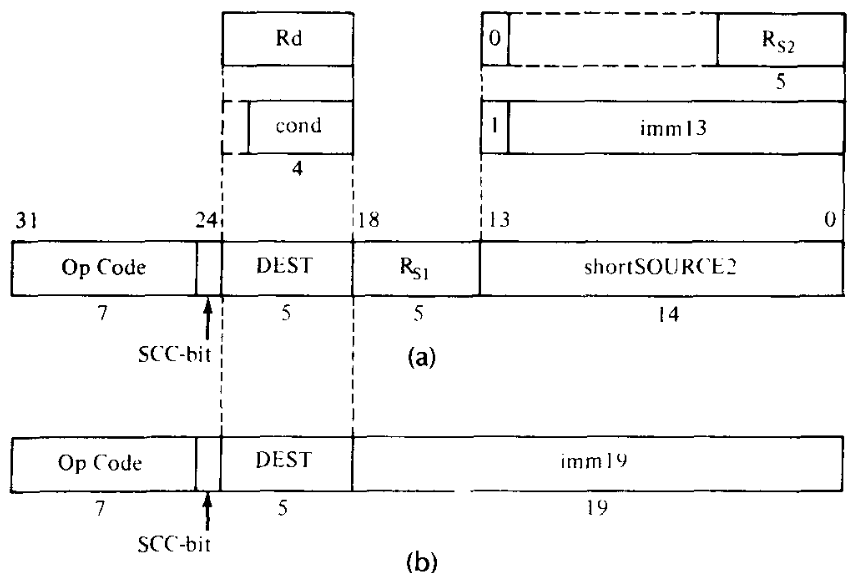
\includegraphics[width=0.75\linewidth]{Original/InstructionFormatStallings.png}
    \caption{Formato de instrução do RISC~I\cite{stallings_reduced_1988}.}
    \label{fig:instructionFormat}
\end{figure}

O formato com o imediato longo é utilizado em instruções relativas, onde o imediato longo é adicionado ao contador de programa para obter um endereço relativo ao atual. Ele também é utilizado na instrução \textit{Load High Immediate} (LDHI), onde os 19 bits são carregados para os bits mais significativos, permitindo o carregamento de constantes que ocupem os 32 bits dos registradores em menos ciclos do que com instruções de carregamento normais. Já o formato com imediato curto é utilizado para quaisquer outras instruções.

Para ambos os formatos, os 3 primeiros parâmetros são iguais. Os primeiros 7 bits representam a instrução que deve ser executada, seguidos de uma \textit{flag} (um bit) para definir códigos de condição, indicando se a instrução deve gravar as \textit{flags} de resultado da ULA na PSW. A última parte possui 5 bits, que podem representar um endereço de destino do resultado ou uma condição. Caso seja uma condição, apenas os 4 bits menos significativos são usados, com o quinto sendo ignorado.

Para o formato com imediato curto, os primeiros 5 bits após o destino são sempre um registrador fonte. Este registrador fonte é então seguido de uma segunda fonte, que pode ser tanto um registrador quanto um imediato de 13 bits. Para que o imediato seja escolhido, o primeiro bit após a primeira fonte deverá ser 1, seguido do valor desejado para o imediato. Caso o bit após a primeira fonte seja 0, os 5 bits menos significativos representam o registrador que será utilizado como segunda fonte.

\subsection{Conjunto de Instruções}

\begin{table}[!htp]\centering
\scriptsize
\begin{tabular}{ccccccccccc}\toprule
\cellcolor[HTML]{b7b7b7} &\cellcolor[HTML]{b7b7b7}- &0 &1 &2 &3 &4 &5 &6 &7 \\
\cellcolor[HTML]{b7b7b7}+ &\cellcolor[HTML]{b7b7b7} &----000 &\cellcolor[HTML]{d9ead3}----001 &----010 &\cellcolor[HTML]{d9ead3}----011 &----100 &\cellcolor[HTML]{d9ead3}----101 &----110 &\cellcolor[HTML]{d9ead3}----111 \\\midrule
0 &0000--- &\cellcolor[HTML]{b4a7d6}CALLI &\cellcolor[HTML]{9fc5e8}SLL &\cellcolor[HTML]{cc0000} &\cellcolor[HTML]{ead1dc}STS &\cellcolor[HTML]{c9daf8}AND &\cellcolor[HTML]{d0e0e3}SUB &\cellcolor[HTML]{351c75}\textcolor{white}{RET} &\cellcolor[HTML]{a61c00}\textcolor{white}{LDHI} \\
1 &\cellcolor[HTML]{d9ead3}0001--- &\cellcolor[HTML]{b4a7d6} &\cellcolor[HTML]{9fc5e8} &\cellcolor[HTML]{cc0000} &\cellcolor[HTML]{d5a6bd}STRS &\cellcolor[HTML]{c9daf8} &\cellcolor[HTML]{d0e0e3} &\cellcolor[HTML]{351c75} &\cellcolor[HTML]{a61c00} \\
2 &0010--- &\cellcolor[HTML]{b4a7d6} &\cellcolor[HTML]{93c47d}GETPSW &\cellcolor[HTML]{cc0000} &\cellcolor[HTML]{ead1dc} &\cellcolor[HTML]{c9daf8} &\cellcolor[HTML]{a2c4c9}SUBC &\cellcolor[HTML]{351c75} &\cellcolor[HTML]{a61c00} \\
3 &\cellcolor[HTML]{d9ead3}0011--- &\cellcolor[HTML]{b4a7d6} &\cellcolor[HTML]{93c47d} &\cellcolor[HTML]{cc0000} &\cellcolor[HTML]{d5a6bd} &\cellcolor[HTML]{c9daf8} &\cellcolor[HTML]{a2c4c9} &\cellcolor[HTML]{351c75} &\cellcolor[HTML]{a61c00} \\
4 &0100--- &\cellcolor[HTML]{b4a7d6} &\cellcolor[HTML]{9fc5e8} &\cellcolor[HTML]{fce5cd}LDBU &\cellcolor[HTML]{c27ba0}STB &\cellcolor[HTML]{a4c2f4}XOR &\cellcolor[HTML]{76a5af}SUBR &\cellcolor[HTML]{20124d}\textcolor{white}{RETI} &\cellcolor[HTML]{a61c00} \\
5 &\cellcolor[HTML]{d9ead3}0101--- &\cellcolor[HTML]{b4a7d6} &\cellcolor[HTML]{9fc5e8} &\cellcolor[HTML]{f9cb9c}LDRBU &\cellcolor[HTML]{a64d79}STRB &\cellcolor[HTML]{a4c2f4} &\cellcolor[HTML]{76a5af} &\cellcolor[HTML]{20124d} &\cellcolor[HTML]{a61c00} \\
6 &0110--- &\cellcolor[HTML]{b4a7d6} &\cellcolor[HTML]{93c47d} &\cellcolor[HTML]{f6b26b}LDBS &\cellcolor[HTML]{c27ba0} &\cellcolor[HTML]{a4c2f4} &\cellcolor[HTML]{45818e}SUBCR &\cellcolor[HTML]{20124d} &\cellcolor[HTML]{a61c00} \\
7 &\cellcolor[HTML]{d9ead3}0111--- &\cellcolor[HTML]{b4a7d6} &\cellcolor[HTML]{93c47d} &\cellcolor[HTML]{e69138}LDRBS &\cellcolor[HTML]{a64d79} &\cellcolor[HTML]{a4c2f4} &\cellcolor[HTML]{45818e} &\cellcolor[HTML]{20124d} &\cellcolor[HTML]{a61c00} \\
8 &1000--- &\cellcolor[HTML]{8e7cc3}CALL &\cellcolor[HTML]{6fa8dc}SRL &\cellcolor[HTML]{b45f06}\textcolor{white}{LDW} &\cellcolor[HTML]{741b47}\textcolor{white}{STW} &\cellcolor[HTML]{6d9eeb}OR &\cellcolor[HTML]{134f5c}\textcolor{white}{ADD} &\cellcolor[HTML]{cc4125}\textcolor{white}{GETLPC} &\cellcolor[HTML]{a61c00} \\
9 &\cellcolor[HTML]{d9ead3}1001--- &\cellcolor[HTML]{8e7cc3} &\cellcolor[HTML]{6fa8dc} &\cellcolor[HTML]{fff2cc}LDRW &\cellcolor[HTML]{4c1130}\textcolor{white}{STRW} &\cellcolor[HTML]{6d9eeb} &\cellcolor[HTML]{134f5c} &\cellcolor[HTML]{cc4125} &\cellcolor[HTML]{a61c00} \\
A &1010--- &\cellcolor[HTML]{e6b8af}JMP &\cellcolor[HTML]{6aa84f}PUTPSW &\cellcolor[HTML]{b45f06} &\cellcolor[HTML]{741b47} &\cellcolor[HTML]{6d9eeb} &\cellcolor[HTML]{134f5c} &\cellcolor[HTML]{cc4125} &\cellcolor[HTML]{a61c00} \\
B &\cellcolor[HTML]{d9ead3}1011--- &\cellcolor[HTML]{e6b8af} &\cellcolor[HTML]{6aa84f} &\cellcolor[HTML]{fff2cc} &\cellcolor[HTML]{4c1130} &\cellcolor[HTML]{6d9eeb} &\cellcolor[HTML]{134f5c} &\cellcolor[HTML]{cc4125} &\cellcolor[HTML]{a61c00} \\
C &1100--- &\cellcolor[HTML]{674ea7}\textcolor{white}{CALLR} &\cellcolor[HTML]{3d85c6}SRA &\cellcolor[HTML]{ffe599}LDSU &\cellcolor[HTML]{741b47} &\cellcolor[HTML]{6d9eeb} &\cellcolor[HTML]{0c343d}\textcolor{white}{ADDC} &\cellcolor[HTML]{cc4125} &\cellcolor[HTML]{a61c00} \\
D &\cellcolor[HTML]{d9ead3}1101--- &\cellcolor[HTML]{674ea7} &\cellcolor[HTML]{3d85c6} &\cellcolor[HTML]{ffd966}LDRSU &\cellcolor[HTML]{4c1130} &\cellcolor[HTML]{6d9eeb} &\cellcolor[HTML]{0c343d} &\cellcolor[HTML]{cc4125} &\cellcolor[HTML]{a61c00} \\
E &1110--- &\cellcolor[HTML]{dd7e6b}JMPR &\cellcolor[HTML]{3d85c6} &\cellcolor[HTML]{f1c232}LDSS &\cellcolor[HTML]{741b47} &\cellcolor[HTML]{6d9eeb} &\cellcolor[HTML]{0c343d} &\cellcolor[HTML]{cc4125} &\cellcolor[HTML]{a61c00} \\
F &\cellcolor[HTML]{d9ead3}1111--- &\cellcolor[HTML]{dd7e6b} &\cellcolor[HTML]{3d85c6} &\cellcolor[HTML]{bf9000}\textcolor{white}{LDRSS} &\cellcolor[HTML]{4c1130} &\cellcolor[HTML]{6d9eeb} &\cellcolor[HTML]{0c343d} &\cellcolor[HTML]{cc4125} &\cellcolor[HTML]{a61c00} \\
\bottomrule
\end{tabular}
\caption{Conjunto de instruções do RISC~I(adaptação de \citeonline{peek_vlsi_1983})}\label{tab:instructionSet}
\end{table}

A tabela \ref{tab:instructionSet} mostra todas as instruções existentes no RISC~I. Algumas das instruções tiveram os seus nomes modificados para melhorar a consistência e legibilidade, mas todas mantém as suas funções originais. Das alterações que foram feitas temos a remoção do caractere "X" em instruções como "JMPX", "LDXW", "STXW" ou "CALLX", pois este "X" representa que a instrução utiliza um registrador ao invés de um operante relativo, o que se torna desnecessário já que as instruções que usam relativo já são marcadas com um "R", além de que o "X" pode ser confuso para entender apenas de olhar a instrução. As instruções de subtração foram alteradas para não usar a letra "I", no lugar elas usam "R", um padrão usado por \citeonline{stallings_reduced_1988} que ajuda a não confundir com outras instruções que envolvem interrupções e que também terminam em "I". "GTLPC" foi alterado para "GETLPC" para ficar consistente com a instrução "GETPSW". Por fim, para instruções de \textit{Load} e \textit{Store} foram adotadas as letras "B" para as que utilizam apenas \textit{bytes}, e "S" para as que utilizam \textit{shorts}(\textit{2 bytes}).

\begin{table}[!htp]\centering
\fontsize{6.5pt}{10.25pt}\selectfont
\begin{tabular}{lrccrrrr}\toprule
\cellcolor[HTML]{A8A8A8}Mnemonico &\cellcolor[HTML]{A8A8A8}Nome completo &\cellcolor[HTML]{A8A8A8}HEX &\cellcolor[HTML]{A8A8A8}BIN &\multicolumn{3}{c}{\cellcolor[HTML]{A8A8A8}Operação} \\\midrule
CALLI &\textbf{CALL} WITH \textbf{I}NTERRUPT &00 &000 0XXX &CWP-- &\multicolumn{2}{c}{Rd <= Last pc} \\
CALL &\textbf{CALL} &08 &000 100X &CWP-- &Rd <= pc &Next pc <= Rx + S2 \\
JMP &CONDITIONAL \textbf{J}U\textbf{MP} &0A &000 101X &\multicolumn{3}{c}{pc <= Rx+S2} \\
CALLR &\textbf{CALL} \textbf{R}ELATIVE &0C &000 110X &CWP-- &Rd <= pc &Next pc <= pc + Y \\
JMPR &CONDITIONAL \textbf{J}U\textbf{MP} \textbf{R}ELATIVE &0E &000 111X &\multicolumn{3}{c}{pc <= pc + Y} \\
SLL &\textbf{S}HIFT \textbf{L}EFT \textbf{L}OGICAL &10 &001 0X0X &\multicolumn{3}{c}{Rd <= Rs << S2} \\
GETPSW &\textbf{GET} \textbf{P}ROCESSOR \textbf{S}TATUS \textbf{W}ORD &12 &001 0X1X &\multicolumn{3}{c}{Rd <= PSW} \\
SRL &\textbf{S}HIFT \textbf{R}IGHT \textbf{L}OGICAL &18 &001 100X &\multicolumn{3}{c}{Rd <= Rs >> S2} \\
PUTPSW &\textbf{PUT} \textbf{P}ROCESSOR \textbf{S}TATUS \textbf{W}ORD &1A &001 101X &\multicolumn{3}{c}{PSW <= Rm} \\
SRA &\textbf{S}HIFT \textbf{R}IGHT \textbf{A}RITHMETIC &1C &001 11XX &\multicolumn{3}{c}{Rd <= Rs >>> S2} \\
LDBU &\textbf{L}OA\textbf{D} \textbf{B}YTE \textbf{U}NSIGNED &24 &010 0100 &\multicolumn{3}{c}{Rd <= M[Rx+S2]} \\
LDRBU &\textbf{L}OA\textbf{D} \textbf{R}ELATIVE \textbf{B}YTE \textbf{U}NSIGNED &25 &010 0101 &\multicolumn{3}{c}{Rd <= M[pc+Y]} \\
LDBS &\textbf{L}OA\textbf{D} \textbf{B}YTE \textbf{S}IGNED &26 &010 0110 &\multicolumn{3}{c}{Rd <= M[Rx+S2]} \\
LDRBS &\textbf{L}OA\textbf{D} \textbf{R}ELATIVE \textbf{B}YTE \textbf{S}IGNED &27 &010 0111 &\multicolumn{3}{c}{Rd <= M[pc+Y]} \\
LDW &\textbf{L}OA\textbf{D} \textbf{W}ORD &28 &010 10X0 &\multicolumn{3}{c}{Rd <= M[Rx+S2]} \\
LDRW &\textbf{L}OA\textbf{D} \textbf{R}ELATIVE \textbf{W}ORD &29 &010 10X1 &\multicolumn{3}{c}{Rd <= M[pc+Y]} \\
LDSU &\textbf{L}OA\textbf{D} \textbf{S}HORT \textbf{U}NSIGNED &2C &010 1100 &\multicolumn{3}{c}{Rd <= M[Rx+S2]} \\
LDRSU &\textbf{L}OA\textbf{D} \textbf{R}ELATIVE \textbf{S}HORT \textbf{U}NSIGNED &2D &010 1101 &\multicolumn{3}{c}{Rd <= M[pc+Y]} \\
LDSS &\textbf{L}OA\textbf{D} \textbf{S}HORT \textbf{S}IG\textbf{}NED &2E &010 1110 &\multicolumn{3}{c}{Rd <= M[Rx+S2]} \\
LDRSS &\textbf{L}OA\textbf{D} \textbf{R}ELATIVE \textbf{S}HORT \textbf{S}IGNED &2F &010 1111 &\multicolumn{3}{c}{Rd <= M[pc+Y]} \\
STS &\textbf{ST}ORE \textbf{S}HORT &30 &011 00X0 &\multicolumn{3}{c}{M[Rx+S2] <= Rm} \\
STRS &\textbf{ST}ORE \textbf{R}ELATIVE \textbf{S}HORT &31 &011 00X1 &\multicolumn{3}{c}{M[pc+Y] <= Rm} \\
STB &\textbf{ST}ORE \textbf{B}YTE &34 &011 01X0 &\multicolumn{3}{c}{M[Rx+S2] <= Rm} \\
STRB &\textbf{ST}ORE \textbf{R}ELATIVE \textbf{B}YTE &35 &011 01X1 &\multicolumn{3}{c}{M[pc+Y] <= Rm} \\
STW &\textbf{ST}ORE \textbf{W}ORD &38 &011 1XX0 &\multicolumn{3}{c}{M[Rx+S2] <= Rm} \\
STRW &\textbf{ST}ORE \textbf{R}ELATIVE \textbf{W}ORD &39 &011 1XX1 &\multicolumn{3}{c}{M[pc+Y] <= Rm} \\
AND &\textbf{AND} &40 &100 00XX &\multicolumn{3}{c}{Rd <= Rs \& S2} \\
XOR &E\textbf{X}CLUSIVE \textbf{OR} &44 &100 01XX &\multicolumn{3}{c}{Rd <= Rs \^ S2} \\
OR &\textbf{OR} &48 &100 1XXX &\multicolumn{3}{c}{Rd <= Rs | S2} \\
SUB &\textbf{SUB}TRACT &50 &101 000X &\multicolumn{3}{c}{Rd <= Rs - S2} \\
SUBC &\textbf{SUB}TRACT WITH \textbf{C}ARRY &52 &101 001X &\multicolumn{3}{c}{Rd <= Rs - S2 - C} \\
SUBR &\textbf{SUB}TRACT \textbf{R}EVERSED &54 &101 010X &\multicolumn{3}{c}{Rd <= S2 - Rs} \\
SUBCR &\textbf{SUB}TRACT WITH \textbf{C}ARRY \textbf{R}EVERSED &56 &101 011X &\multicolumn{3}{c}{Rd <= S2 - Rs - C} \\
ADD &\textbf{ADD} &58 &101 10XX &\multicolumn{3}{c}{Rd <= Rs + S2} \\
ADDC &\textbf{ADD} WITH \textbf{C}ARRY &5C &101 11XX &\multicolumn{3}{c}{Rd <= Rs + S2 + C} \\
RET &\textbf{RET}URN &60 &110 00XX &pc <=Rx+S2 &\multicolumn{2}{c}{Next CWP++} \\
RETI &\textbf{RET}URN WITH \textbf{I}NTERRUPT &64 &110 01XX &pc <=Rx+S2 &\multicolumn{2}{c}{Next CWP++} \\
GETLPC &\textbf{GET L}AST \textbf{P}ROGRAM \textbf{C}OUNTER &68 &110 1XXX &\multicolumn{3}{c}{Rd <= Last pc} \\
LDHI &\textbf{L}OA\textbf{D} \textbf{H}IGH \textbf{I}MMEDIATE &70 &111 XXXX &\multicolumn{3}{c}{Rd <= (Y[31:13],13'0)} \\
\bottomrule
\end{tabular}
\caption{Instruções do RISC~I}\label{tab:instructionSetDetail }
\end{table}

\subsection{\textit{Datapath}}\label{cap:datapath}
\begin{figure}[H]
    \centering
    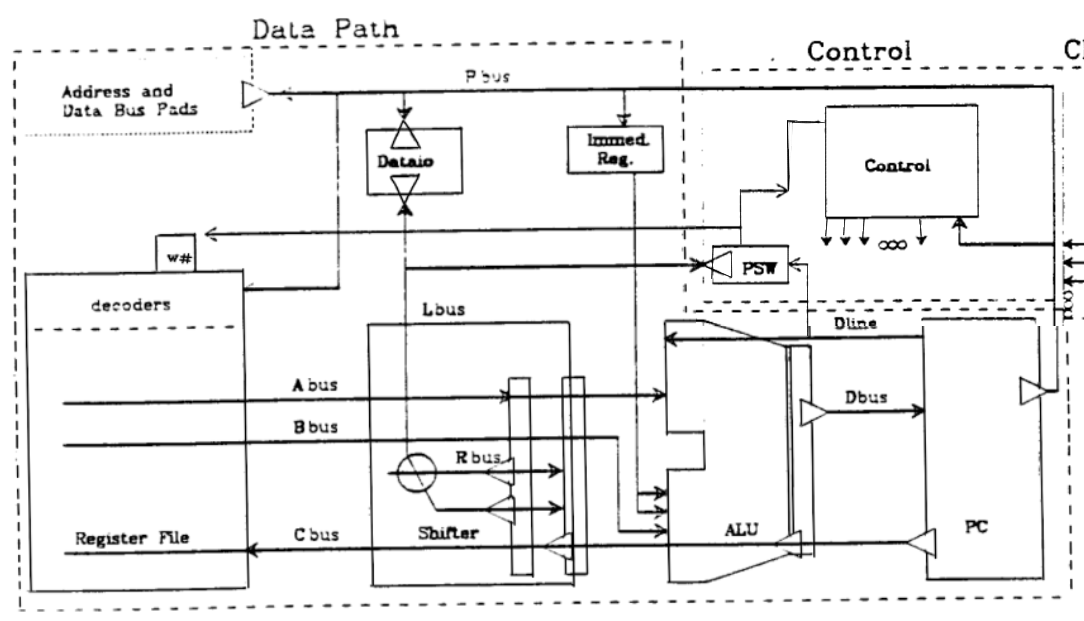
\includegraphics[width=0.75\linewidth]{Original/datapathPeek.png}
    \caption{\textit{Datapath} do RISC I\cite{peek_vlsi_1983}}
    \label{fig:riscDatapathPeek}
\end{figure}
A figura \ref{fig:riscDatapathPeek} mostra uma visão um pouco mais detalhada do RISC em comparação a outros trabalhos relacionados. Ela mostra componentes que geralmente são omitidos como o \textit{DataIO}, que serve como \textit{buffer} de entrada e saída de informações, o registrador imediato, o número de janela e o registrador de estado do processador(PSW). 
uma boa parte dos barramentos é mostrado de forma atravessada sobre certos componentes pois é assim que estes são colocados no chip como descrito por Peek. Nesse trabalho, como tentativa de deixar as informações mais visíveis, os barramentos não passam por cima dos componentes, no caso os barramentos A, B e C passam abaixo de alguns dos componentes enquanto a linha D passa por cima, como demonstrado na figura \ref{fig:riscDatapath}. 

Vale notar que o trabalho disponível do Peek possui erros de impressão nos seus diagramas, onde linhas verticais ficam falhadas. Para tentar diminuir erros, foi executada uma restauração nos diagramas, porém alguns ainda podem conter falta de informações. A conexão entre o PSW, o número da janela estava apagada no trabalho original o que dificulta o entendimento das conexões. Isso veio junto com uma inconsistência, onde há um diagrama que demonstra que o controlador do número de janela se conecta a PSW através do barramento L. A solução para a implementação no simulador foi utilizar a conexão pelo barramento D como demonstrado na figura \ref{fig:riscDatapath}.

\begin{figure}[H]
    \centering
    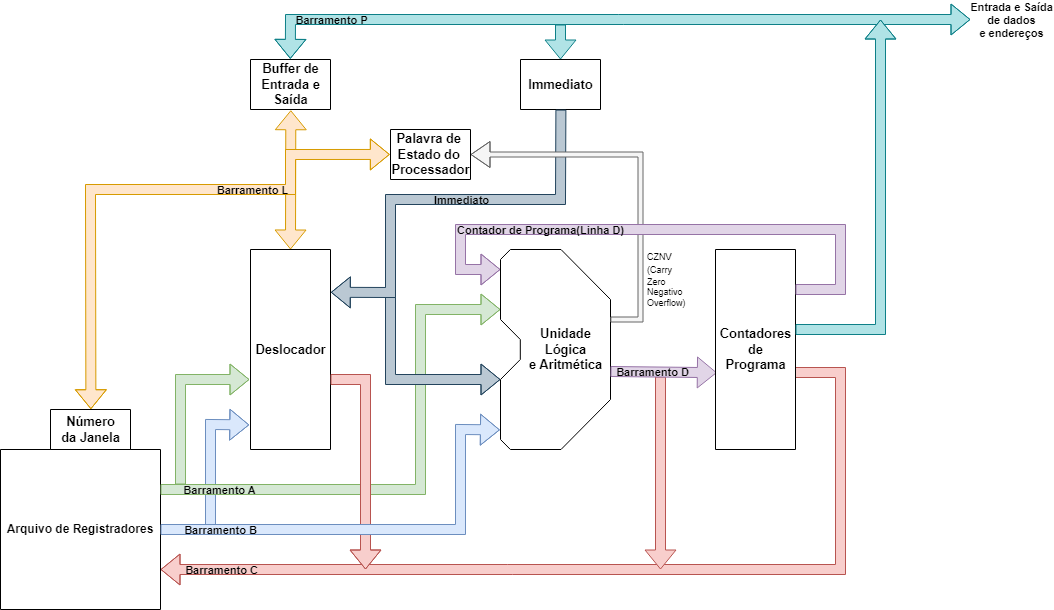
\includegraphics[width=0.75\linewidth]{ArquiteturaRISCI.png}
    \caption{Arquitetura do RISC I(autoria própria).(Note que componentes de controle e \textit{clock} foram omitidos)}
    \label{fig:riscDatapath}
\end{figure}

Uma alteração foi realizada entre a unidade lógica e aritmética(ULA) e o contador de programa(PC). No trabalho original, o resultado da ULA se separa internamente entre duas saídas, uma para o barramento C, e outro negada para o barramento D. A negação para o barramento D se deve a implementação física, onde os barramentos A, B, C e D são pré-carregados em alta voltagem, e são lidos descarregando as conexões onde há zeros, resultando em uma inversão da informação. A saída para o barramento C não precisa ser invertida, porque ela é armazenada em registradores que são lidos apenas através dos barramentos A ou B, que invertem a informação de volta ao que era originalmente. O barramento D por outro lado, se conecta diretamente ao contador de programa, que precisa que a informação não esteja negada, pois essa informação são os endereços que são passados para o barramento P, que não é pré-carregado.

Como a implementação no simulador não necessita de pré carregamento dos barramentos, a ULA nesta implementação possui apenas uma saída que conecta ao barramento D. O barramento D ainda conecta a ULA ao PC, porém foi adicionado uma conexão controlada(através de \textit{buffers tri-state}) ao barramento C. Em uma visão geral, esta mudança não altera o funcionamento dos recursos da arquitetura sendo equivalente ao que foi implementado originalmente.

\subsection{Temporização}\label{cap:timing}
A temporização do RISC~I funciona a partir de 3 fases por instrução, o que geralmente envolve o carregamento de alguma informação durante a fase 1, uma execução durante a fase 2 e finalmente o armazenamento do resultado durante a fase 3. 

As instruções de \textit{store} e \textit{load} possuem um ciclo secundário (denominado com um \textbf{s}), que ocorre entre as fases 2 e 3 do ciclo normal de instruções(denominado com um \textbf{n}). Este ciclo secundário ocorre pois para a execução dessas instruções primeiro é necessário calcular o endereço de memória que será utilizado para depois este ser enviado a memória para que a informação seja retornada, o que exige o ciclo adicional. 

Além do ciclo secundário para instruções de \textit{load} e \textit{store} existe o ciclo de interrupção. Este ciclo ocorre quando algum problema ou erro ocorre durante a instrução atual. No RISC~I isso envolve o \textit{overflow} ou \textit{underflow} do número de janela de registradores. Para que a interrupção ocorra, também é necessário que a \textit{flag} de interrupções esteja ativa(será discutido na seção \ref{cap:clock}). A interrupção é detectada durante o fase 1, e caso ocorra, as fases 2i e 3i são executadas, forçando a próxima instrução a ser um "CALLI" e enviando o vetor de de interrupção para a memória, que seria o endereço que possui a rotina de tratamento da interrupção.
\begin{figure}
    \centering
    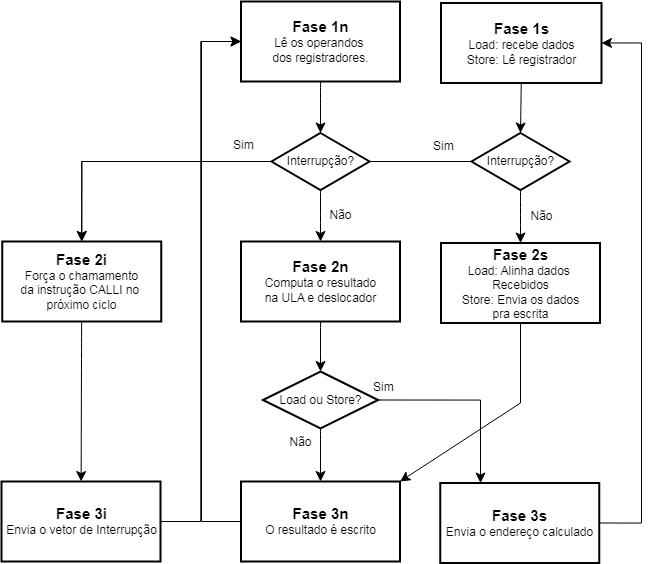
\includegraphics[width=0.75\linewidth]{Logisim/temporizaçãorisc.png}
    \caption{Temporização do RISC I (adaptado de \citeonline{peek_vlsi_1983}}
    \label{fig:temporizationDiagram}
\end{figure}

\subsection{\textit{Pipeline}}
A \textit{pipeline} de instruções é uma técnica que melhora o desempenho do processador ao dividir a execução de uma instrução em várias etapas, como busca, decodificação, cálculo de operandos, busca de operandos e execução. Semelhante a uma linha de montagem, onde diferentes estágios de produção ocorrem simultaneamente, a \textit{pipeline} permite que várias instruções sejam processadas ao mesmo tempo em diferentes estágios. No entanto, a eficiência da \textit{pipeline} pode ser afetada por fatores como o tempo de execução ser maior que o tempo de busca e instruções de desvio condicional que tornam o endereço da próxima instrução desconhecido. Para mitigar esses problemas, técnicas como a predição de desvios são utilizadas, permitindo um aumento significativo na velocidade de execução das instruções. \cite[p.~47-51]{stallings_reduced_1988}

\begin{figure}
    \centering
    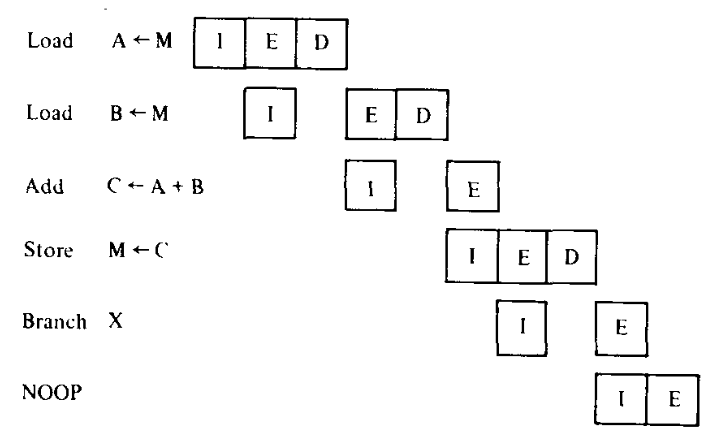
\includegraphics[width=0.5\linewidth]{pipelineRISCI.png}
    \caption{Demonstração da \textit{pipeline} do RISC~I.\cite{stallings_reduced_1988}}
    \label{fig:pipelineRISCI}
\end{figure}
A \textit{pipeline} do RISC~I(Figura \ref{fig:pipelineRISCI}) é bem simples, ela se divide em duas etapas: A busca da próxima instrução seguida da execução.  O fato da pipeline ser tão simples pode ajudar a simplificar o entendimento de como uma \textit{pipeline} funciona. Na busca da próxima instrução é possível ver que o processador esta acessando um certo endereço que esta sendo lido e separado entre varias partes pelo circuito. Enquanto isso, é possível também ver os barramentos A,B e C trocando dados como instruído no endereço que estava sendo lido anteriormente. Além disso, diversos registradores mostram no simulador qual é a próxima coisa que será utilizada e qual esta sendo utilizada no momento.

\section{Implementação}
\subsection{Limitações da simulação e principais diferenças da implementação física}\label{cap:limitations}
Os simuladores de circuitos lógicos são ferramentas poderosas para o desenvolvimento e teste de sistemas digitais. No entanto, esses simuladores possuem limitações que devem ser consideradas. Primeiramente, os simuladores de circuitos lógicos, como o Logisim, são incapazes de replicar com precisão todos os aspectos físicos dos circuitos reais, como atrasos de propagação e efeitos parasitas. Além disso, certos comportamentos complexos e interações entre componentes podem não ser completamente modelados, resultando em discrepâncias entre a simulação e o desempenho real do circuito.

Para poder executar essa implementação, algumas medidas foram tomadas para que o modelo funcione corretamente. Uma destas medidas já foi citada na seção \ref{cap:datapath}, onde foi removida a negação do barramento D pelo diferente funcionamento dentro do simulador, onde os barramentos não precisam ser pré carregados. 

Outra modificação que foi realizada foi a alteração de todos os \textit{latches} para \textit{flip flops}. Na implementação original, \textit{latches} foram utilizados em diversos dos componentes, porém certos problemas de sincronização surgiram durante a replicação do circuito e foi decidido a substituição para \textit{flip flops}. Com essa modificação ao invés dos registradores armazenarem os valores durante o nível alto, eles apenas gravam durante a subida(ou descida)de \textit{clock}, ajudando na sincronia entre componentes e evitando erros.

Como será discutido no capítulo \ref{cap:controller}, o circuito de controle foi uma das maiores diferenças sobre o circuito original. Isso se deve tanto a falta de informações nos documentos originais quanto a diferenças de implementação nos componentes. Apesar disso o resultado final da execução do conjunto de instruções é igual em ambas implementações.

Uma limitação menos significativa do Logisim é a falta de suporte para conectores que são simultaneamente de entrada e saída(conhecidas como \textit{inout}). Este tipo de conexão tem uma certa importância para poder conectar barramentos a certas partes do circuito, porém pode ser simulada utilizando uma entrada e uma saída, uma a frente da outra no pacote de componente como mostrado no capítulo \ref{cap:dataio}.

\subsection{Componentes e Simbologia do Logisim Evolution}

O Logisim Evolution oferece componentes prontos para uso em circuitos lógicos. Eles podem servir desde funções lógicas básicas até operações mais complexas, como armazenamento de dados ou decodificação.
\begin{figure}[H]
    \centering
    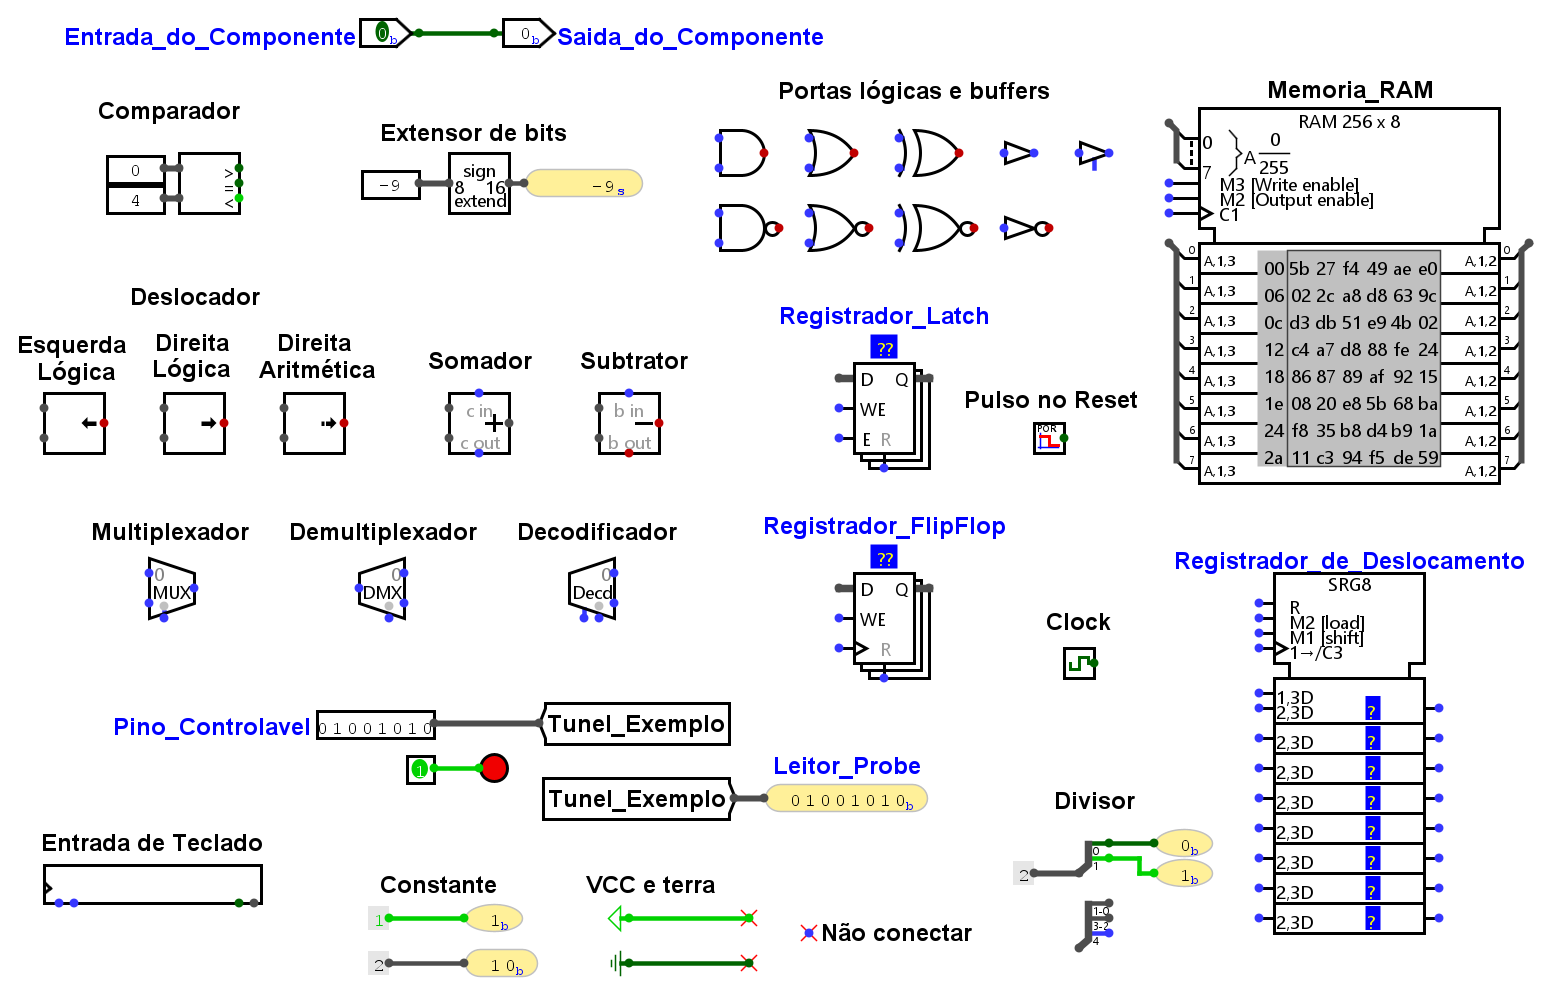
\includegraphics[width=0.75\linewidth]{Logisim/LogisimSimbologia.png}
    \caption{Componentes do Logisim utilizados no trabalho}
    \label{fig:logisimComponents}
\end{figure}

A Figura \ref{fig:logisimComponents} mostra todos os componentes nativos utilizados para a criação do modelo de simulação. Muitos desses componentes podem ter suas propriedades modificadas, o que também pode alterar sua aparência, quantidade de saídas e entradas. No simulador, todas as operações lógicas são suportadas, além de \textit{buffers} que apenas permitem a passagem de informações de um lado para outro, e \textit{buffers tri-state}, que permitem a passagem de dados apenas quando ativos, ficando em alta impedância caso contrário.

Operações de deslocamento podem ser realizadas pelo mesmo componente, desde que suas propriedades sejam modificadas. Operações aritméticas também são suportadas; entretanto, neste trabalho, foi utilizado apenas o subtrator e o somador. O simulador também oferece multiplexadores e de-multiplexadores, que permitem a seleção de uma entre várias conexões para a entrada ou saída de dados. Há também o decodificador, que permite a decodificação de um número binário para um número decimal.

Além das operações comuns, o simulador suporta componentes que armazenam um certo valor até que a simulação reinicie, como os pinos, ou componentes que permanecem com o mesmo valor, como as constantes. Para conectar dois fios sem que eles estejam visivelmente conectados no simulador, podemos usar túneis; todos os túneis com o mesmo nome se comportam como se estivessem conectados ao mesmo fio. Para ler os valores, utilizamos um leitor, ou \textit{probe}, que mostra qual é o valor do fio ou barramento ao qual está conectado. Esse valor pode ser verificado posteriormente em um histórico de valores.

Todas as conexões podem ter quatro estados diferentes, que são diferenciados pelas cores: verde claro (1), verde escuro (0), azul (?,Z ou alta impedância), e vermelho (X ou erro/curto). Todas essas cores podem ser identificadas em fios que possuem apenas 1 bit de dado sendo transmitido; no entanto, há a possibilidade de criar barramentos que utilizam múltiplos bits. No tema original, a cor para esses barramentos é branca, mas neste trabalho foi alterada para cinza devido à troca da cor de fundo. O simulador possui componentes que podem dividir ou combinar de diversas formas um barramento entre vários outros.

Também é possível criar nossos próprios componentes, que podem ter sua aparência modificada. Neste trabalho, a aparência será referenciada como "pacote". O pacote pode conter entradas e saídas, que são definidas quando componentes específicos de entrada e saída são colocados dentro do circuito do componente. O pacote dos componentes pode conter caixas de texto que indicam o valor dos registradores dentro desses componentes.

\subsection{Circuito de \textit{clock}}\label{cap:clock}
\begin{figure}[H]
    \centering
    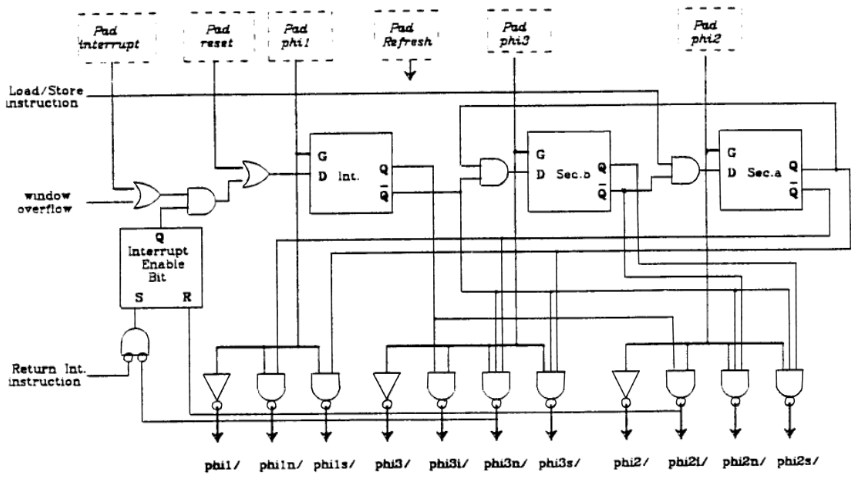
\includegraphics[width=0.75\linewidth]{Original/clockPeek.png}
    \caption{Circuito de \textit{clock} do RISC~I \cite{peek_vlsi_1983}}
    \label{fig:clockPeek}    
\end{figure}
O circuito de \textit{clock} do RISC~I é responsável por controlar o funcionamento dos ciclos e fases da arquitetura descritos na seção \ref{cap:timing}. Ele possui uma entrada para cada fase e diversas saídas contendo a fase junto com o tipo de ciclo, este sendo normal(n), secundário(s) e de interrupção(i). 

Para o controle de qual tipo de ciclo esta sendo executado, este circuito possui \textit{flip flops} para armazenar se uma interrupção esta ocorrendo e se uma instrução de save/load esta ocorrendo. Para a interrupção ocorrer, há um \textit{flip flop} que deve estar ativo, o \textit{Interrupt\_Enable}, que é ligado durante a instrução "RETI".

Na implementação realizada no Logisim, as saídas das fases não foram invertidas, e o mesmo ocorre na entrada das portas logicas conectadas ao \textit{Interrupt\_Enable}. Funcionalmente isso não fez diferença para a arquitetura, e os possíveis efeitos disso foram tratados no controlador e outros componentes que fazem uso direto dos sinais de fase.
\begin{figure}[H]
    \centering
    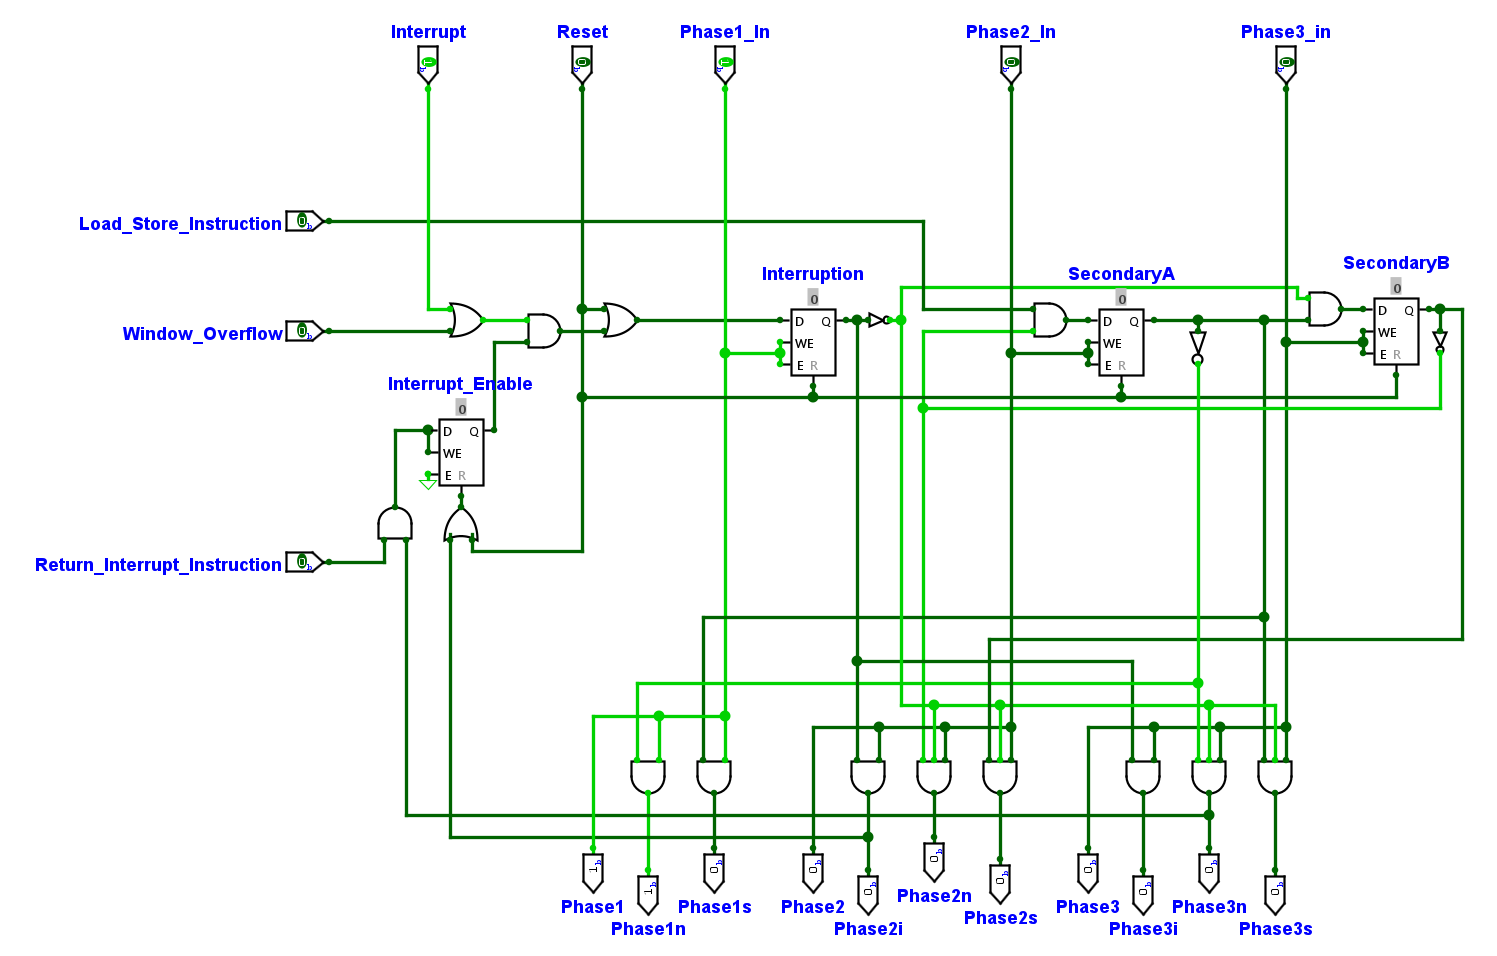
\includegraphics[width=0.75\linewidth]{Logisim/clock.png}
    \caption{Circuito de \textit{clock} no Logisim}
    \label{fig:clock}
\end{figure}
O pacote do componente visto na figura \ref{fig:clockPack} mostra as entradas de fases por cima e as saídas à direita. À esquerda foram colocados os sinais de controle. Foram adicionados textos para cada um dos \textit{flip flops}, ao lado da entrada ou saída que os representam.

\begin{figure}[H]
        \centering
        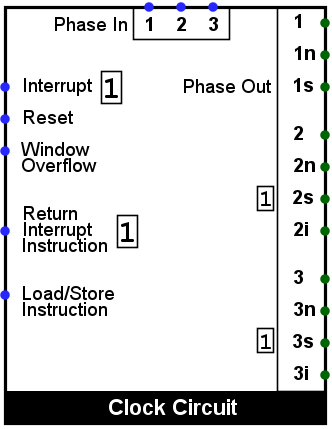
\includegraphics[width=0.25\linewidth]{Logisim/clockPack.png}
        \caption{Pacote do circuito de \textit{clock} no Logisim}
        \label{fig:clockPack}
    \end{figure}
    A entrada das fases do circuito de \textit{clock} são geradas por um circuito a parte, fora do chip principal. Este gerador foi implementado com 3 flip flops D em cadeia que quando recebem o sinal de \textit{reset} ficam com um ativo, que vai pro próximo em toda borda de descida do \textit{clock}.
\begin{figure}[H]
    \centering
    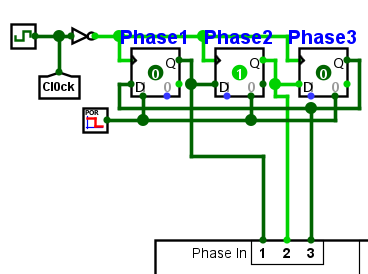
\includegraphics[width=0.25\linewidth]{Logisim/clockGenerator.png}
    \caption{Gerador de \textit{clock} e fases no Logisim}
    \label{fig:clockGen}
\end{figure}
\subsection{Contador de Programa}
\begin{figure}[H]
    \centering
    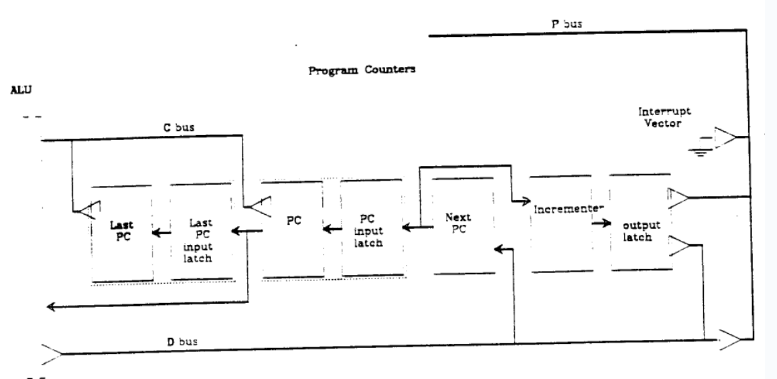
\includegraphics[width=0.75\linewidth]{Original/pcPeek.png}
    \caption{Contadores de programa\cite{peek_vlsi_1983}}
    \label{fig:pcPeek}
\end{figure}
O RISC~I possui um contador de programa dividido em 3 partes: O próximo, o atual e o anterior. No circuito original foram usados \textit{latches} \textit{master-slave}(ou \textit{flip flops}) tanto para o contador atual quanto para o anterior. O circuito original também faz uso de um \textit{latch} para a saída do próximo contador de programa, que é usado no primeiro ciclo da \textit{pipeline} para dizer qual é o próximo endereço a ser lido.

Para a implementação no Logisim, algumas modificações foram feitas. Os \textit{flip flops} foram colocados diretamente para cada um dos contadores no lugar de\textit{ latches master-slave}. O \textit{latch} de saída foi removido, o que causaria oscilação no próximo contador, porém com a troca de \textit{latch} para \textit{flip flop}, este problema foi resolvido.

Outro modificação que foi feita sobre o contador de programa foi a temporização dos sinais do controle. No trabalho de Peek é dito que: 
\begin{citacao}
O último \textit{latch} PC é carregado de seu \textit{latch} de entrada a cada Phi1n. Durante cada Phi2n, o próximo PC é passado para o \textit{latch} de entrada PC. O próximo PC é carregado do barramento D durante cada Phi3n e Phi3i. Os dados no barramento D vêm do incrementador para o fluxo normal de instruções; e da ALU para saltos. O incrementador opera de Phi3 para Phi1 e é válido por Phi2.
\end{citacao}
Porém ao seguir essa temporização, houveram problemas nas instruções "CALLI" e "GetLPC", além de que a atualização dessincronizada entre os contadores não faz sentido considerando seu contexto. Para corrigir isso, os 3 contadores se atualizam durante as 3n e 3i. Com essa alteração, também foi necessário trocar a saída do PC atual para o próximo PC, caso contrário, ao retornar de chamadas de "CALLI", o processador voltaria para a instrução de "CALL" ao invés da instrução seguinte.

Parte do controle de \textit{byte} foi transferido para dentro do contador de programa. Este é o registrador \textit{Byte\_Offset\_Reg}, que possui os 2 bits menos significativos de um endereço para instruções de \textit{store}. Estes 2 bits dizem em qual byte do endereço a informação esta ou será armazenada, por exemplo, se estes bits forem 10, a informação estará armazenada a partir do terceiro byte.

O vetor de interrupção foi modificado para retornar o número hexadecimal 80000000. Essa modificação se deve parcialmente a forma com que este vetor funciona no RISC~II, onde os endereços para tratamento de interrupções estão em torno deste valor\cite[p.~198]{katevenis_reduced_1985}. Outro motivo é que ao reiniciar a simulação, o contador de programa utiliza o endereço 0, o que causaria problemas caso este estivesse ocupado com uma rotina de tratamento de interrupção. Esse vetor, diferentemente da implementação original, é passado para o próximo PC, fazendo com que a próxima instrução a ser decodificada e executada seja a da interrupção.

\begin{figure}[H]
    \centering
    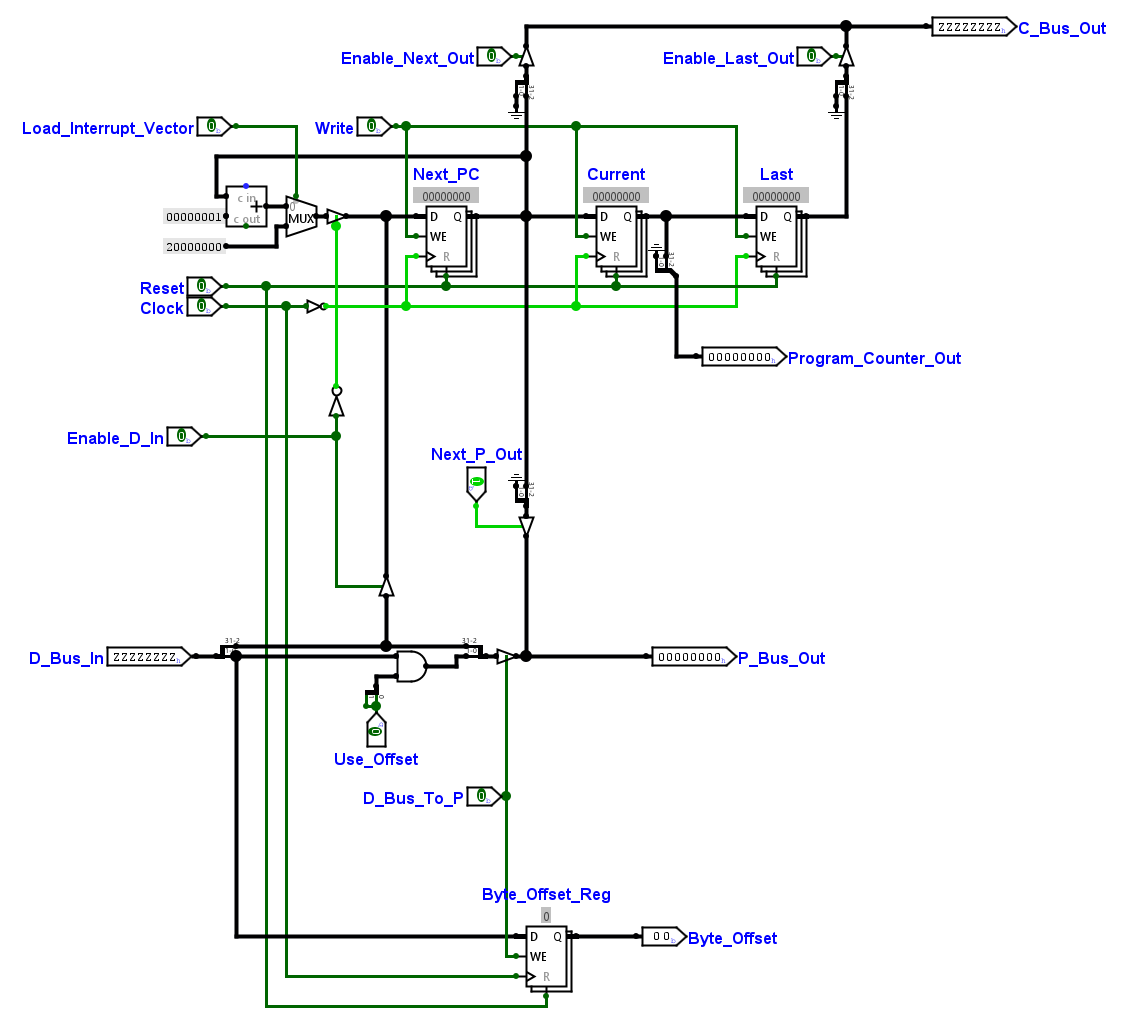
\includegraphics[width=0.75\linewidth]{Logisim/pc.png}
    \caption{Contadores de programa no Logisim}
    \label{fig:pc}
\end{figure}
O componente mostra o valor de cada um dos contadores em tamanho grande, um seguido pra outro, com a conexão indicado por uma seta. O número de seleção do \textit{byte} também foi adicionado ao lado de sua saída. Todas as entradas ficam à esquerda enquanto as saídas ficam à direita. em cima foram adicionados os sinais de \textit{clock} e \textit{reset}
\begin{figure}[H]
    \centering
    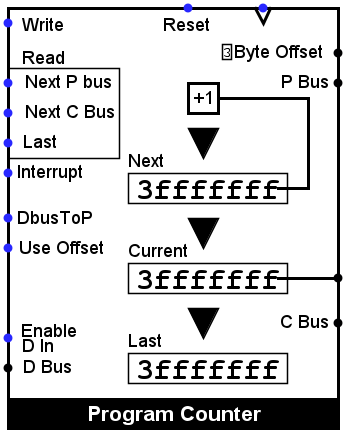
\includegraphics[width=0.25\linewidth]{Logisim/pcPack.png}
    \caption{Pacote dos contadores de programa no Logisim}
    \label{fig:pcPack}
\end{figure}
\subsection{Registrador Imediato}
\begin{figure}[H]
    \centering
    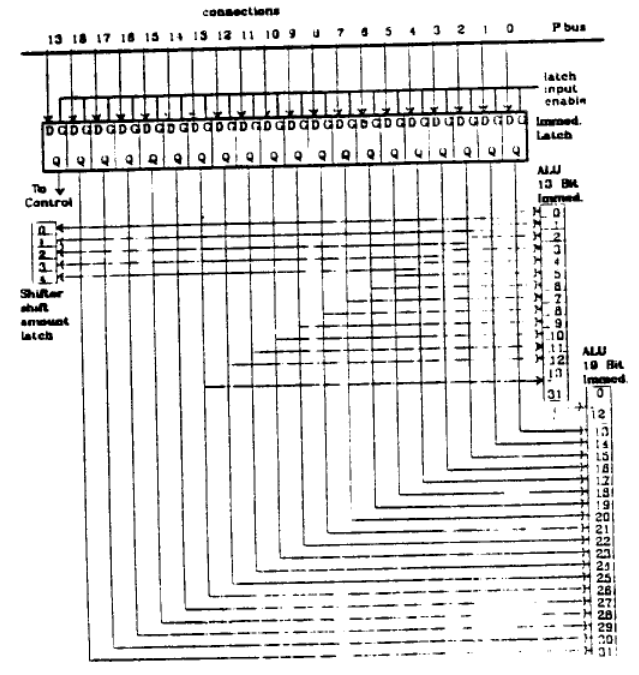
\includegraphics[width=0.75\linewidth]{Original/immediatePeek.png}
    \caption{Registrador imediato\cite{peek_vlsi_1983}}
    \label{fig:immediatePeek}    
\end{figure}
Para a implementação do imediato foi utilizado um \textit{flip flop} de 19 bits, similar a proposta do original. O diagrama original deixa a ideia de que a saída de 19 bits serve apenas para carregar os 19 bits mais significantes para a ula, porém como indicado por \citeonline[p.~40]{katevenis_reduced_1985}, as instruções relativas utilizam os 19 bits e não necessariamente carregados nos bits mais significantes. Para a seleção do\textit{ Load High} foi adicionada uma entrada no circuito como mostrado na figura \ref{fig:immediate}.

Katevenis também diz que a saída de 13 bits possui sinal estendido, que foi implementado no Logisim com um componente de extensor de bits, que também foi utilizado para estender os bits da saída de 19 bits. 

\begin{figure}[H]
    \centering
    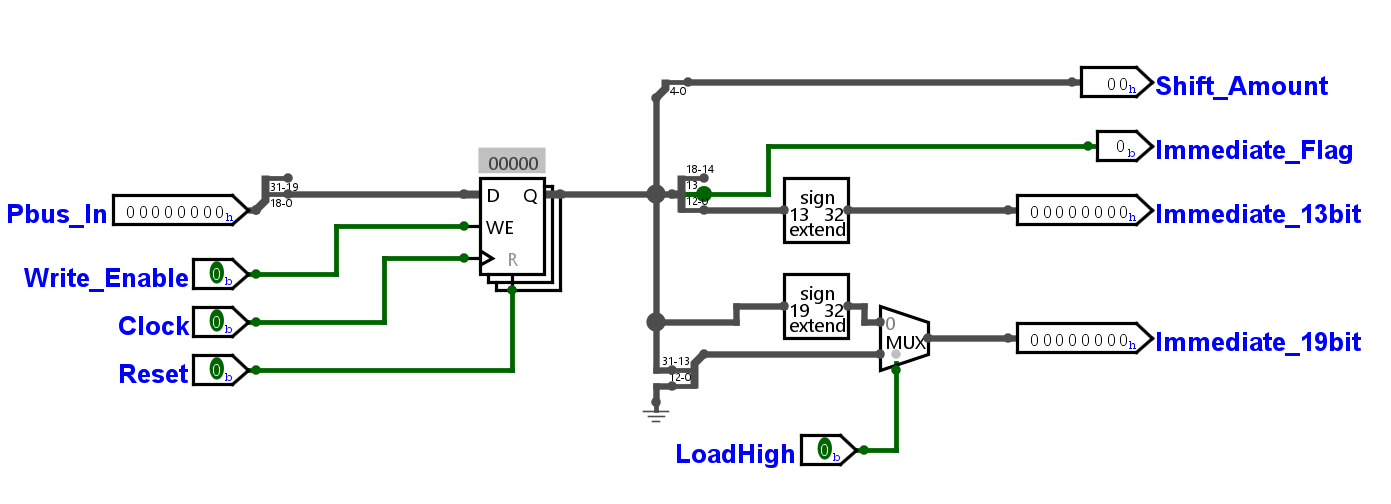
\includegraphics[width=0.75\linewidth]{Logisim/immediate.png}
    \caption{Registrador imediato no Logisim}
    \label{fig:immediate}
\end{figure}
O imediato possui todas suas saídas à direita e sinais de controle acima e à esquerda. Adicionalmente foi adicionado um texto com o valor atual do registrador. 
\begin{figure}[H]
    \centering
    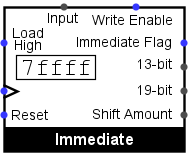
\includegraphics[width=0.25\linewidth]{Logisim/immediatePack.png}
    \caption{Pacote do registrador imediato no Logisim}
    \label{fig:immediatePack}
\end{figure}
\subsection{\textit{Buffer} de entrada e saída}\label{cap:dataio}
\begin{figure}[H]
    \centering
    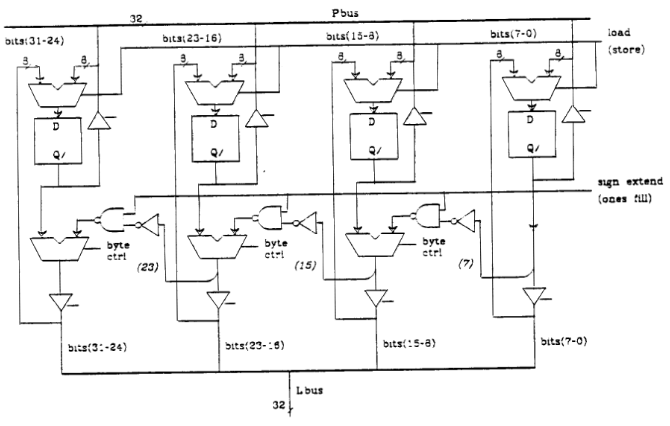
\includegraphics[width=0.75\linewidth]{Original/dataIOPeek.png}
    \caption{\textit{Buffer} de entrada e saída\cite{peek_vlsi_1983}}
    \label{fig:dataIOPeek}
\end{figure}
Para poder haver a troca de informações entre o processador e dispositivos de entrada e saída precisamos de um componente que consiga tratar esta troca de informações. Este componente é o \textit{buffer} de entrada e saída(\textit{dataIO}), que é responsável por receber e enviar dados para a memória do sistema através do barramento P, e estender o sinal caso a informação recebida não ocupe os 32 bits. 

No outro lado do \textit{dataIO} temos o barramento L, que é uma conexão com o deslocador, que também é utilizado ao carregar dados da memória. O \textit{dataIO} consegue através de \textit{buffers tri-state} alterar qual barramento esta recebendo informações e qual esta enviando. 

Na implementação do Logisim(figura \ref{fig:dataio}), parte do controle de byte(um componente de controle separado na implementação original) foi adicionado ao circuito. Esta parte é o decodificador de byte, que recebe qual é o tamanho da informação(8, 16 e 32 bits) e qual é o seu deslocamento(8, 16 ou 24 bits), como por exemplo, um byte pode estar tanto nos 8 bits mais significativos quanto nos 8 menos significativos. A informação decodificada então controla os \textit{muxes} que selecionam quais \textit{bytes} vão receber a informação e quais serão estendidos. Dos que são estendidos, estes podem estendidos por sinal ou com zeros, o que é definido pela entrada de controle de dado com sinal(\textit{Signed\_Data})
\begin{figure}[H]
    \centering
    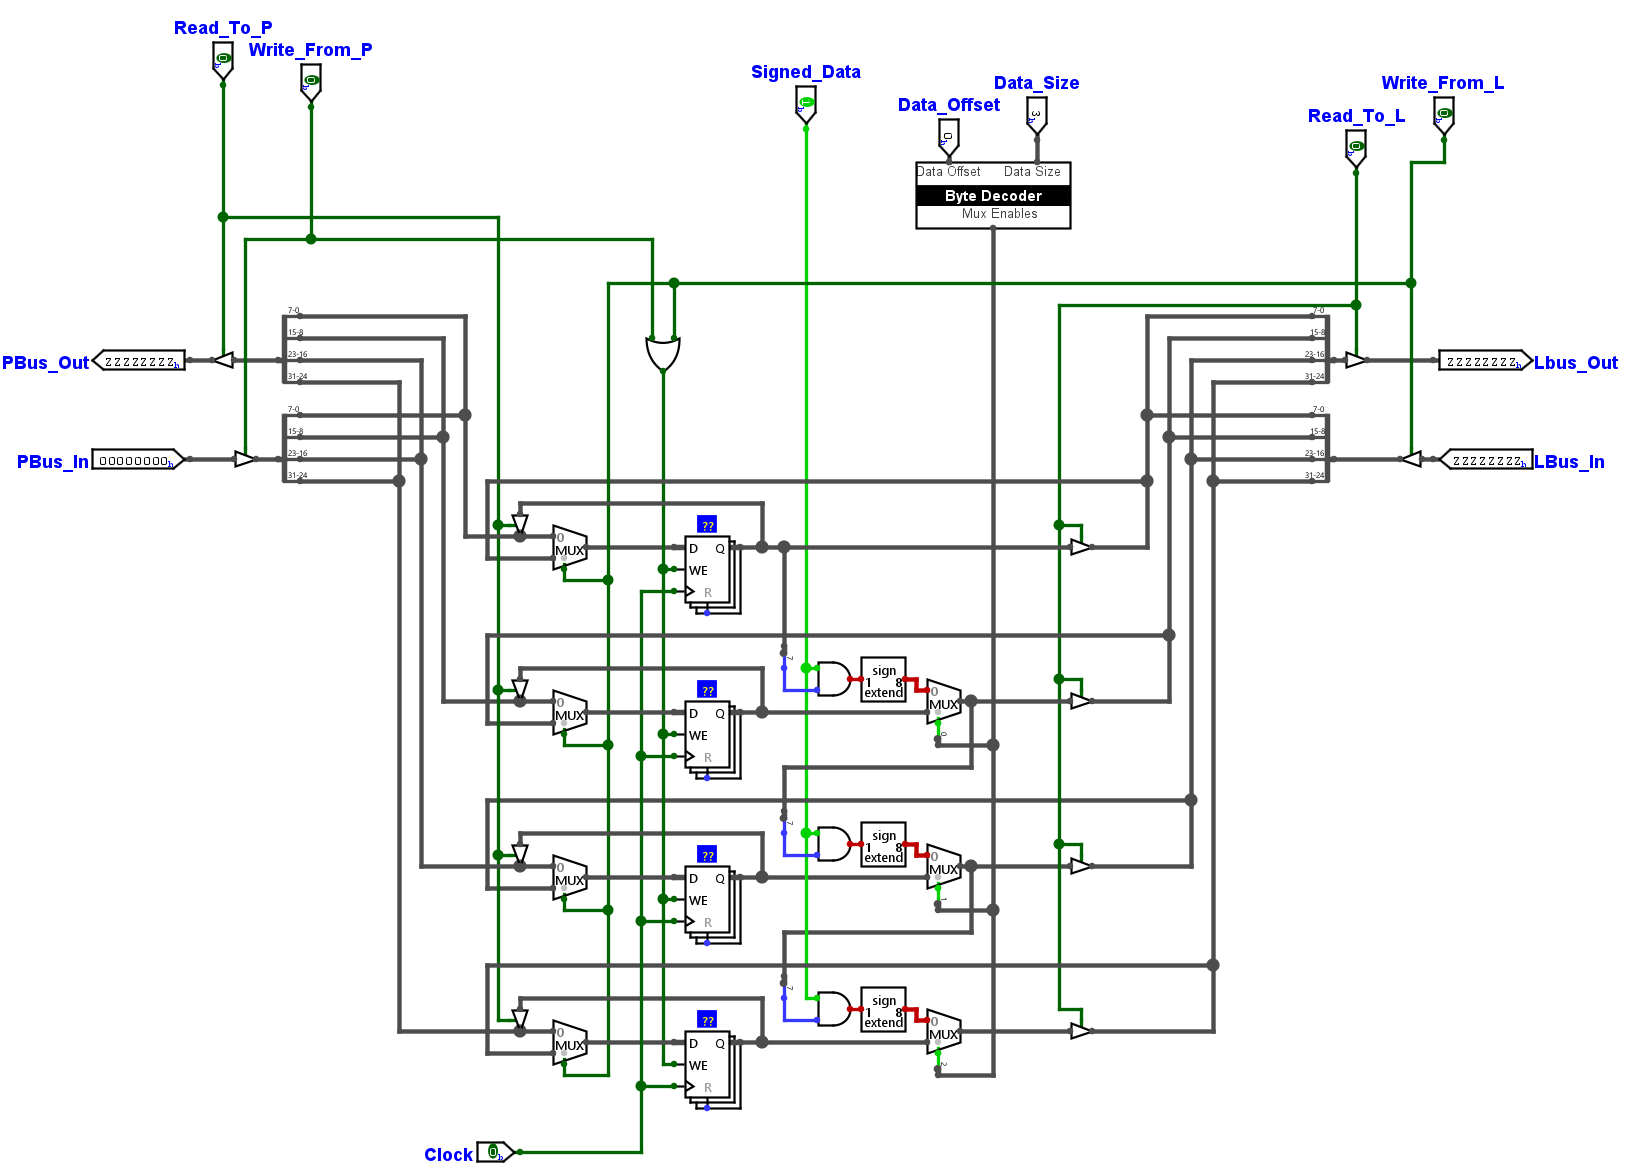
\includegraphics[width=0.75\linewidth]{Logisim/dataio.png}
    \caption{Circuito do \textit{buffer} de entrada e saída no Logisim}
    \label{fig:dataio}
\end{figure}
O componente do dataIO possui uma certa simetria, onde tanto em baixo quanto em cima há a entrada e saída dos barramento, um controle para leitura e outro para escrita. Como dito na seção \ref{cap:limitations}, as conexões que são tanto entrada quanto saída precisam ser recriadas usando uma entrada e uma saída. Como o Logisim não permite que a entrada e saída fiquem no mesmo lugar, uma das duas conexões é colocada à frente da outra, permitindo que um fio passe por elas e as conecte. Os sinais de controle de \textit{byte} ficaram à direita do componente enquanto o clock ficou à esquerda.
\begin{figure}[H]
    \centering
    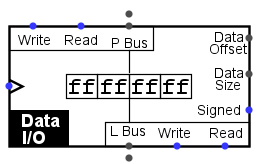
\includegraphics[width=0.25\linewidth]{Logisim/dataioPack.png}
    \caption{Pacote do \textit{buffer} de entrada e saída no Logisim}
    \label{fig:dataioPack}
\end{figure}

\subsection{Unidade Lógica e Aritmética}
\begin{figure}[H]
    \centering
    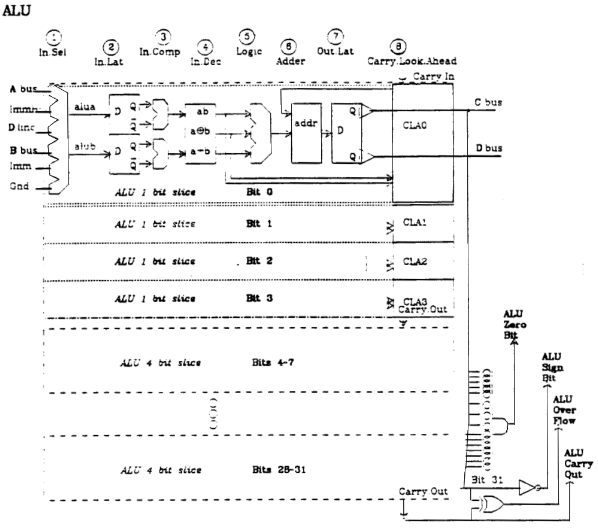
\includegraphics[width=0.75\linewidth]{Original/ALU.png}
    \caption{Unidade lógica e aritmética\cite{peek_vlsi_1983}}
    \label{fig:aluPeek}    
\end{figure}

A Implementação original da Unidade Lógica e Aritmética(ULA) possui 7 entradas de valores(Barramentos A e B, imediato de 13 e 19 bits, contador de programa, conexão terra e \textit{carry} in) e 6 saídas(barramentos C e D, e as \textit{flags} zero, sinal, \textit{overflow} e \textit{carry out}). Ela pode ser separada entre 8 partes, porém para a implementação no simulador, houve uma simplificação nos circuitos, resultando em 6 partes:
\begin{enumerate}
    \item Seleção de entrada: Na implementação do Logisim(figura \ref{fig:aluLogisim}), esta foi feita utilizando 2 \textit{muxes}, um para a entrada do primeiro parâmetro, que escolhe entre o barramento A, o Contador de Programa e a conexão terra, enquanto o outro seleciona entre os imediatos e o barramento B.
    \item \textit{Latch} de entrada: Dois \textit{latches}(\textit{flip flops} no Logisim) recebem as entradas que foram selecionadas no passo anterior durante a descida de \textit{clock} com o pino de escrita da ULA ligado, geralmente na fase 1.
    \item Troca de operantes: Na implementação original esta parte seria um complementador, porém o trabalho do Peek não explica direito como o complemento dos operadores é utilizado, sem contar que não há nenhuma operação puramente de complementação documentada. No Logisim, esta parte é utilizada para trocar os operantes A e B, para assim realizar as operações de subtração onde o B deve vir primeiro. Para alterar a ordem dos operantes, foi designado o bit 4 da entrada de operação como controle dos \textit{muxes}.
    \item Cálculo de operações: Os operantes então passam por diversos circuitos que calculam as operações da ULA. Diferentemente da implementação original, a implementação desse trabalho inclui um bloco de adição e subtração diretamente nessa seção para simplificar o circuito mantendo a mesma funcionalidade. Os circuitos aritméticos possuem saídas de \textit{carry out} que são selecionadas a partir de um \textit{mux} controlado pelo segundo bit da entrada da operação.      
    \item Seleção do resultado: O resultado é então escolhido por um \textit{mux} que recebe a entrada do operador como controle.
    \item \textit{Latch} de saída: Um \textit{latch}, que também foi implementado com um \textit{flip flop} no Logisim, salva o resultado da operação durante a fase 2 para poder ser finalmente lida na fase 3. As \textit{flags} de resultado, comumente chamadas de CNZV, representam respectivamente \textit{carry}, negativo, zero e \textit{overflow}, e são apenas válidas após a escrita do \textit{flip flop} de saída.
\end{enumerate}

\begin{figure}[H]
    \centering
    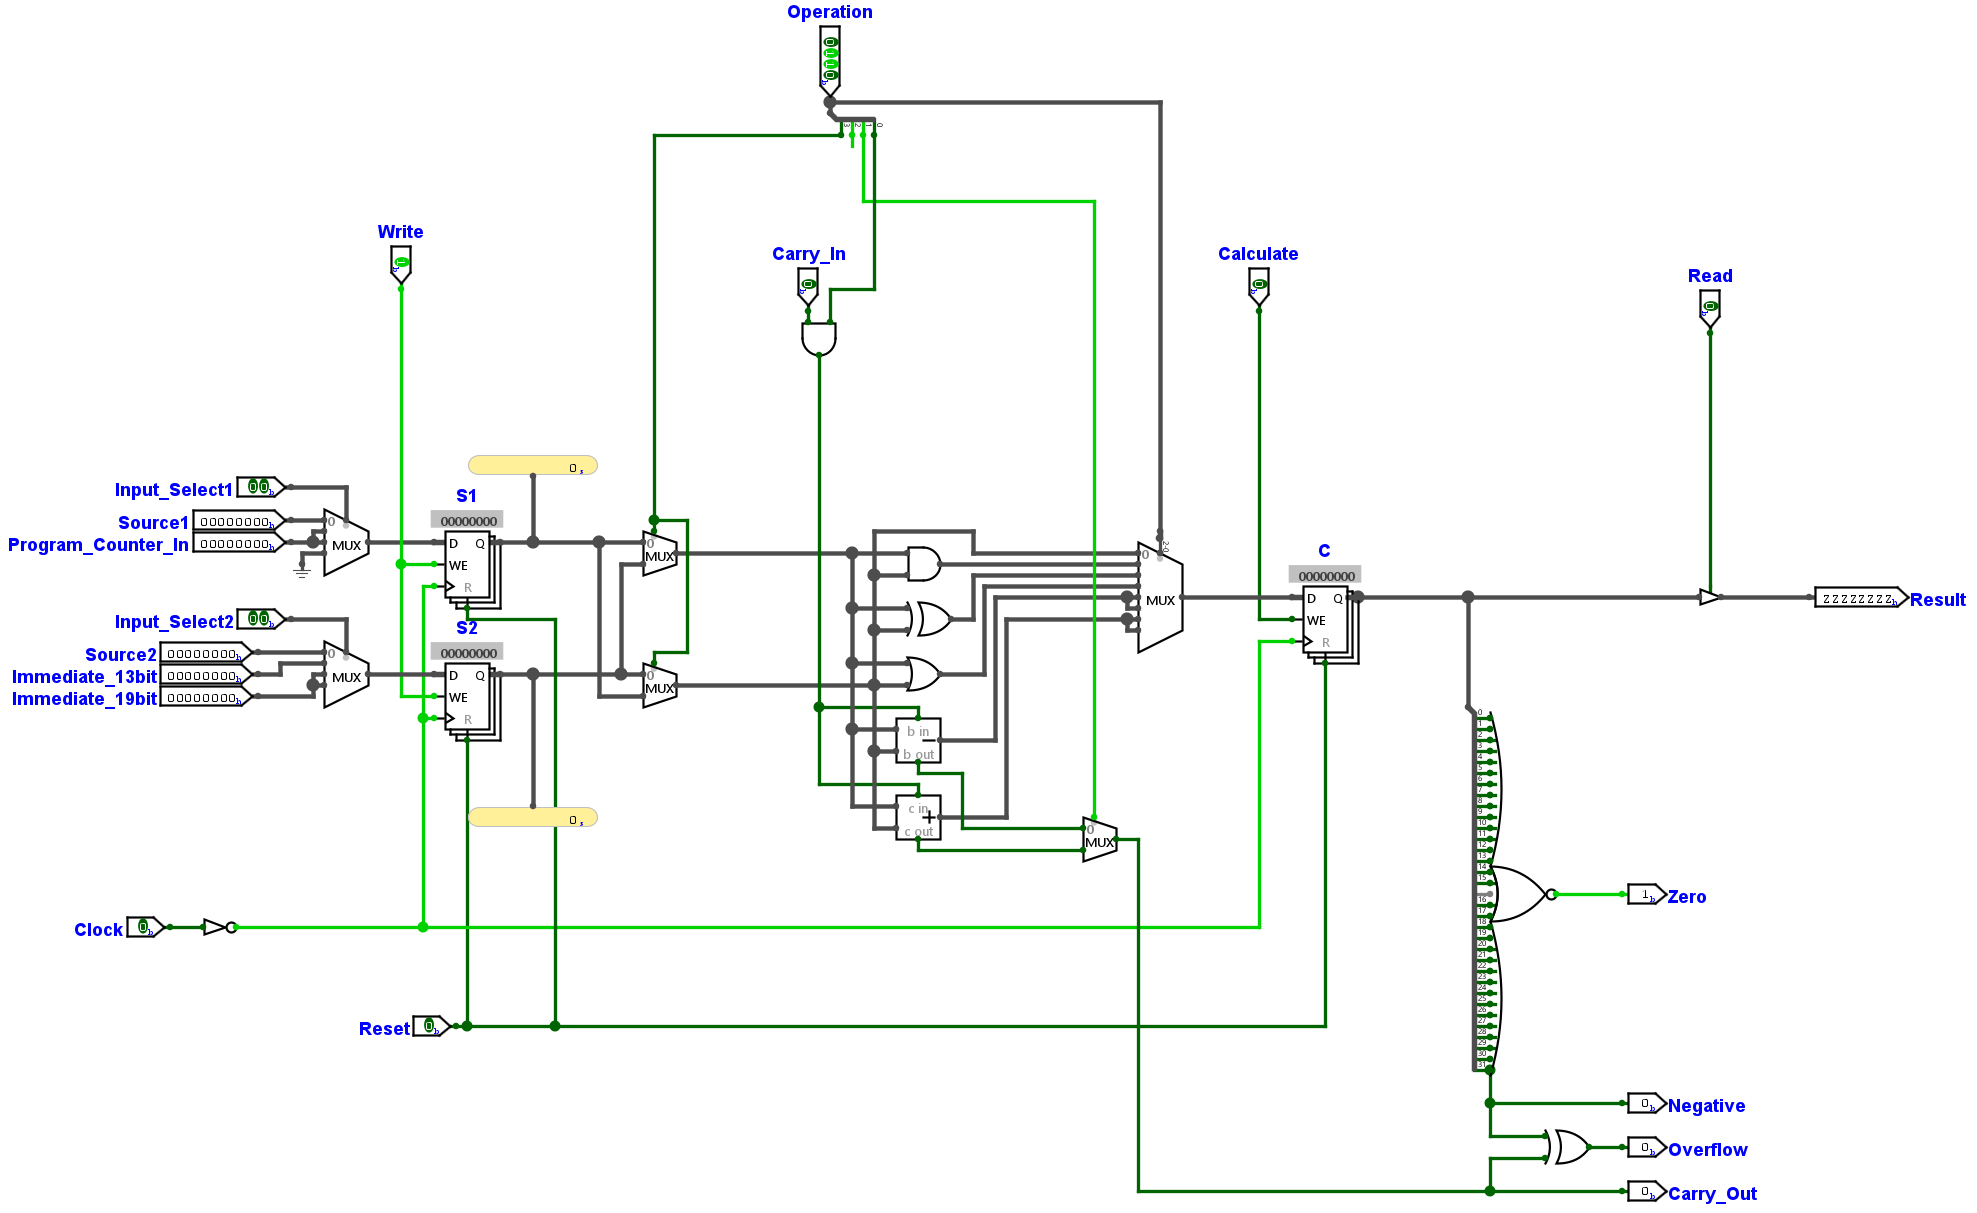
\includegraphics[width=0.75\linewidth]{Logisim/alu.png}
    \caption{Implementação da ULA no Logisim}
    \label{fig:aluLogisim}
\end{figure}
Para a representação visual do componente, adotou-se o formato comumente utilizado em diagramas de arquiteturas, conforme ilustrado na Figura \ref{fig:aluPack}. As entradas da Fonte 1, o seletor correspondente e o \textit{carry in} estão posicionados à esquerda, na parte superior da ULA. Na parte inferior esquerda, encontram-se a seleção da Fonte 2 e suas respectivas entradas. A seleção de operação, o \textit{clock} e o \textit{reset} estão centralizados no lado esquerdo. Os sinais de leitura, execução e escrita estão localizados acima do componente. Por fim, a saída das \textit{flags} e do resultado final está à direita do componente. 

\begin{figure}[H]
    \centering
    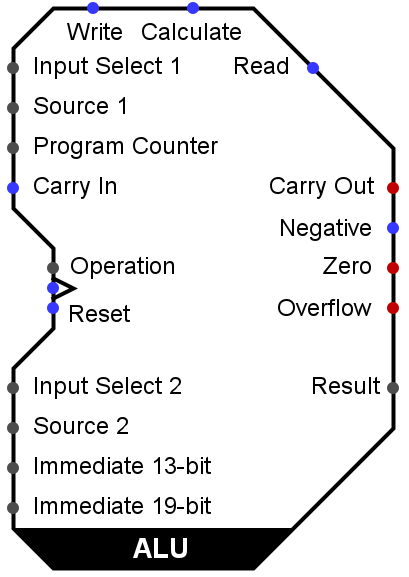
\includegraphics[width=0.25\linewidth]{Logisim/aluPack.png}
    \caption{Pacote da ULA no Logisim}
    \label{fig:aluPack}
\end{figure}
Apesar de ser considerado, não foi adicionado nenhum texto que mostre o valor dos registradores da ULA em seu pacote. isso se deve a falta de espaço utilizável, que torna difícil uma inserção desses textos sem aumentar o componente de tamanho. Futuramente isto pode ser reconsiderado, pois a exibição desses valores pode ser uma grande ajuda em passos de \textit{debugging}
\subsection{Deslocador}
\begin{figure}[H]
    \centering
    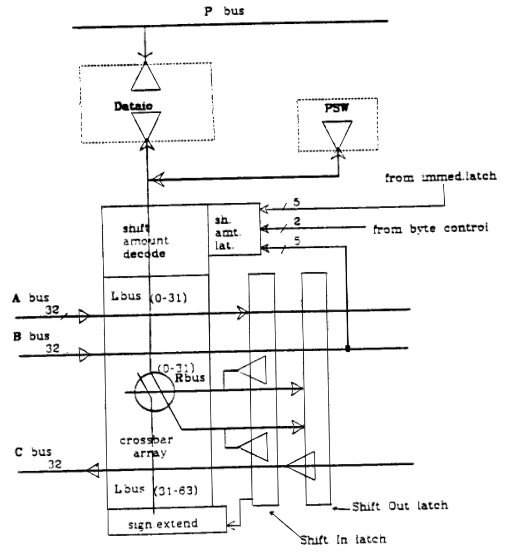
\includegraphics[width=0.75\linewidth]{Original/shifterPeek.png}
    \caption{Deslocador\cite{peek_vlsi_1983}}
    \label{fig:shifterPeek}
\end{figure}
O deslocador no RISC~I possui uma importância não só para a possibilidade de realizar cálculos de deslocamento, mas também porque ele serve como parte da interface para exterior do processador, juntamente com o \textit{dataIO}. Na implementação original ele possui dois barramentos internos, o barramento R(direita) e L(esquerda), que se conectam utilizando um matriz de conexões transversais, ou \textit{crossbar array}.

Ao invés de recriar o \textit{crossbar array}, foram utilizados diretamente os componentes de deslocamento de bits já prontos do \textit{Logisim}. Isso permite uma visualização mais simplificada do circuito final. O barramento R foi omitido enquanto o L foi mantido explicitamente para conexões externas como a do \textit{dataIO}.

Em instruções de carregamento, assim que uma informação é recebida, esta informação deve ser alinhada pelo deslocador caso ela não comece no primeiro byte. Para isso é realizado um deslocamento aritmético para a direita que alinha a informação ao primeiro byte, enquanto o sinal do valor é mantido.

Assim como a ULA, para haver sincronia de dados, os \textit{clocks} dos registradores de entrada foram invertidos, porém não houve necessidade dessa inversão no registrador de saída.
\begin{figure}[H]
    \centering
    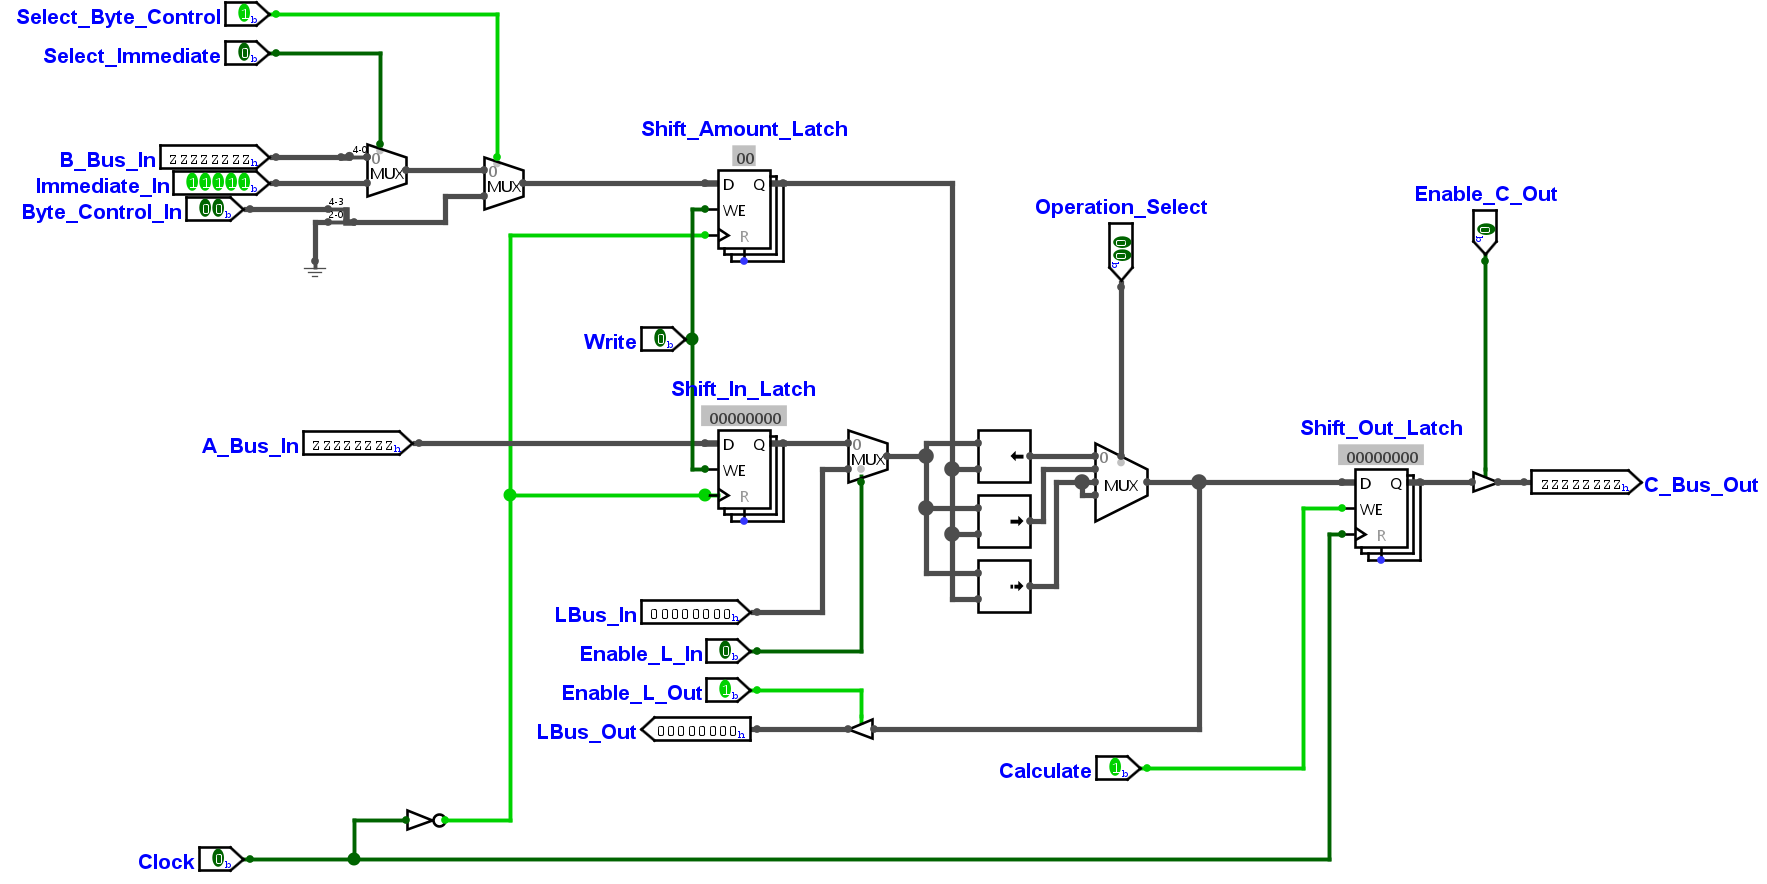
\includegraphics[width=0.75\linewidth]{Logisim/shifter.png}
    \caption{Deslocador no Logisim}
    \label{fig: shifter}
\end{figure}
Para o pacote do deslocador foram adicionados textos com os valores dos registradores de entrada e saída, além da quantidade de deslocamento. linhas foram adicionadas para indicar algumas das conexões internas de entrada e saída. À direita foram colocados sinais de controles gerais com a saída para o barramento C na parte mais inferior. À esquerda há a seleção da operação e da entrada da quantidade de deslocamento, com a entrada A na parte mais inferior. No Topo do deslocador ficam o \textit{clock} e a conexão de entrada e saída com o barramento L.
\begin{figure}[H]
    \centering
    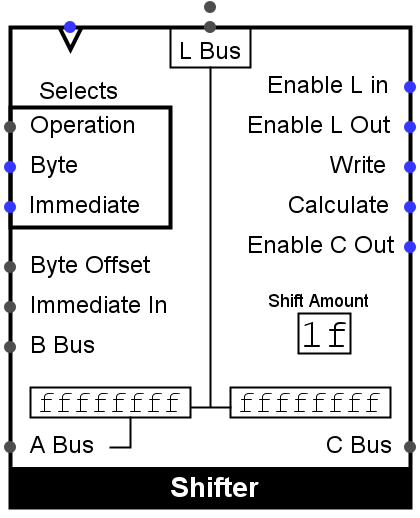
\includegraphics[width=0.25\linewidth]{Logisim/shifterPack.png}
    \caption{Pacote do deslocador no Logisim}
    \label{fig:shifterPack}
\end{figure}

\subsection{Arquivo de Registradores}\label{cap:registerFile}
\begin{figure}[H]
    \centering
    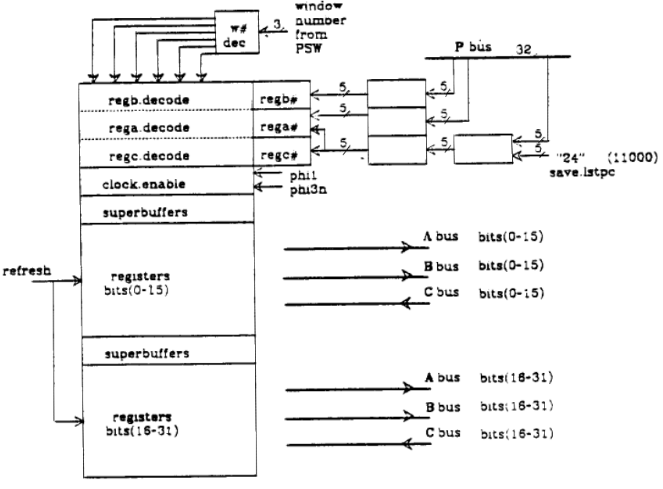
\includegraphics[width=0.75\linewidth]{Original/registerFilePeek.png}
    \caption{Arquivo de registradores\cite{peek_vlsi_1983}}
    \label{fig:registerFilePeek}
\end{figure}
O arquivo de registradores é uma das peças mais importantes da arquitetura RISC~I, permitindo a simplicidade de seu funcionamento. Nos chips RISC~I e RISC~II, ele ocupa a maior parte do chip e armazena informações de forma similar a uma pilha (\textit{stack}).

Os programas têm acesso a 32 registradores. O primeiro registrador é conectado ao terra, retornando 0 quando chamado e não sendo modificado quando utilizado como destino. 17 registradores são globais, e as últimas 14 conexões são dinâmicas, ligadas a diferentes grupos de registradores locais, chamados janelas. Essas janelas mudam a cada instrução de chamada e retorno, similar ao funcionamento de uma pilha. Os quatro primeiros registradores locais correspondem aos quatro últimos da janela anterior, permitindo o compartilhamento de parâmetros entre janelas.

O RISC~I original implementa apenas 6 janelas, mas com pequenas modificações no circuito, é possível adicionar mais 2, como no RISC~II. Na implementação realizada, foi utilizado o padrão de tamanho de janelas do RISC~II, com apenas nove registradores globais, mas 16 locais, dos quais seis são compartilhados entre janelas. Isso permite que mais parâmetros sejam passados pelos registradores em chamadas de funções e retornos, reduzindo a necessidade de armazenamento em memória com instruções de \textit{load} e \textit{store}, acelerando o processamento.
\begin{figure}[H]
    \centering
    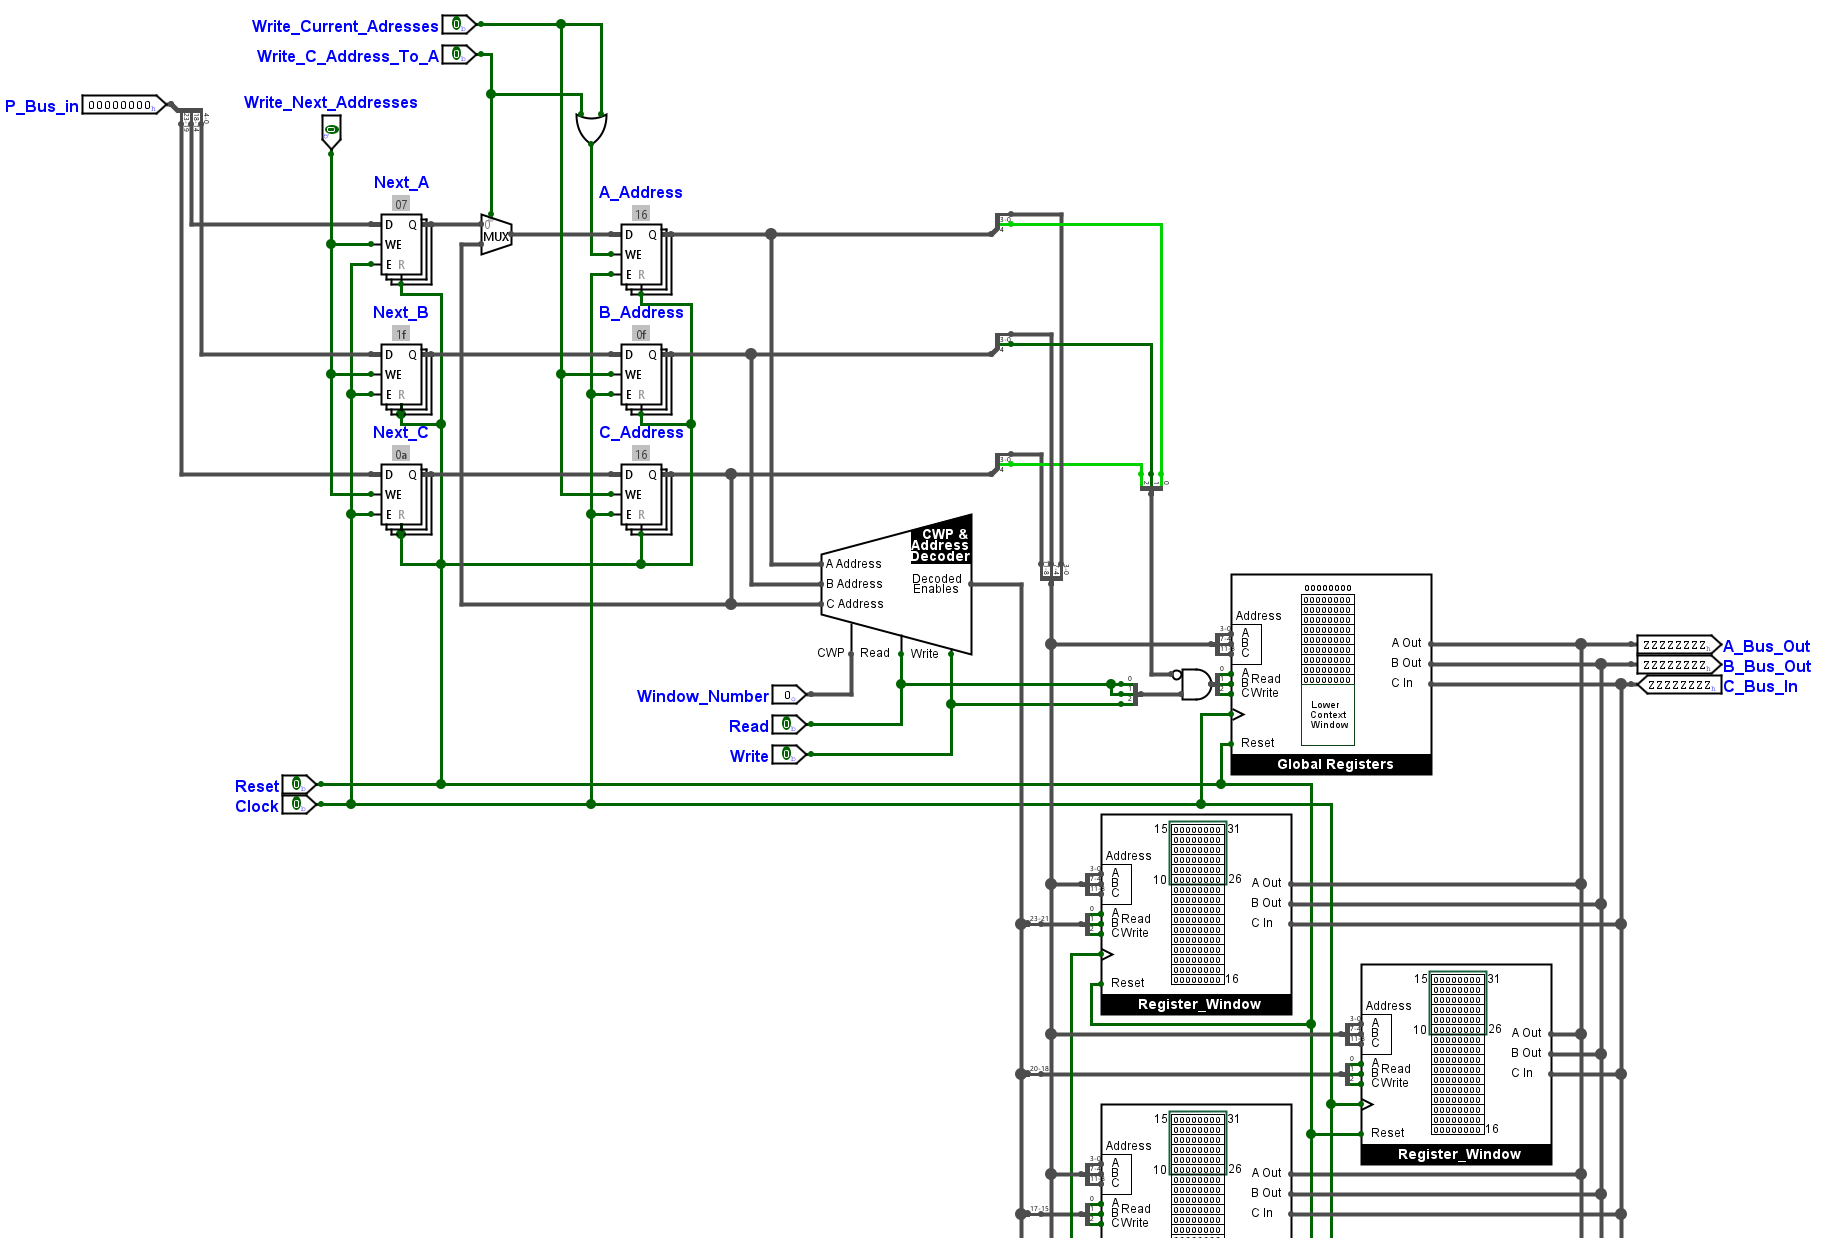
\includegraphics[width=0.75\linewidth]{Logisim/registerFile.png}
    \caption{Arquivo de registradores no Logisim}
    \label{fig:RegisterFile}
\end{figure}
A figura \ref{fig:RegisterFile} mostra uma parte do circuito to arquivo de registradores. A parte que não é mostrada é apenas a repetição dos 8 registradores locais. Algumas partes do circuito foram separadas em componentes próprios para simplificar a construção do modelo e melhorar o entendimento visual.

No RISC original, há 7 \textit{latches} para armazenar os endereços durante as diversas fases da \textit{pipeline}. No entanto, foi possível reproduzir a mesma funcionalidade utilizando apenas 6 \textit{flip-flops}. Destes, 3 armazenam a instrução que está sendo lida da memória, enquanto os outros 3 armazenam os endereços que estão sendo executados.

Em instruções de \textit{store}, o endereço C precisa ser passado para o endereço A, pois ele contém o registrador com a informação que deve ser gravada. Esta informação, por sua vez, deve ser passada como parâmetro para o deslocador. Para a passagem do endereço C para o endereço A, a saída do endereço C que está em execução é conectada à entrada do endereço A em execução através de um multiplexador.
\begin{figure}[H]
    \centering
    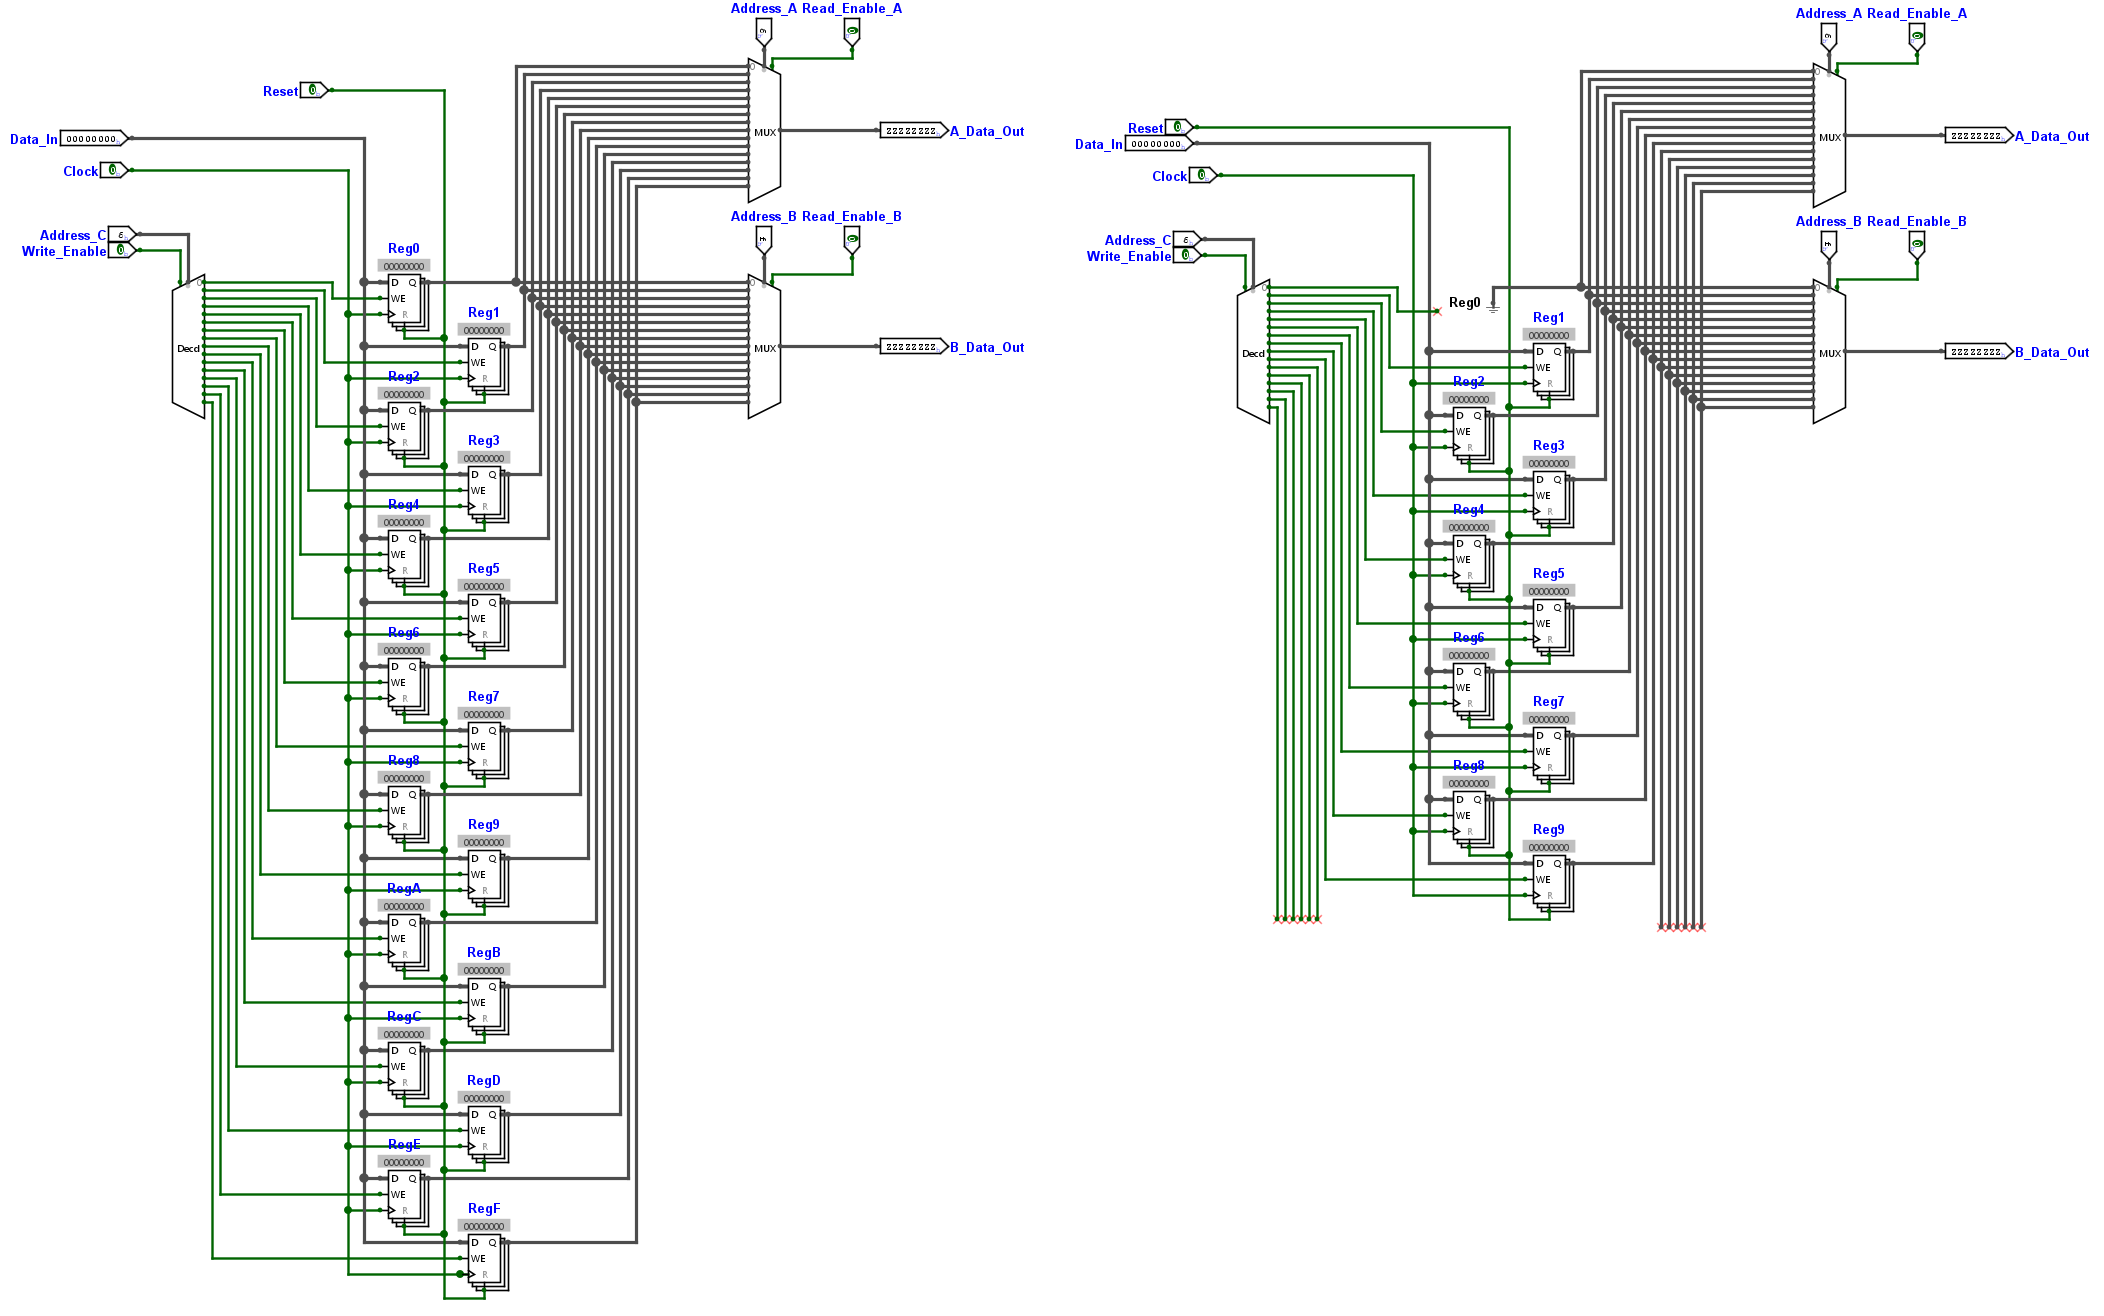
\includegraphics[width=0.75\linewidth]{Logisim/windowCells.png}
    \caption{À direita, uma célula de registradores locais; À esquerda, a célula contendo os registradores globais}
    \label{fig:windowCells}
\end{figure}
A figura \ref{fig:windowCells} mostra os circuitos de uma janela de registradores e os registradores globais. O circuito da janela recebe os 4 bits menos significativos dos endereços, que são utilizados em decodificadores e multiplexadores para a seleção dos registradores que serão lidos e escritos.

Para a seleção de qual registrador está sendo escrito, foi utilizado um decodificador que, ao receber o endereço e o sinal de escrita, ativa o pino de leitura de um dos 16 registradores da janela. Para a leitura de dados, foram utilizados 2 multiplexadores, um para cada barramento de leitura. Cada entrada dos multiplexadores recebe um registrador diferente e, ao receber o sinal de leitura com o endereço, a informação do registrador selecionado é retornada pelo componente. Caso não haja sinal de leitura, a conexão fica em alta impedância, similar a um \textit{buffer tri-state}, o que permite conectar a saída de várias janelas nos barramentos A e B sem criar curtos.

Para a criação dos registradores globais foi reutilizado o layout do circuito da janela, porém os 6 últimos registradores foram removidos por serem os registradores locais da janela abaixo, enquanto o primeiro registrador foi substituído por uma conexão terra na saída, retornando sempre 0. Será mostrado depois que os sinais pros registradores da janela anterior ainda são passados para esse componente, porém, por não haver nenhuma conexão interna, nenhum dado é gravado ou retornado neste componente quando isso acontece.

\begin{figure}[H]
    \centering
    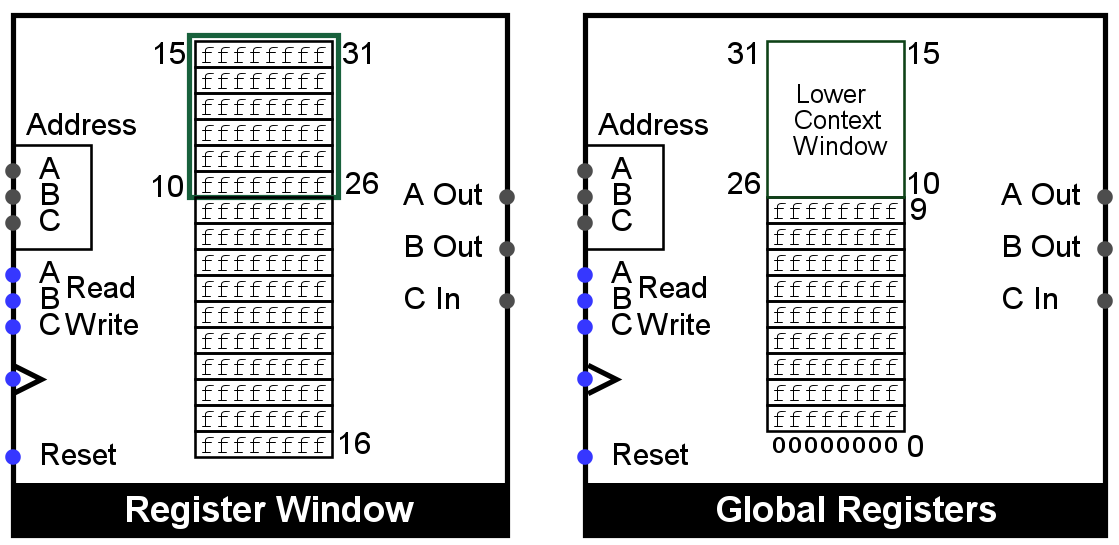
\includegraphics[width=0.5\linewidth]{Logisim/windowCellsPack.png}
    \caption{Pacotes das células locais e globais das janelas de registradores.}
    \label{fig:windowCellsPack}
\end{figure}
Os pacotes dos componentes ficaram similares. À esquerda, o componente recebe os três endereços dos registradores sendo usados pela instrução atual. Abaixo dos endereços, há três sinais de leitura e escrita, que só se ativam na janela em uso. À direita, estão as conexões de troca de dados: as saídas nos barramentos A e B, e a entrada no barramento C. No centro, é possível ver o valor de todos os registradores, com alguns endereços à direita (se for a janela atual) e à esquerda (se for a janela inferior), para ajudar na localização dos registradores compartilhados entre janelas.  
\begin{figure}[H]
    \centering
    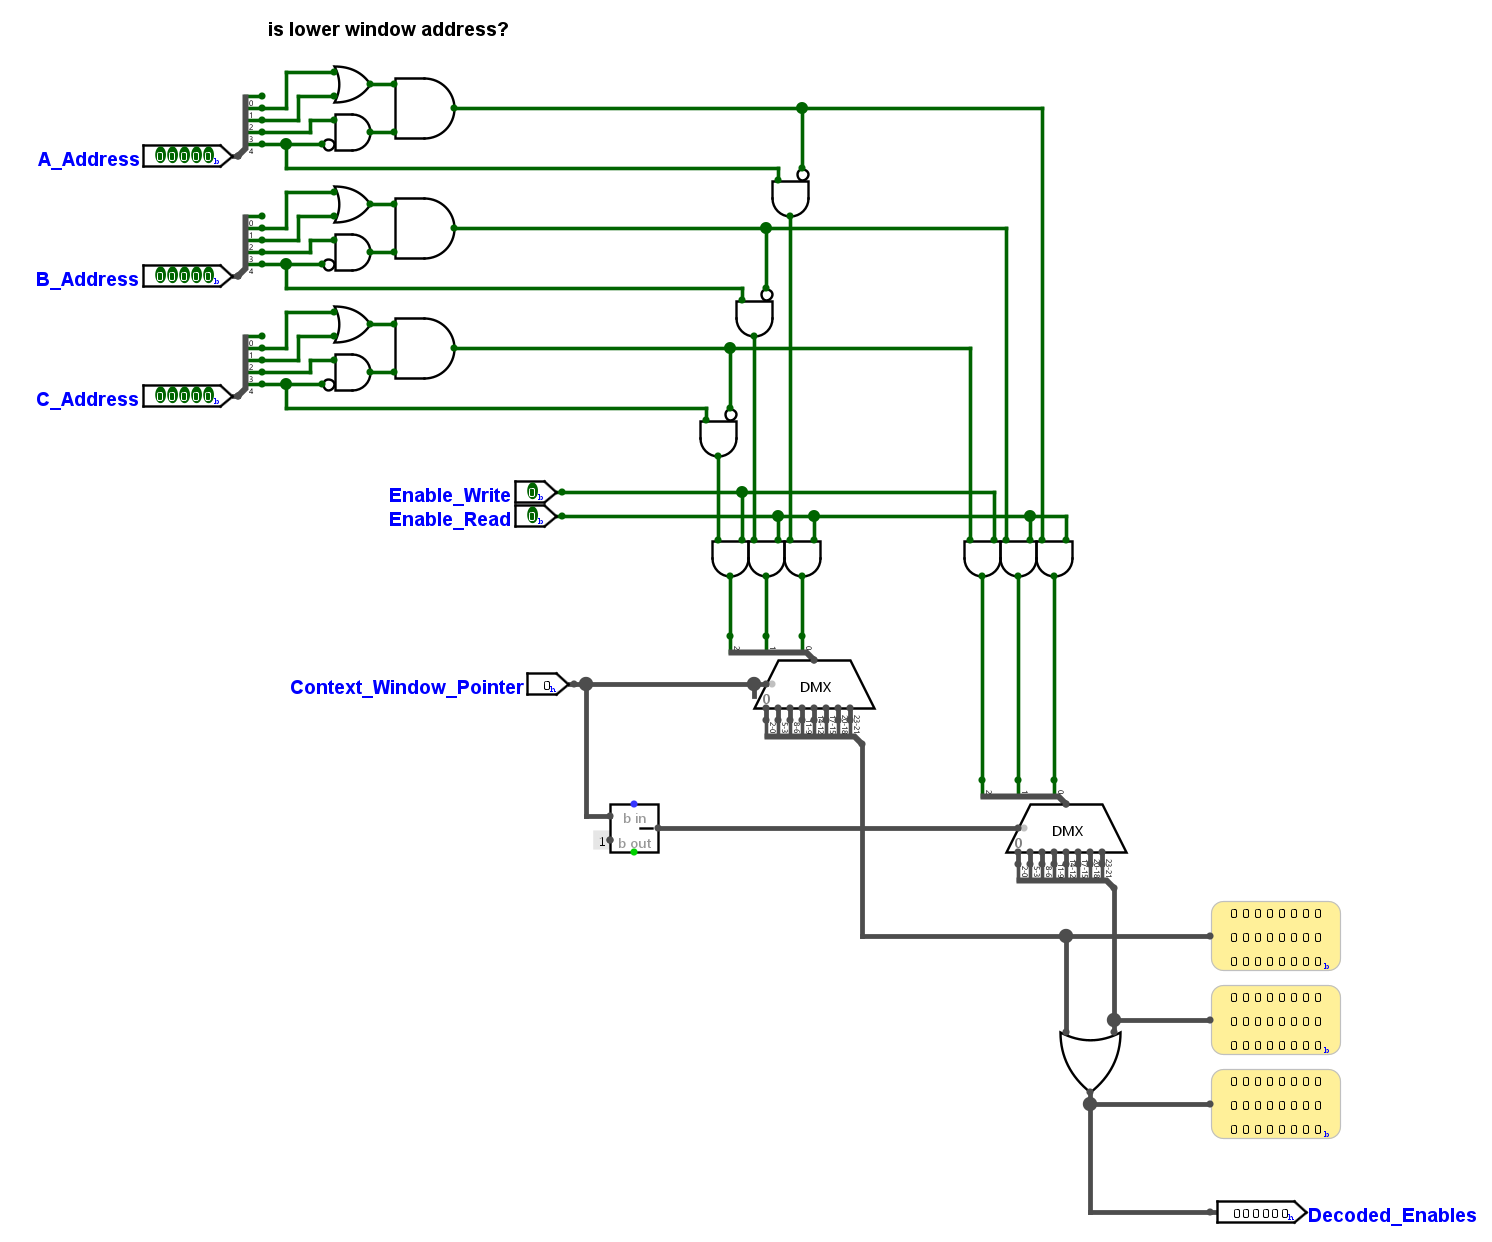
\includegraphics[width=0.75\linewidth]{cwpDecoder.png}
    \caption{Decodificador de endereço e do ponteiro da janela atual no Logisim}
    \label{fig:cwpDecoder}
\end{figure}
A figura \ref{fig:cwpDecoder} mostra o circuito do decodificador de endereços. Este componente recebe cada um dos endereços na instrução em execução e o número de janela, e retorna sinais controle para a janela que esta em atividade.  Caso o endereço esteja abaixo de 10, é um endereço global e não ativa nenhuma das janelas. Caso o endereço esteja entre 10 e 15, o sinal de controle vai para a janela que esta abaixo da janela atual. Caso seja entre 16 e 31 então o sinal de controle vai para a janela atual. 

Note que na figura \ref{fig:RegisterFile}, os sinais de controle para os registradores globais não passam pelo decodificador. Para ativar os registradores globais, é necessário apenas verificar se o bit mais significativo é 0. Caso seja 0, o registrador sendo manipulado é ou o local da janela anterior ou um dos globais. Como no componente de registradores globais as posições dos registradores locais não estão conectadas a nada, podemos enviar sinais de controle a este componente sem nos preocupar com a escrita simultânea em alguma janela local.
\begin{figure}[H]
    \centering
    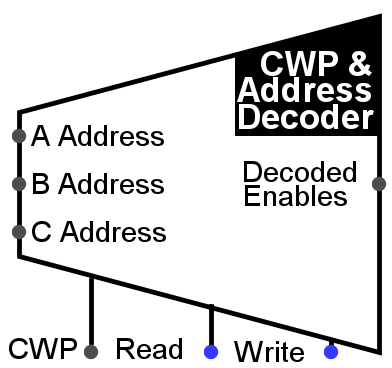
\includegraphics[width=0.25\linewidth]{Logisim/cwpDecoderPack.png}
    \caption{Pacote do decodificador de endereço e do ponteiro da janela atual}
    \label{fig:cwpDecoderPack}
\end{figure}
O Pacote do circuito possui um formato similar ao de um de-multiplexador. A entrada dos endereços fica à esquerda enquanto a saída dos sinais de controle para cada janela fica à direita. Em baixo do componente temos a entrada do número de janela atual(CWP) e dos sinais de leitura e escrita.
\begin{figure}[H]
    \centering
    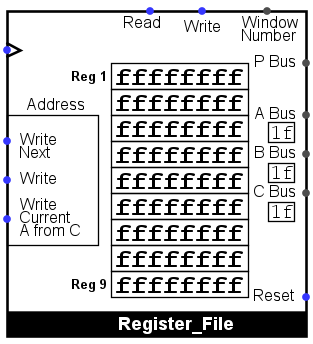
\includegraphics[width=0.25\linewidth]{Logisim/registerFilePack.png}
    \caption{Pacote do arquivo de registradores no Logisim}
    \label{fig:registerFilePack}
\end{figure}
Por fim, temos o pacote que engloba o arquivo de registradores, similar ao componente de janelas individuais, com os registradores globais no centro. Nas entradas e saídas dos barramentos A, B e C à direita, foram adicionados textos exibindo os endereços dos registradores utilizados. Há uma entrada do barramento P acima dos outros barramentos, usada para obter os endereços dos registradores da instrução lida. Acima do componente, temos a entrada do número de janela e os sinais de controle para leitura e escrita dos dados armazenados. À esquerda, encontram-se os sinais de controle para a escrita de endereços: os próximos endereços, os endereços da instrução em execução e a escrita do endereço C no A.

\subsubsection{Controlador de Janela}
\begin{figure}[H]
    \centering
    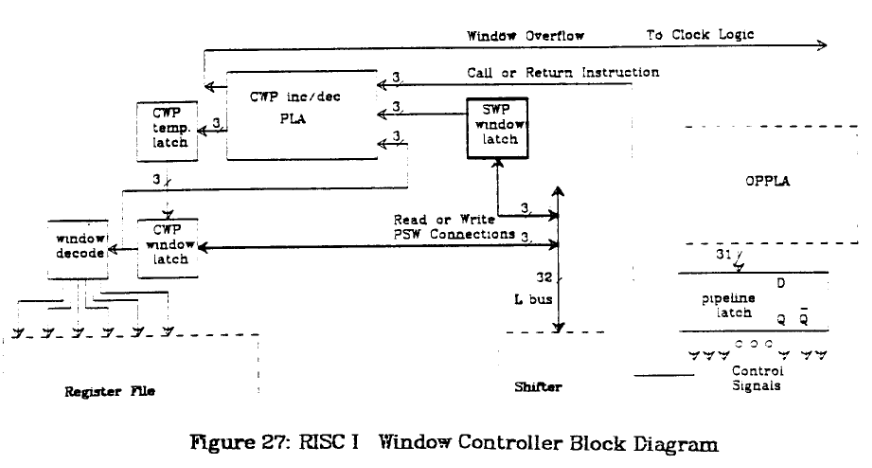
\includegraphics[width=0.75\linewidth]{Original/windowControllerPeek.png}
    \caption{Controlador de janela\cite{peek_vlsi_1983}.}
    \label{fig:windowControllerPeek}
\end{figure}
O controlador de janela original (figura \ref{fig:windowControllerPeek}) serve para guardar não só o número da janela atual, mas também o menor número de janela que foi salvo para poder ser usado no tratamento de \textit{overflows} de janela. Uma diferença na implementação realizada no Logisim foi que o número de janela aumenta em instruções de chamada e diminui em instruções de retorno. Isso foi feito para ficar mais alinhado com a ideia de uma pilha, além de fazer um pouco mais de sentido começar no 0 e a cada chamada aumentar o número. Esta modificação não gerou nenhuma diferença na funcionalidade da arquitetura, mas caso seja um problema futuro, pode ser facilmente revertido com poucas alterações.

Os valores dos registradores do número atual e do salvo da janela são passados para o barramento L durante toda fase 3n para poderem ser lidos pela palavra do processador. Ao executar uma instrução "PUTPSW", os valores dos números de janela são atualizados. Esta é a única forma de atualizar o número de janela salvo e essa instrução é executada durante rotinas de tratamento de \textit{overflow} de janela.

No controlador de janela original, há um decodificador embutido que transforma o número binário em um fio para cada janela, porém como mostrado na seção \ref{cap:registerFile}, essa decodificação ocorre dentro do arquivo de registradores, então foi removido da implementação no simulador. Para o cálculo de acréscimo e decremento de janela foi utilizados componentes subtratores e somadores conectados a um multiplexador para a seleção da operação. Finalmente foi utilizado um componente de comparação para a detecção de \textit{overflow} de janelas.

\begin{figure}[H]
    \centering
    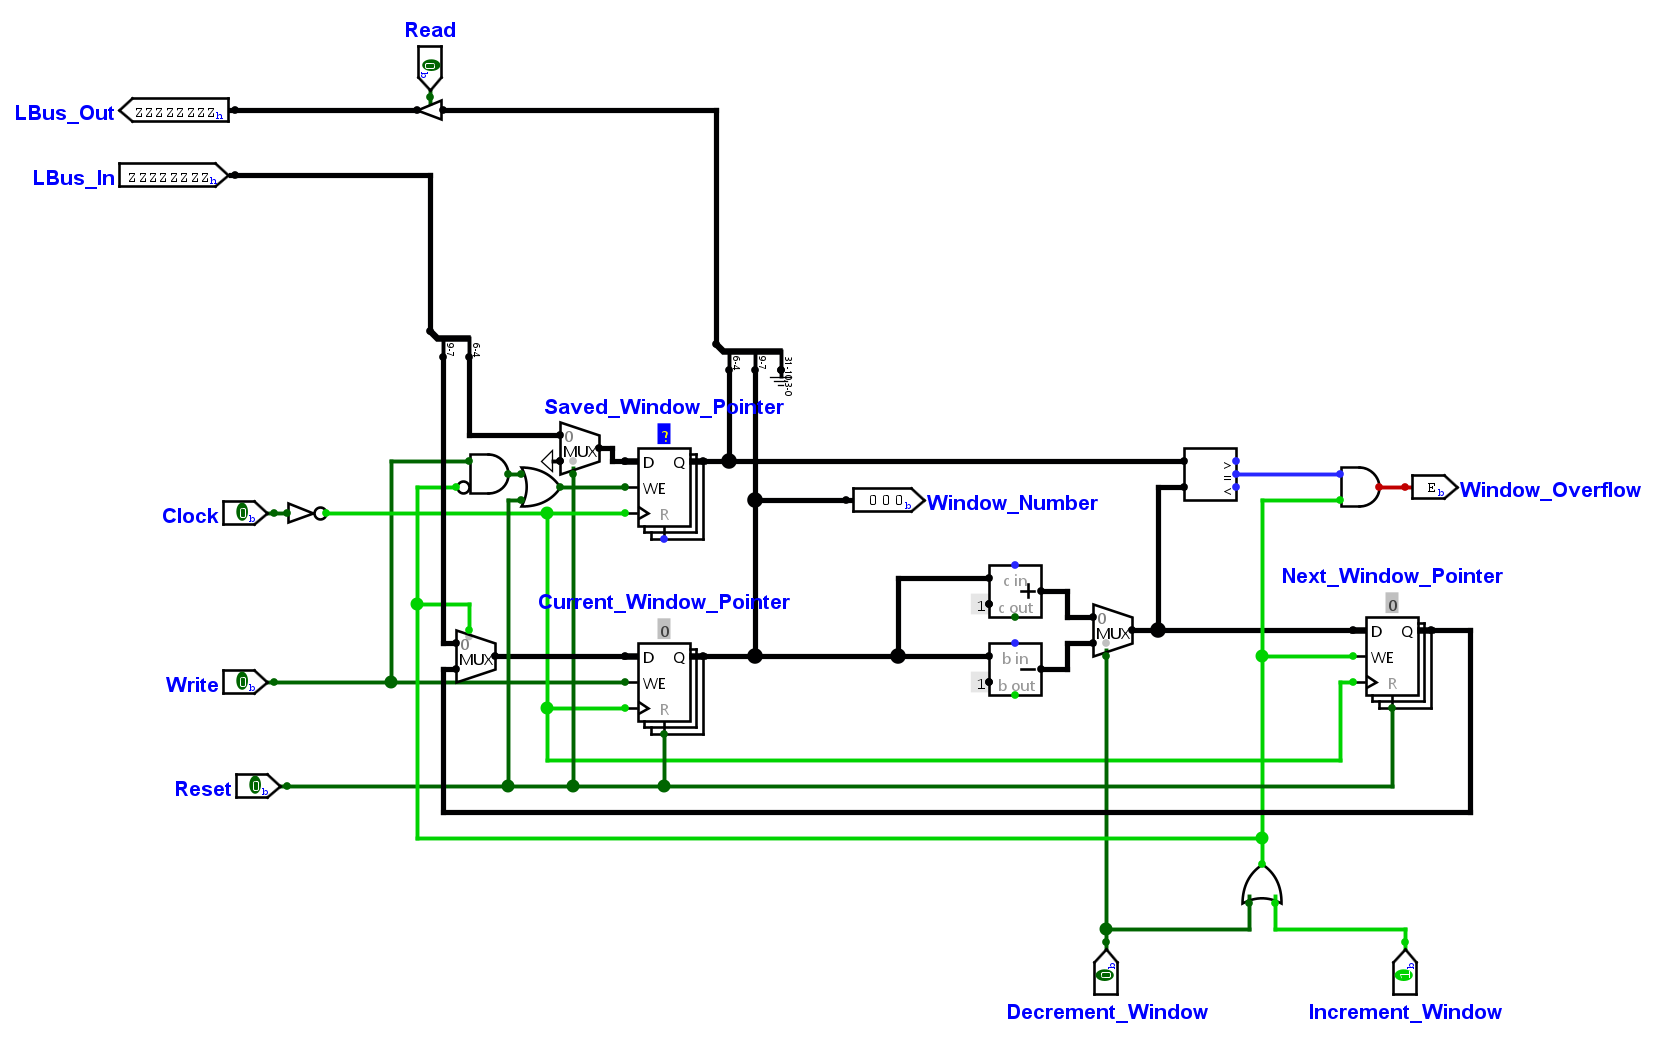
\includegraphics[width=0.75\linewidth]{Logisim/windowNumberController.png}
    \caption{Controlador de janela no Logisim}
    \label{fig:windowController}
\end{figure}
O pacote do contador possui os sinais de controle à direita junto com a conexão para o barramento L. A saída do número da janela fica a baixo e os sinais de \textit{reset} e \textit{clock} ficam à esquerda.
\begin{figure}[H]
    \centering
    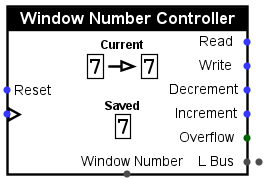
\includegraphics[width=0.25\linewidth]{Logisim/Pacote do Controlador de Janela no Logisim.png}
    \caption{Pacote do controlador de janela no Logisim}
    \label{fig:windowControllerPack}
\end{figure}
\subsection{Palavra de Estado do Processador}
A palavra de estado do processador precisa indicar duas coisas, os códigos de condição, que são retornados pela ULA, e os números de janela atual e salva. Na especificação original é utilizada uma palavra inteira(32 bits), mesmo que a informação salva ocupe apenas 10 desses bits, logo os outros 22 bits podem ser definidos pelo usuário ao utilizar a instrução "PUTPSW". 

O trabalho de Peek não detalha a implementação deste componente, então foi realizada a implementação a partir das especificações necessárias para seu funcionamento. Um registrador de 32 bits se conecta a entrada e saída para barramento L, assim pode ser utilizado nas instruções que modificam ou leiam seu valor, além de poder se comunicar com o registrador de número de janela. 

Quando a ULA realiza uma operação e a \textit{flag} para mudar códigos de condição(SCC) esta ativa, o código CNZV é gravado no registrador. O funcionamento da \textit{flag} SCC será explicada em mais detalhe no capítulo \ref{cap:controller}, mas podemos dizer que ela é gravada durante a busca de instrução e transmitida para o PSW durante a fase 3n. Nessa implementação, o número de janela é apenas gravado durante a ativação da \textit{flag} SCC. Caso a instrução em execução seja "PUTPSW", esta grava o seu valor durante a fase 2n. 
\begin{figure}[H]
    \centering
    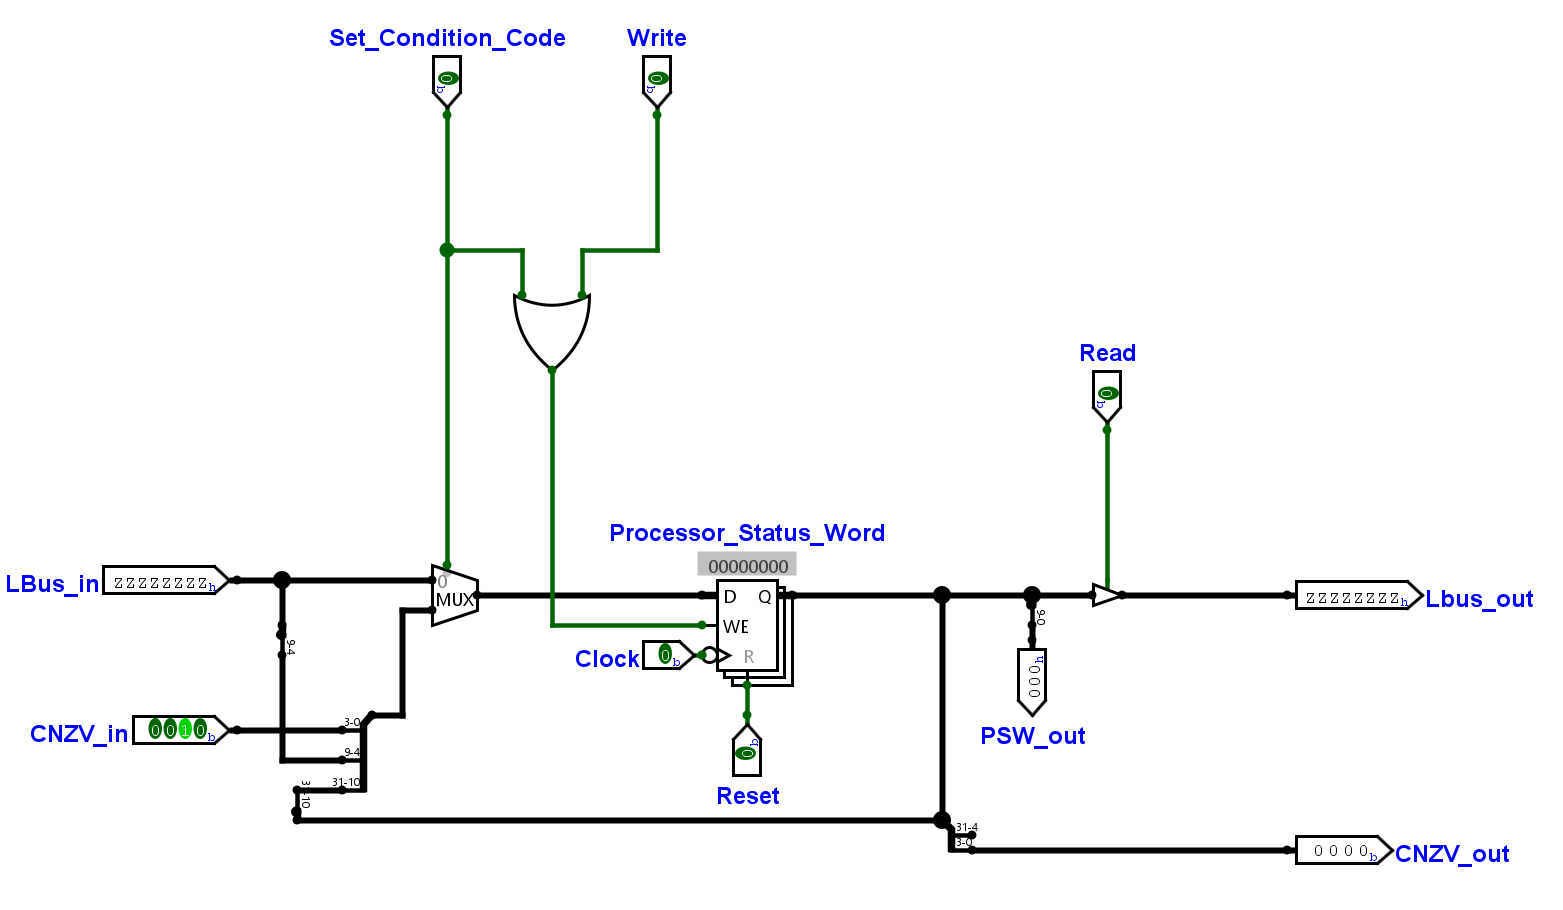
\includegraphics[width=0.75\linewidth]{Logisim/psw.png}
    \caption{Registrador de palavra de estado do processador no Logisim}
    \label{fig:psw}
\end{figure}
 O pacote do PSW possui sua conexão com o barramento L à esquerda, e o CNZV à direita. sinais de controle foram deixados em ambos os lados para manter o componente mais compacto. Adicionalmente, pela importância de seu valor, foi adicionado um texto grande que fica logo acima de seu título.
\begin{figure}[H]
    \centering
    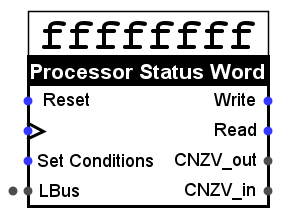
\includegraphics[width=0.25\linewidth]{Logisim/pswPack.png}
    \caption{Pacote do registrador de palavra de estado do processador no Logisim}
    \label{fig:pswPack}
\end{figure}
\subsection{Entrada e Saída}

O RISC~I pode se comunicar externamente com outros dispositivos através do barramento P, que se conecta diretamente a memória e dispositivos de entrada e saída. Além do barramento P, Alguns sinais de controle também devem ser utilizados para indicar quando uma leitura ou escrita devem ser realizadas, além de sinais para indicar qual é o tamanho do dado que esta sendo escrito. Finalmente, alguns sinais de temporização são utilizados para indicar quando o registrador de endereço da memória deve ser escrito, que ocorre durante as fases 1n e 3s. 
\begin{figure}[H]
    \centering
    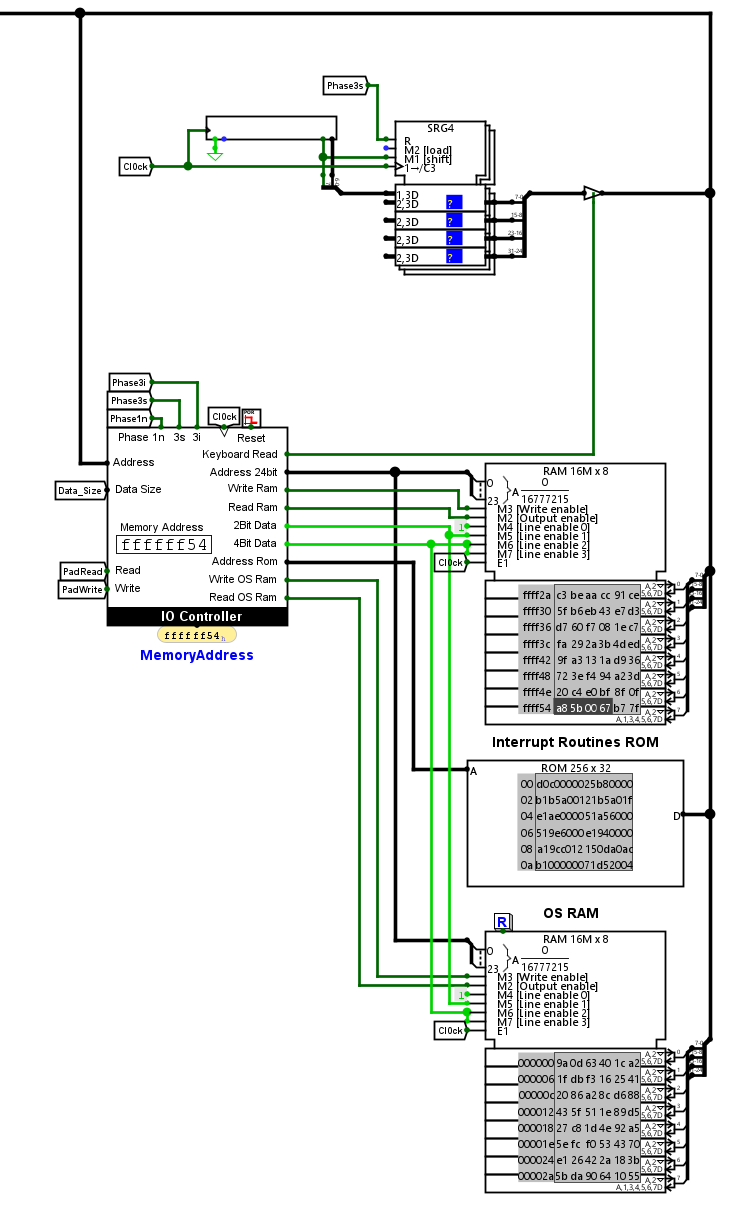
\includegraphics[width=0.5\linewidth]{Logisim/inputoutput.png}
    \caption{De cima para baixo: Dispositivo de entrada, memória RAM, ROM de rotinas de interrupção, RAM para o sistema operacional}
    \label{fig:iodevices}
\end{figure}

A Figura \ref{fig:iodevices} mostra a memória RAM, um dispositivo rudimentar para leitura de dados pelo usuário, uma ROM que armazena rotinas para tratamento de interrupções e uma memória RAM que é utilizada para armazenar resultados dessas rotinas. Um controlador foi criado para lidar com estes dispositivos. Este controlador armazena o endereço atual e o decodifica para selecionar qual dispositivo esta sendo utilizado. O registrador de endereço contido no controlador é atualizado durante a fase 1n no ciclo de busca de instrução e durante a fase 3s no ciclo de \textit{load} e \textit{store} e durante a fase 3i em interrupções. O circuito do controlador pode ser visto na Figura \ref{fig:IOController}.

\begin{figure}
    \centering
    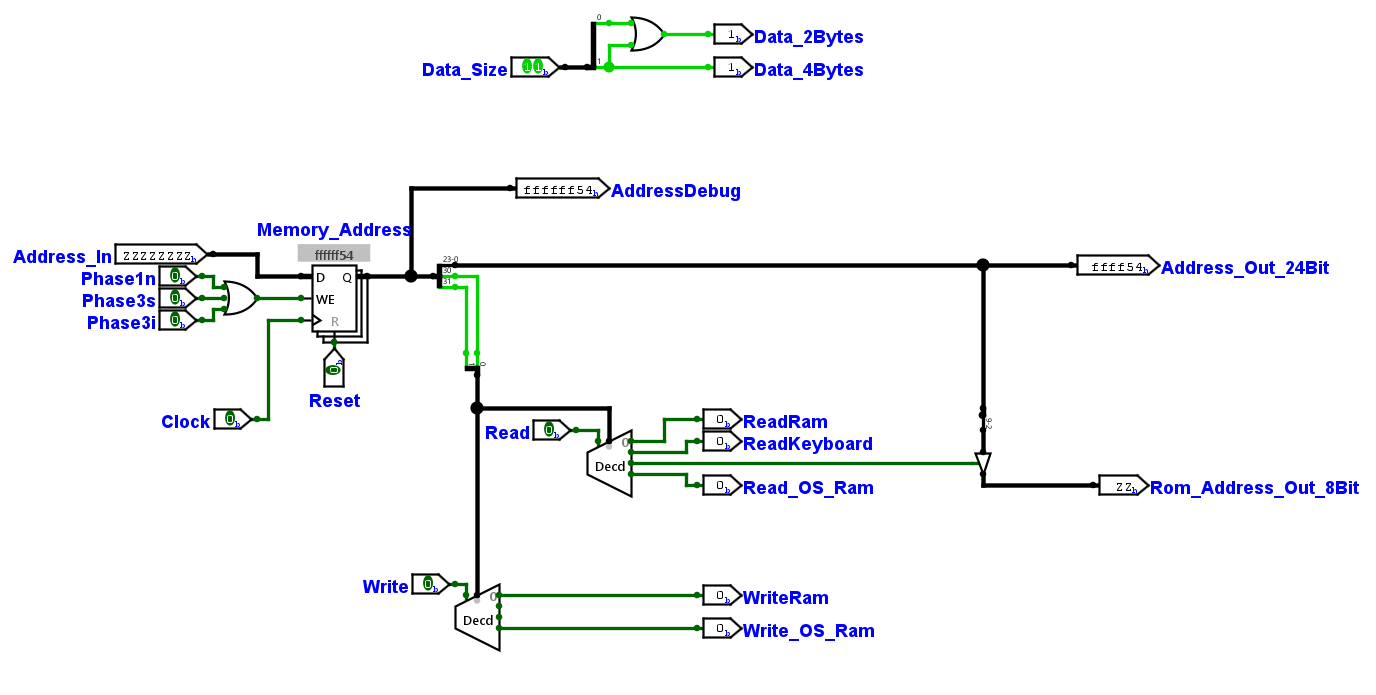
\includegraphics[width=0.75\linewidth]{Logisim/IOController.png}
    \caption{Controlador dos dispositivos de entrada e saída.}
    \label{fig:IOController}
\end{figure}

A memória RAM foi criada a partir de um componente pronto do Logisim, permitindo que programas compilados sejam carregados diretamente nela. Cada endereço possui 1 byte de informação e, a cada leitura, 4 endereços são lidos simultaneamente. Estes podem ser truncados e alinhados pelo \textit{dataIO} e pelo deslocador, caso a informação buscada seja menor que 32 bits. Durante a escrita, o endereço enviado para o registrador não precisa estar alinhado aos endereços das palavras completas (de 4 em 4), diferentemente da leitura. Além disso, um sinal do tamanho do dado sendo escrito deve ser enviado para a memória, podendo limitar a quantidade de endereços escritos a 1 ou 2 bytes.

A ROM é um componente simples, que recebe um endereço e devolve um valor. Caso o endereço esteja em alta impedância, então a saída também fica em alta impedância. Como só podem ser executadas instruções de \textit{load}, cada célula da ROM possui todos 32 bits, contendo a informação completa de cada instrução. Nessa versão do modelo, só há uma rotina para tratar problemas de \textit{overflow} e \textit{underflow} de janela, porém futuramente novas rotinas podem ser adicionas. Junto com a ROM uma segunda memória RAM foi adicionada, porém esta é de uso exclusivo para as rotinas. Assim que ocorre um \textit{overflow} de janela, a janela seguinte deve ser salva nesta RAM, podendo ser restaurada após a rotina de \textit{underflow}. Para funcionar corretamente é necessário que a o valor inicial da primeira célula desta memória seja 0xC0000000, o que indica que as janelas serão salvas logo após esta primeira célula. 

O dispositivo de entrada foi criado a partir de dois componentes do Logisim: um para coletar entrada do teclado em código ASCII e um registrador de deslocamento para armazenar os 4 últimos caracteres digitados (\textit{buffer} de entrada). A implementação deste dispositivo permite que dados escritos pelo usuário sejam lidos pelo processador sem a necessidade de alterar diretamente a memória RAM do sistema, oferecendo uma interface interativa. No entanto, a implementação possui várias limitações, como a falta de uma limpeza do \textit{buffer} após a leitura, a ausência de mecanismos para detectar quando não há novas informações para serem lidas e o tamanho limitado do \textit{buffer}. Este dispositivo pode ser aprimorado em versões futuras deste trabalho. No momento da criação deste relatório, ele serve mais como uma prova de conceito.

 \subsection{Controle}\label{cap:controller}

O circuito de controle (figura \ref{fig:controller1}) foi uma das partes mais diferentes da implementação original pela falta de informação no trabalho original. Apesar disso, foi possível replicar a mesma funcionalidade do original utilizando alguns dos conceitos que foram apresentados de forma geral. 

Foi utilizado um registrador que armazena a próxima instrução a ser executada na pipeline, que se conecta a 3 registradores referentes a instrução em execução, estes sendo o registrador do código da instrução(\textit{opcode}), um que armazena qual código de condição que esta sendo usado caso seja uma instrução "JMP", e o bit que diz se a ULA deve gravar no PSW.  Além desses registradores, também há um registrador CNZV que copia os códigos de condição da PSW.

\begin{figure}[H]
    \centering
    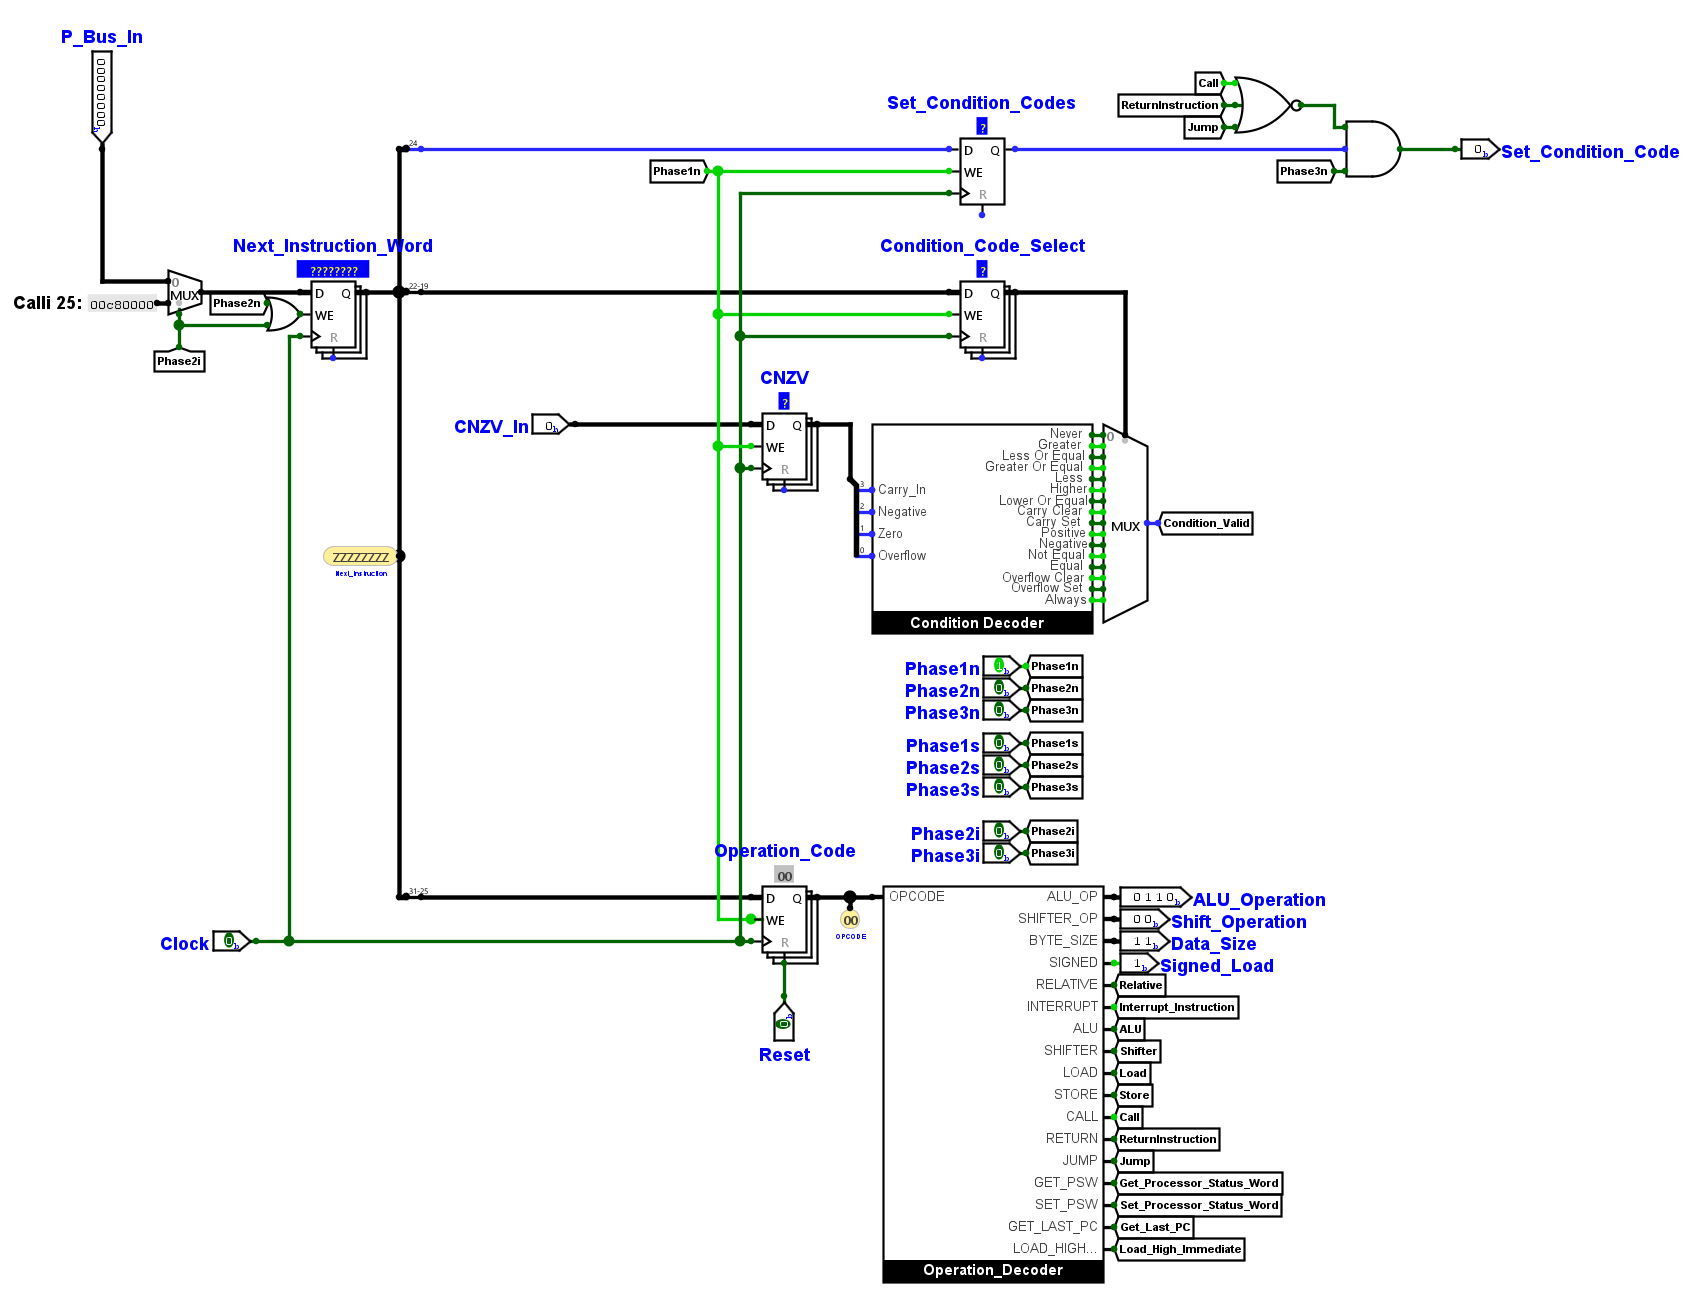
\includegraphics[width=0.75\linewidth]{Logisim/controller1.png}
    \caption{Registradores e decodificadores do controlador.}
    \label{fig:controller1}
\end{figure}

A informação armazenada pelos registradores passa então por uma decodificação em 2 partes. A primeira separa o \textit{opcode} em sinais que representam informações sobre qual tipo de instrução esta em execução. Esses sinais podem ser vistos no componente \textit{Operation Decoder}  na figura \ref{fig:controller1}, e as suas ativações podem ser vistas na tabela \ref{tab:opcodeDecoder}. Além da decodificação do \textit{opcode}, também é realizada a decodificação do código de condição, resultando em 16 sinais diferentes que são escolhidos por um multiplexador controlado pelo registrador de seleção do código de condição.

\begin{table}[!htp]\centering
\scriptsize
\begin{tabular}{lccccccccccccccccccc}\toprule
&Entrada &\multicolumn{6}{c}{Parâmetros} &\multicolumn{11}{c}{Instruções} \\\cmidrule{1-19}
Mnemonico & OPCODE[6..0] & \rotatebox{90}{ALU\_OP[3..0]} & \rotatebox{90}{SHIFTER\_OP[1..0]} & \rotatebox{90}{BYTE\_SIZE[1..0]} & \rotatebox{90}{SIGNED} & \rotatebox{90}{RELATIVE} & \rotatebox{90}{INTERRUPT} & \rotatebox{90}{ALU} & \rotatebox{90}{SHIFTER} & \rotatebox{90}{LOAD} & \rotatebox{90}{STORE} & \rotatebox{90}{CALL} & \rotatebox{90}{RETURN} & \rotatebox{90}{JUMP} & \rotatebox{90}{GET\_PSW} & \rotatebox{90}{SET\_PSW} & \rotatebox{90}{GET\_LAST\_PC} & \rotatebox{90}{LOAD\_HIGH\_IMMEDIATE} \\
\midrule
CALLI &0000XXX &0110 &00 &11 &1 &0 &1 &0 &0 &0 &0 &1 &0 &0 &0 &0 &0 &0 \\
CALL &000100X &0110 &00 &11 &1 &0 &0 &0 &0 &0 &0 &1 &0 &0 &0 &0 &0 &0 \\
JMP &000101X &0110 &00 &11 &1 &0 &0 &0 &0 &0 &0 &0 &0 &1 &0 &0 &0 &0 \\
CALLR &000110X &0110 &00 &11 &1 &1 &0 &0 &0 &0 &0 &1 &0 &0 &0 &0 &0 &0 \\
JMPR &000111X &0110 &00 &11 &1 &1 &0 &0 &0 &0 &0 &0 &0 &1 &0 &0 &0 &0 \\
SLL &0010X0X &0110 &00 &11 &1 &0 &0 &0 &1 &0 &0 &0 &0 &0 &0 &0 &0 &0 \\
GETPSW &0010X1X &0110 &00 &11 &1 &0 &0 &0 &0 &0 &0 &0 &0 &0 &1 &0 &0 &0 \\
SRL &001100X &0110 &01 &11 &1 &0 &0 &0 &1 &0 &0 &0 &0 &0 &0 &0 &0 &0 \\
PUTPSW &001101X &0110 &00 &11 &1 &0 &0 &0 &0 &0 &0 &0 &0 &0 &0 &1 &0 &0 \\
SRA &00111XX &0110 &10 &11 &1 &0 &0 &0 &1 &0 &0 &0 &0 &0 &0 &0 &0 &0 \\
ILLEGAL &01000XX &0110 &00 &11 &1 &0 &0 &0 &0 &0 &0 &0 &0 &0 &0 &0 &0 &0 \\
LDBU &0100100 &0110 &00 &00 &0 &0 &0 &0 &0 &1 &0 &0 &0 &0 &0 &0 &0 &0 \\
LDRBU &0100101 &0110 &00 &00 &0 &1 &0 &0 &0 &1 &0 &0 &0 &0 &0 &0 &0 &0 \\
LDBS &0100110 &0110 &00 &00 &1 &0 &0 &0 &0 &1 &0 &0 &0 &0 &0 &0 &0 &0 \\
LDRBS &0100111 &0110 &00 &00 &1 &1 &0 &0 &0 &1 &0 &0 &0 &0 &0 &0 &0 &0 \\
LDW &01010X0 &0110 &00 &11 &1 &0 &0 &0 &0 &1 &0 &0 &0 &0 &0 &0 &0 &0 \\
LDRW &01010X1 &0110 &00 &11 &1 &1 &0 &0 &0 &1 &0 &0 &0 &0 &0 &0 &0 &0 \\
LDSU &0101100 &0110 &00 &01 &0 &0 &0 &0 &0 &1 &0 &0 &0 &0 &0 &0 &0 &0 \\
LDRSU &0101101 &0110 &00 &01 &0 &1 &0 &0 &0 &1 &0 &0 &0 &0 &0 &0 &0 &0 \\
LDSS &0101110 &0110 &00 &01 &1 &0 &0 &0 &0 &1 &0 &0 &0 &0 &0 &0 &0 &0 \\
LDRSS &0101111 &0110 &00 &01 &1 &1 &0 &0 &0 &1 &0 &0 &0 &0 &0 &0 &0 &0 \\
STS &01100X0 &0110 &00 &01 &1 &0 &0 &0 &0 &0 &1 &0 &0 &0 &0 &0 &0 &0 \\
STRS &01100X1 &0110 &00 &01 &1 &1 &0 &0 &0 &0 &1 &0 &0 &0 &0 &0 &0 &0 \\
STB &01101X0 &0110 &00 &00 &1 &0 &0 &0 &0 &0 &1 &0 &0 &0 &0 &0 &0 &0 \\
STRB &01101X1 &0110 &00 &00 &1 &1 &0 &0 &0 &0 &1 &0 &0 &0 &0 &0 &0 &0 \\
STW &0111XX0 &0110 &00 &11 &1 &0 &0 &0 &0 &0 &1 &0 &0 &0 &0 &0 &0 &0 \\
STRW &0111XX1 &0110 &00 &11 &1 &1 &0 &0 &0 &0 &1 &0 &0 &0 &0 &0 &0 &0 \\
AND &10000XX &0001 &00 &11 &1 &0 &0 &1 &0 &0 &0 &0 &0 &0 &0 &0 &0 &0 \\
XOR &10001XX &0010 &00 &11 &1 &0 &0 &1 &0 &0 &0 &0 &0 &0 &0 &0 &0 &0 \\
OR &1001XXX &0011 &00 &11 &1 &0 &0 &1 &0 &0 &0 &0 &0 &0 &0 &0 &0 &0 \\
SUB &101000X &0100 &00 &11 &1 &0 &0 &1 &0 &0 &0 &0 &0 &0 &0 &0 &0 &0 \\
SUBC &101001X &0100 &00 &11 &1 &0 &0 &1 &0 &0 &0 &0 &0 &0 &0 &0 &0 &0 \\
SUBR &101010X &0101 &00 &11 &1 &0 &0 &1 &0 &0 &0 &0 &0 &0 &0 &0 &0 &0 \\
SUBCR &101011X &1100 &00 &11 &1 &0 &0 &1 &0 &0 &0 &0 &0 &0 &0 &0 &0 &0 \\
ADD &10110XX &0110 &00 &11 &1 &0 &0 &1 &0 &0 &0 &0 &0 &0 &0 &0 &0 &0 \\
ADDC &10111XX &0111 &00 &11 &1 &0 &0 &1 &0 &0 &0 &0 &0 &0 &0 &0 &0 &0 \\
RET &11000XX &0110 &00 &11 &1 &0 &0 &0 &0 &0 &0 &0 &1 &0 &0 &0 &0 &0 \\
RETI &11001XX &0110 &00 &11 &1 &0 &1 &0 &0 &0 &0 &0 &1 &0 &0 &0 &0 &0 \\
GETLPC &1101XXX &0110 &00 &11 &1 &0 &0 &0 &0 &0 &0 &0 &0 &0 &0 &0 &1 &0 \\
LDHI &111XXXX &0000 &00 &11 &1 &0 &0 &0 &0 &0 &0 &0 &0 &0 &0 &0 &0 &1 \\
\bottomrule
\end{tabular}
\caption{Tabela de decodificação de \textit{opcode}}\label{tab:opcodeDecoder}
\end{table}

Após a primeira parte da decodificação, vem a segunda parte, que combina os sinais gerados com os sinais das fases, gerando sinais compatíveis com os que cada componente individual recebe. Estes sinais e suas lógicas podem ser vistas na figura \ref{fig:controller2}.

\begin{figure}[H]
    \centering
    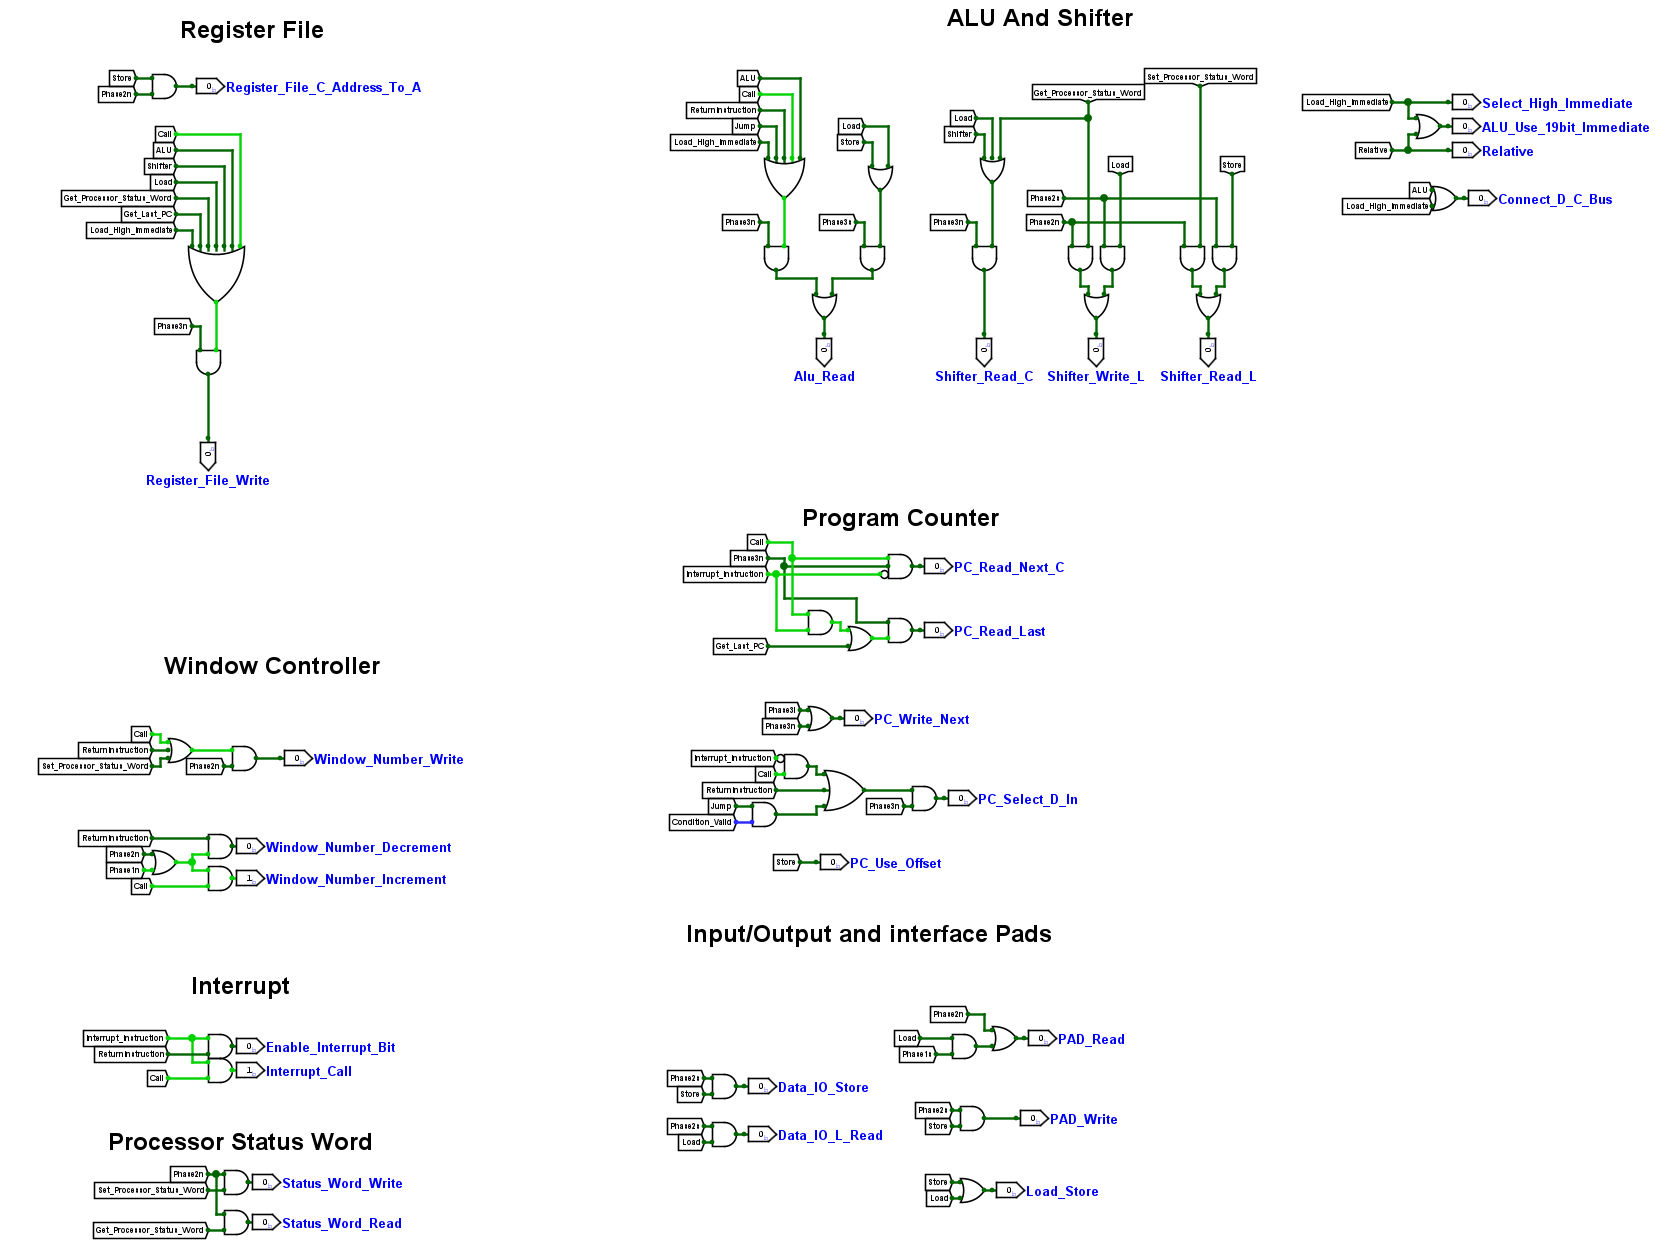
\includegraphics[width=0.75\linewidth]{Logisim/controller2.png}
    \caption{Geração dos sinais de controle finais.}
    \label{fig:controller2}
\end{figure}

No pacote do componente é possível ver a entrada de todas fases na parte superior, junto com o \textit{clock} e a entrada do barramento P. todas as saídas de controle ficaram nas laterais, junto com a entrada do CNZV na parte inferior esquerda, enquanto o \textit{reset} fica em baixo. Para ajudar na organização os sinais foram agrupados em casos onde eles controlam o mesmo componente. Os registradores que guardam informações da instrução em execução tem seu valor exposto.
\begin{figure}[H]
    \centering
    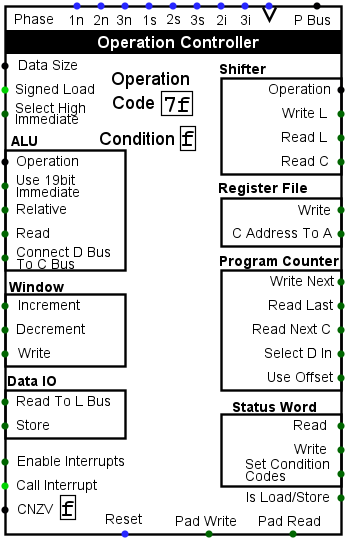
\includegraphics[width=0.25\linewidth]{Logisim/controllerPack.png}
    \caption{Pacote do controlador principal no Logisim}
    \label{fig:controllerPack}
\end{figure}

\subsection{Integração final}
Para a conexão de todos os componentes algumas regras foram seguidas. Todos sinais do controlador são passados para os componentes utilizando componentes de portal para manter a visualização do circuito mais limpa, e a mesma regra vale para todos os sinais de tempo que se conectam diretamente aos componentes. Conexões de barramento devem ficar explicitas, e sinais de controles gerado por componentes que não são o controle também ficam explicitas, como por exemplo o \textit{overflow} de janela. Um espaçamento mínimo foi dado para que os componentes não fiquem muito próximos, e qualquer conexão, quando possível, não pode passar sobre nenhuma outra. Componentes que tem seus valores gravados antes de serem lidos não precisam de sinal de \textit{reset}, os que precisam tem sua entrada de \textit{reset} conectada a um componente que gera um sinal positivo por x tempo toda vez que a simulação é reiniciada.

\begin{figure}[H]
    \centering
    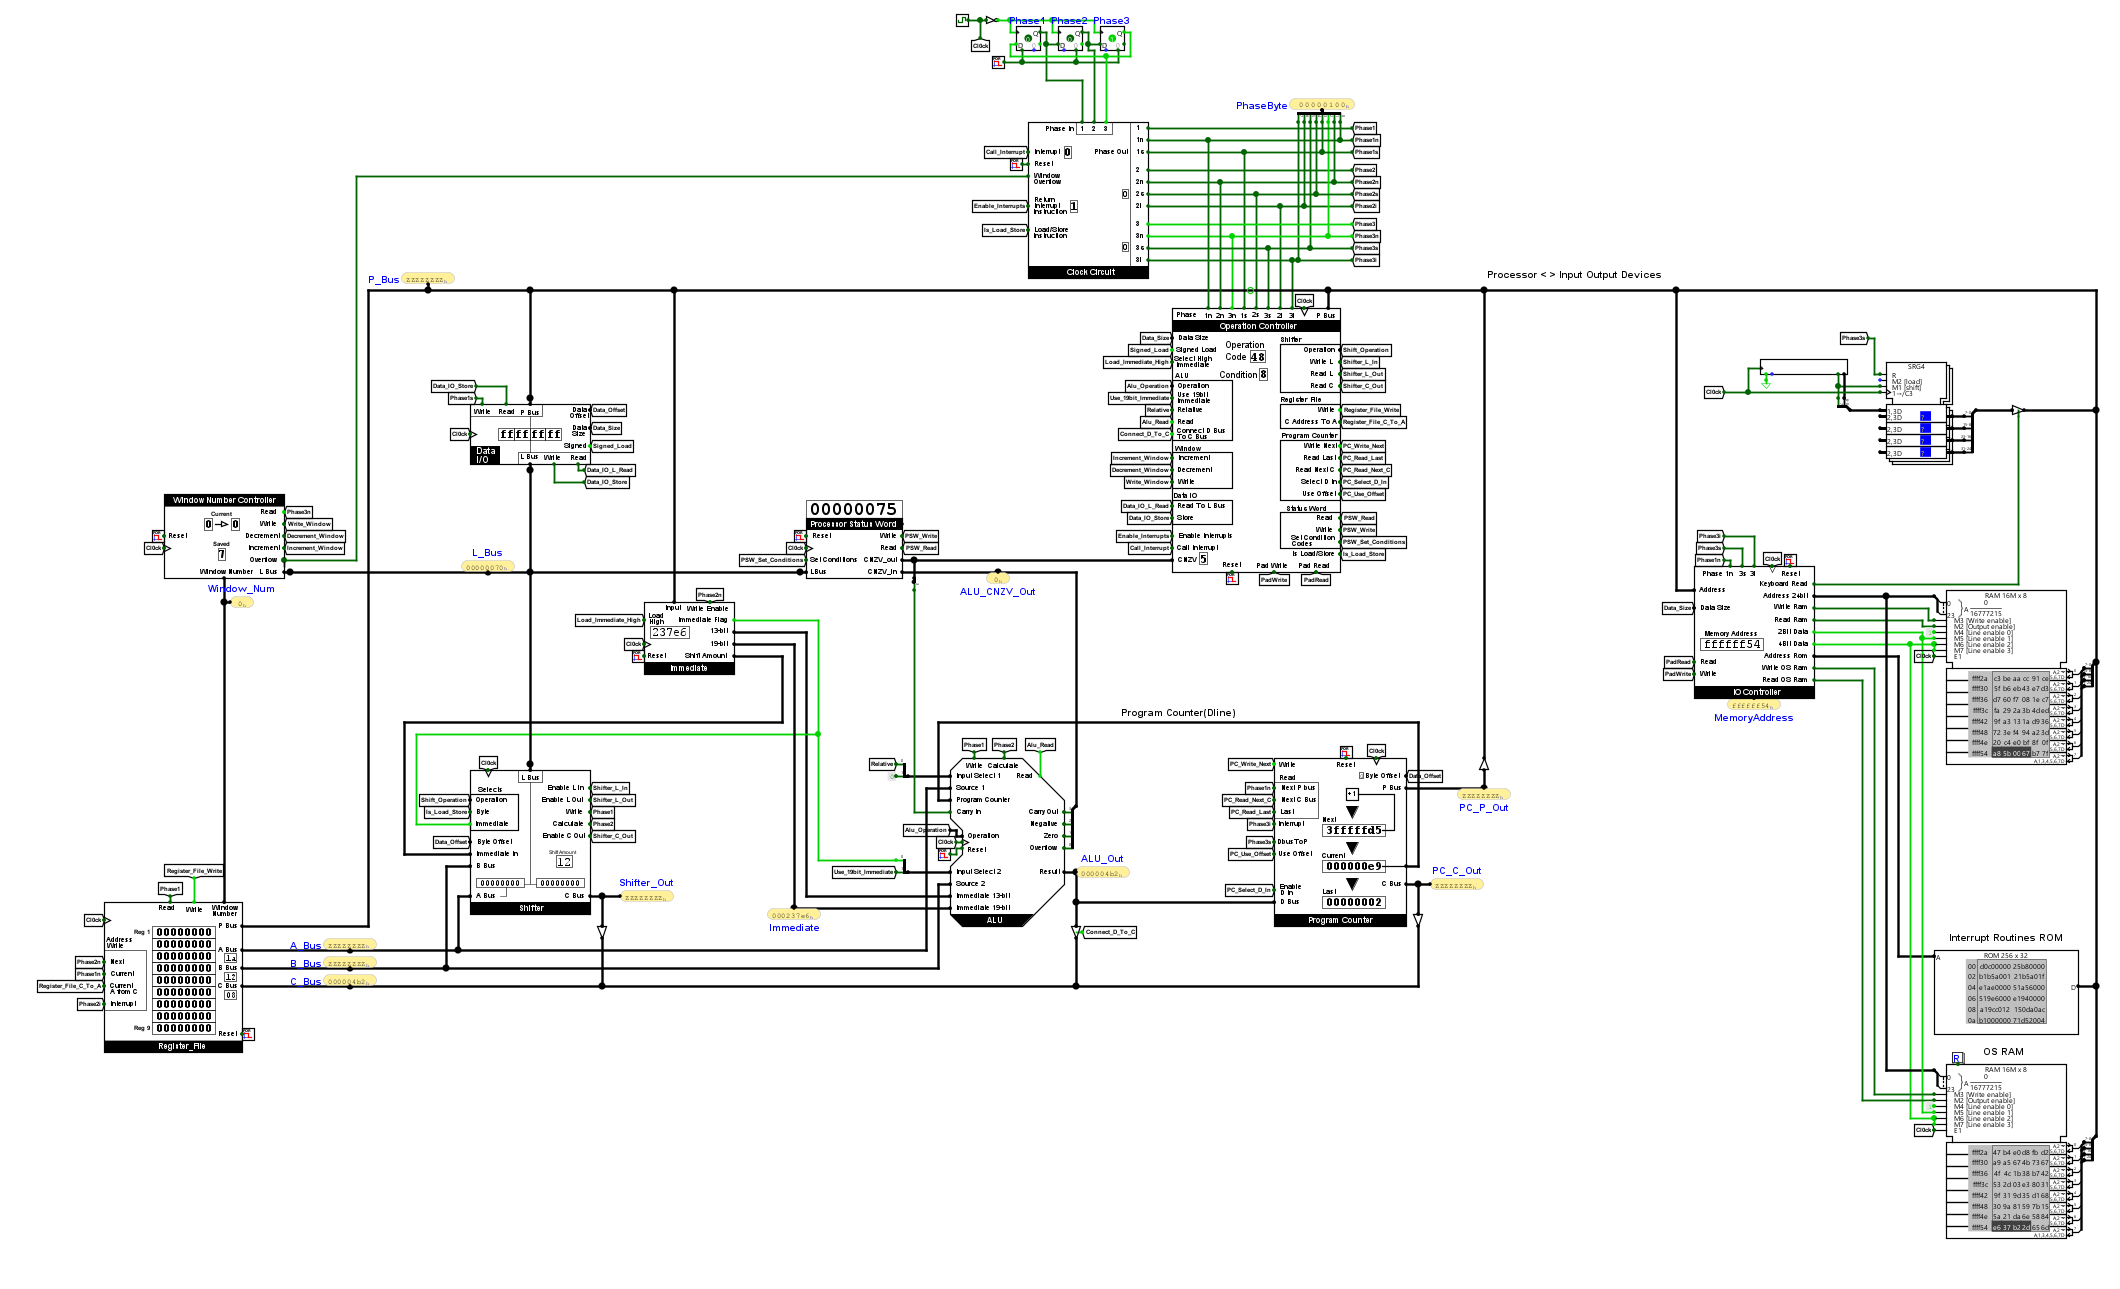
\includegraphics[width=1\linewidth]{Logisim/riscInternal.png}
    \caption{Circuito do RISC~I completo}
    \label{fig:internalCircuit}
\end{figure}
\section{Assembler}
\subsection{Funcionamento Geral}
Um assembler foi criado nesse trabalho para facilitar o trabalho de criação de programas para o modelo de simulação. A estrutura do código do assembly é bem simples, e seu funcionamento bem rudimentar, porém funcional. Ele funciona a partir de 6 fases: Leitura e divisão do código, remoção de espaços brancos e comentários, leitura e gravação de rótulos(\textit{labels}), leitura e gravação de palavras, tradução das instruções e geração da saída.

\subsubsection{Leitura e Divisão do Arquivo}
A primeira parte é bem simples. Primeiro, o arquivo é lido do sistema usando as classes \texttt{System.IO.File} e \texttt{System.IO.StreamReader}, guardando a informação lida em uma \textit{string}. Após essa leitura, o método \texttt{Assemble()} da classe do nosso \textit{assembler} é chamado, passando a string que foi lida e a largura de endereço e dados que definirá a formatação de saída.

\begin{lstlisting}
var fileContents = File.Open(targetFile, FileMode.Open);
var reader = new StreamReader(fileContents);
var input = reader.ReadToEnd();
string output = "";
try
{
    output = RiscAssembler.Assembler.Assemble(input, int.Parse(configSettings["bitWidth"]), int.Parse(configSettings["addressWidth"]));
}
\end{lstlisting}

Dentro do nosso método \texttt{Assemble()}, a \textit{string} da entrada é então dividida em uma lista de strings onde cada uma representa uma linha. Adicionalmente, é criado um vetor de \textit{uint} que representa a porção da memória que será enviada para o simulador, contendo todo o código compilado do nosso programa.

\begin{lstlisting}
private static readonly string[] separator = ["\r\n", "\r", "\n"];
[...]
public static string Assemble(string input, int bitWidth, int addressWidth)
{
    var lines = input.Replace("\t", "").Split(separator, StringSplitOptions.None);
    var memory = new uint[2 << addressWidth];
    var linesList = lines.ToList();
\end{lstlisting}

\subsubsection{Remoção de Espaços Brancos e comentários}

Após a divisão das linhas, estas são passadas para um método de limpeza que itera sobre cada linha removendo quaisquer comentários e linhas vazias.

\begin{lstlisting}
private static void RemoveCommentsAndBlankLines(List<string> lines)
{
    for (int currentLine = lines.Count - 1; currentLine >= 0 ; currentLine--)
    {
        var commentIndex = lines[currentLine].IndexOf("//");
        if (commentIndex >= 0) lines[currentLine] = lines[currentLine][0..(commentIndex)];
        if (lines[currentLine] == "")
        {
            lines.RemoveAt(currentLine);
        }
    }
}
\end{lstlisting}

\subsubsection{Leitura de Rótulos}
Os rótulos, ou \textit{labels}, são importantes para facilitar o trabalho de referenciar linhas especificas de código em outras. Ao declarar um rótulo, este fica vinculado a linha seguinte, que pode ser referênciada em outras linhas apenas chamando pelo nome do rótulo. Para declarar e chamar um rótulo, basta que ele seja colocado seguido de dois pontos(:). No assembler todos os rótulos são salvos em um dicionário onde a chave é o nome do rótulo o valor é o endereço onde a próxima linha de código será gravada.
\begin{lstlisting}
Dictionary<string, uint> labels = ExtractLabels(linesList);
[...]
private static Dictionary<string, uint> ExtractLabels(List<string> lines)
{
    Dictionary<string, uint> labels = [];
    for (int currentLine = 0; currentLine < lines.Count; currentLine++)
    {
        if (!lines[currentLine].StartsWith(':')) continue;
        labels.Add(lines[currentLine], (uint)currentLine << 2);
        lines.RemoveAt(currentLine);
        currentLine--;
    }
    return labels;
} 
\end{lstlisting}

\subsubsection{Leitura de Palavras}

Para a leitura de palavras, que correspondem às variáveis da nossa linguagem assembly, é realizado um processo semelhante ao da leitura de rótulos. A diferença é que não queremos apagar as linhas da nossa lista, pois estas serão gravadas na memória. É importante notar que o RISC~I suporta não apenas palavras (32 bits), mas também \textit{short} ou \textit{half} (16 bits) e byte (8 bits). No entanto, nesta versão do \textit{assembler}, não houve a necessidade de implementar esses tipos. Futuras versões poderão incluir a adição desse recurso, mas, por enquanto, o código contém apenas uma declaração desses tipos para futura implementação.


\begin{lstlisting}
Dictionary<string, uint> words = ExtractVariables(linesList);
[...]
private static Dictionary<string, uint> ExtractVariables(List<string> lines)
{
    Dictionary<string, uint> words = [];
    for (int currentLine = 0; currentLine < lines.Count; currentLine++)
    {
        var parts = lines[currentLine].Split(' ');
        switch (parts[0])
        {
            case ".word":
                words.Add(parts[1], (uint)currentLine << 2);
                break;
            case ".short":
            case ".half":
            case ".byte":
                throw new NotImplementedException();
        }
    }
    return words;
}
\end{lstlisting}

\subsubsection{Tradução das Instruções}

Esta é a parte mais longa e complexa do \textit{assembler}, porém segue um padrão básico para a tradução de cada parâmetro. Primeiro a linha é dividida em várias partes utilizando os caracteres em branco entre os parâmetros, e após isso cada parâmetro é decodificado e escrito na "memória" utilizando operações \textit{bitwise}.

\begin{lstlisting}
for (uint currentLine = 0, address = 0; currentLine < lines.Length; currentLine++, address++)
{
    var parts = lines[currentLine].Split(' ');
\end{lstlisting}
A tradução se inicia com um \textit{loop for} que itera sobre cada linha, dividindo a instrução em seus diversos parâmetros.

\begin{lstlisting}
if (parts[0].StartsWith('.'))
{
    if (parts[2].StartsWith('#'))
    {
        memory[address] = uint.Parse(parts[2][1..^0],hexStyle);
    }
    else if (parts[2].StartsWith(':'))
    {
        memory[address] = labels[parts[2]];
    }
    else                    
    {
        memory[address] = uint.Parse(parts[2],intStyle);
    }
    continue;
}
\end{lstlisting}
Após a separação, verifica-se se a linha começa com ".", significando que é uma declaração de uma variável. Caso seja, a terceira parte da linha pode ser um valor hexadecimal (começando com "\#"), um endereço de um rótulo (começando com ":") ou um inteiro. Este valor é então gravado no endereço de memória, e o resto do \textit{loop} é pulado para a leitura da próxima linha.

\begin{lstlisting}
if (parts[0][^1] == '*')
{
    parts[0] = parts[0][0..^1];
}
else
{
    memory[address] |= 1 << 24;
}
\end{lstlisting}
As instruções do RISC~I contém uma \textit{flag} no bit 24, que diz se a instrução deve gravar os códigos de condição. No código assembly criado, esta \textit{flag} é ativada por padrão, e caso seja necessário desativa-la, um asterisco(*) pode ser colocado após o mnemônico da instrução. Caso tenha um asterisco, este deve ser removido para o passo de decodificação do mnemônico.
\begin{lstlisting}
if (!Enum.TryParse(parts[0].ToUpper(), out Instructions mnemonic))
{
    throw new Exception($"Unknown instruction \"{parts[0]}\".");
}
memory[address] |= (uint)mnemonic << 25;
\end{lstlisting}
O mnemônico é então decifrado e escrito para os bits 25 a 31. Para definir quais são as instruções e qual é o número relacionado a cada uma, um enumerável foi criado(mostrado na seção \ref{sec:sintaxeAssembler}), contendo todos mnemônicos e seus respectivos valores. Esse enumerável é convertido de texto para número através do \texttt{Enum.TryParse()}. Caso o mnemônico esteja errado, um erro de compilação é transmitido.

\begin{lstlisting}
if (TryGetRegisterAddress(parts[1], out uint destination))
{
    memory[address] |= destination << 19;
}
else if (Enum.TryParse(parts[1].ToUpper(), out Condition condition))
{
    memory[address] |= (uint)condition << 19;
}
else
{
    throw new Exception($"Invalid Register or Unknown condition \"{parts[1]}\".");
}
\end{lstlisting}
O primeiro argumento da instrução pode ser tanto um registrador quanto uma condição. Para um registrador, o texto deve começar com "R" e ser seguido por um número, como por exemplo "R25". Um método simples que verifica esta formatação é usado na estrutura \textit{if}. sJá para a condição, um enumerável é utilizado para realizar o deciframento, no mesmo modelo de deciframento do mnemônico. A descrição deste enumerável também se encontra na seção \ref{sec:sintaxeAssembler}. Caso o código não detecte nem um registrador nem uma condição, um erro é transmitido.

\begin{lstlisting}
switch (parts[2][0])
{
    case 'r':
    case 'R':
        if (TryGetRegisterAddress(parts[2], out uint source1))
        {
            memory[address] |= source1 << 14;
            break;
        }
        throw new Exception("Invalid Register: " + parts[2]);                                        
    case '.':
        if (words.TryGetValue(parts[2][1..^0], out uint value))
        {
            memory[address] |= value;
            continue;
        }
        throw new Exception("Variable \"" + parts[2][1..^0] + "\" Not found");                    
    case ':':
        if (labels.TryGetValue(parts[2], out value))
        {
            memory[address] |= value;
            continue;
        }
        throw new Exception("Label \"" + parts[2][1..^0] + "\" Not found");
    case '#':
        uint immediate = uint.Parse(parts[2][1..^0], hexStyle);
        memory[address] |= immediate & 0x7FFFF;
        continue;
    default:
        immediate = uint.Parse(parts[2], intStyle);
        memory[address] |= immediate & 0x7FFFF;
        continue;
}
\end{lstlisting}
O segundo e o terceiro argumentos são bastante similares, podendo representar um registrador ou um valor imediato. No caso de valor imediato, estes podem ser definidos por endereços de rótulos, endereços de palavras, valores hexadecimais ou valores inteiros. Caso o segundo argumento seja um valor imediato, ele ocupará os primeiros 19 bits, seguindo para a próxima instrução em seguida. Caso seja um registrador, então o terceiro argumento é utilizado, podendo ser outro registrador ou um valor imediato de 13 bits.


\subsubsection{Geração da Saída}

Por fim, para que o código possa ser lido pelo simulador, ele precisa estar em um formato específico. Neste formato, cada linha representa os valores de 16 endereços, sendo iniciada pelo número de seu primeiro endereço e seguida por cada valor separado por espaço. Este assembler permite definir a largura de dados no arquivo de configuração, caso o modelo de simulação tenha essa largura modificada futuramente. A largura de dados determinará quantos bits cada endereço representa. Se a largura de dados for menor que os 32 bits necessários para cada instrução, esta deve ser dividida entre vários endereços.

Para realizar essa divisão, é utilizada uma máscara numérica, operações de \textit{bitshift} e \textit{bitwise}, para gravar apenas os bits corretos em cada endereço. Todos os dados são escritos em uma \textit{string} que, ao final, é retornada e salva em disco pela classe principal.

\begin{lstlisting}
var output = "v3.0 hex words addressed";
uint mask = uint.MaxValue >> (32 - bitWidth);
for (int i = 0, address = 0; i < memory.Length; i++, address += 32 / bitWidth) {
    if (i % (bitWidth / 2) == 0) output += $"\n{address:x8}:";
    for (int j = 0; j <= 32 - bitWidth; j += bitWidth) {
        var portion = (memory[i] >> j) & mask;
        output += $" {portion.ToString($"x{bitWidth / 4}")}";
    }
}
return output;
\end{lstlisting}
\subsection{Sintaxe}\label{sec:sintaxeAssembler}

A sintaxe do assembler é bem simples, possuindo 2 formatos de instrução principais, podendo ser definida pela seguinte notação BNF:

\begin{lstlisting}
<instrução> ::= <formato1> | <formato2> | <rotulo> | <declaracaoPalavra>

<formato1> ::= <mnemônico> <registradorCondicao> <registrador> <registradorValor>

<formato2> ::= <mnemônico> <registradorCondicao> <valor>

<rotulo> ::= ":" <enderecoDeRotulo>

<declaracaoPalavra> ::= ".word" [a-zA-Z][a-zA-Z0-9]* <valor>

<mnemônico> ::= "CALLI" | "CALL" | "JMP" | "CALLR" | "JMPR" | "SLL" | "GETPSW" | "SRL" | "PUTPSW" | "SRA" | "LDBU" | "LDRBU" | "LDBS" | "LDRBS" | "LDW" | "LDRW" | "LDSU" | "LDRSU" | "LDSS" | "LDRSS" | "STS" | "STRS" | "STB" | "STRB" | "STW" | "STRW" | "AND" | "XOR" | "OR" | "SUB" | "SUBC" | "SUBR" | "SUBCR" | "ADD" | "ADDC" | "RET" | "RETI" | "GETLPC" | "LDHI"

<registradorCondicao> ::= <registrador> | <condição>

<registrador> ::= "R" <número> | "r" <número>

<registradorValor> ::= <registrador> | <valor>

<valor> ::= <número> | "#" <númeroHexadecimal> | ":" <enderecoDeRotulo> | "." <enderecoDePalavra>

<condição> ::= "NEVER" | "GREATER" | "LESS_EQUAL" | "GREATER_EQUAL" | "LESS" | "HIGHER" | "LOWER_SAME" | "CARRY_CLEAR" | "LOWER" | "CARRY_SET" | "HIGHER_OR_SAME" | "POSITIVE" | "NEGATIVE" | "NOT_EQUAL" | "EQUAL" | "OVERFLOW_CLEAR" | "OVERFLOW_SET" | "ALWAYS" | "NEV" | "GT" | "LE" | "GE" | "LT" | "HI" | "LOS" | "NC" | "LO" | "C" | "HIS" | "PL" | "MI" | "NE" | "EQ" | "NV" | "V" | "ALW"

<número> ::= [0-9]+

<númeroHexadecimal> ::= [0-9a-fA-F]+

<enderecoDeRotulo> ::=[a-zA-Z][a-zA-Z0-9]*

<enderecoDePalavra> ::= [a-zA-Z][a-zA-Z0-9]*
\end{lstlisting}
A definição valor dos mnemônicos de cada instrução fica em um enumerável para todas instruções. Considerando que uma mesma instrução pode ser representada por vários valores no RISC~I, \textit{assembler} sempre usa o menor valor hexadecimal que representa o mnemônico.

\begin{lstlisting}
public enum Instructions
{
    CALLI = 0x00,
    CALL = 0x08,
    JMP = 0x0A,
    CALLR = 0x0C,
    JMPR = 0x0E,
    SLL = 0x10,
    GETPSW = 0x12,
    SRL = 0x18,
    PUTPSW = 0x1A,
    SRA = 0x1C,
    LDBU = 0x24,
    LDRBU = 0x25,
    LDBS = 0x26,
    LDRBS = 0x27,
    LDW = 0x28,
    LDRW = 0x29,
    LDSU = 0x2C,
    LDRSU = 0x2D,
    LDSS = 0x2E,
    LDRSS = 0x2F,
    STS = 0x30,
    STRS = 0x31,
    STB = 0x34,
    STRB = 0x35,
    STW = 0x38,
    STRW = 0x39,
    AND = 0x40,
    XOR = 0x44,
    OR = 0x48,
    SUB = 0x50,
    SUBC = 0x52,
    SUBR = 0x54,
    SUBCR = 0x56,
    ADD = 0x58,
    ADDC = 0x5C,
    RET = 0x60,
    RETI = 0x64,
    GETLPC = 0x68,
    LDHI = 0x70,
}
\end{lstlisting}

Para as condições, foram definidas duas formas de escrever cada uma. A primeira, criada para este trabalho, utiliza o nome completo de cada condição para facilitar a legibilidade do \textit{assembly}. A segunda forma foi definida por Katevenis, onde cada condição tem seu nome abreviado. Além disso, foi adicionada uma condição "nunca" para completar os 16 valores possíveis.


\begin{lstlisting}
#pragma warning disable CA1069
public enum Condition
{
    NEVER = 0x0,
    GREATER = 0x1,
    LESS_EQUAL = 0x2,
    GREATER_EQUAL = 0x3,
    LESS = 0x4,
    HIGHER = 0x5,
    LOWER_SAME = 0x6,
    CARRY_CLEAR = 0x7,
    LOWER = 0x7,
    CARRY_SET = 0x8,
    HIGHER_OR_SAME = 0x8,
    POSITIVE = 0x9,
    NEGATIVE = 0xA,
    NOT_EQUAL = 0xB,
    EQUAL = 0xC,
    OVERFLOW_CLEAR = 0xD,
    OVERFLOW_SET = 0xE,
    ALWAYS = 0xF,
    //Condições encurtadas baseado no trabalho de katevenis
    NEV = 0x0,  //never // não existe na definição de katevenis
    GT = 0x4,   //Greater than
    LE = 0x7,   //less or equal
    GE = 0x5,   //Greater or equal
    LT = 0x6,   //less than
    HI = 0xA,   //higher than
    LOS = 0xB,  //lower or same
    NC = 0xE,   //no carry
    LO = 0xE,   //lower than
    C = 0xF,    //carry
    HIS = 0xF,   //higher or same
    PL = 0x8,   //plus
    MI = 0x9,   //minus
    NE = 0x2,   //not equal
    EQ = 0x3,   //equals
    NV = 0xC,   //no overflow
    V = 0xD,    //overflow
    ALW = 0x0,  //always
}
#pragma warning restore CA1069
\end{lstlisting}

\subsection{Programa exemplo}

O seguinte programa executa um algoritmo de \textit{quicksort}, traduzido manualmente de um código C. O RISC~I é uma arquitetura altamente dependente de um compilador para otimizações de código. No entanto, devido a limitações de tempo, foi possível criar apenas o \textit{assembler} para este trabalho. Por isso, este programa não possui nenhum tipo de otimização e foi escrito apenas como um teste geral para o funcionamento do \textit{assembler} e do modelo de simulação.

Além disso, para funcionar corretamente na versão atual do modelo de simulação, a quantidade de variáveis a serem ordenadas deve ser pequena. Isso ocorre porque o algoritmo de \textit{quicksort} funciona recursivamente e requer uma quantidade de janelas de registradores maior do que o modelo possui, resultando em um \textit{overflow} do número de janelas. Para resolver isso, uma rotina de tratamento de interrupções de \textit{overflow} e \textit{underflow} de número de janelas deve estar disponível. No entanto, devido a restrições de tempo, não foi possível finalizar o código dessas rotinas. Ainda assim, este programa serve como um bom exemplo para testes.

\begin{lstlisting}
ADD R0 R0 0
LDW R1 R0 .basePointer	//the array start and end will be global variables
LDW R2 R0 .arrayEnd

ADD R26 R1 0			//R16 is the low index passed to the quickSort function
ADD R27 R2 0			//R17 is the high index passed to the quickSort function
CALL R31 R0 :quickSort
ADD R0 R0 0

JMPR ALWAYS 0
ADD R0 R0 0

//********************************************************************************//

:quickSort
SUB R0 R10 R11 			//if low >= high, return
JMP GREATER_EQUAL R0 :endQuickSort
ADD R0 R0 0

ADD R26 R10 0			//passing low and high to the partition function
ADD R27 R11 0			
CALL R31 R0 :partition	//the partition will return the pivot at register R28
ADD R0 R0 0
ADD R16 R28 0			//p = partition();

ADD R5 R0 3 //3 indicates its searching the left
//Quicksort on the left
ADD R26 R10 0			//low
SUB R27 R16 4			//pivot - 1			
CALL R31 R0 :quickSort
ADD R0 R0 0

ADD R5 R0 5 //5 indicates its searching the right
//Quicksort on the right
ADD R26 R16 4			//pivot + 1
ADD R27 R11 0			//high	
CALL R31 R0 :quickSort
ADD R0 R0 0

:endQuickSort
RET R0 R0 R31
ADD R0 R0 0

//********************************************************************************//

:partition
LDW R18 R11 0			//Initialize pivot to be the highest element: pivot = array[high]

SUB R16 R10 4			// i = low - 1 //pointer for the greater element
SUB R17 R10 0			// j = low

JMP ALWAYS R0 :partitionForLoopComparison
ADD R0 R0 0

:partitionForLoopStart

LDW R19 R17 0			//array[j]
SUB R20 R19 R18			//array[j] <= pivot
JMP GREATER R0 :partitionIfEnd //if array[j] <= pivot swap with i
ADD R0 R0 0

ADD R16 R16 4			//i++

ADD R26 R16 0			//passing address of i to swap
ADD R27 R17 0			//passing address of j to swap
CALL R31 R0 :swap		//swap(array[i], array[j])
ADD R0 R0 0
:partitionIfEnd

ADD R17 R17 4			//j++
:partitionForLoopComparison
SUB R0 R17 R11			//while j < high
JMP LESS R0 :partitionForLoopStart
ADD R0 R0 0

ADD R26 R16 4			//passing address of i to swap
ADD R27 R11 0			//passing address of high(pivot) to swap
CALL R31 R0 :swap		//Swapping pivot with the greater element at i
ADD R0 R0 0

ADD R12 R16 4			//return i+1 as the position of the pivot
RET R0 R0 R31
ADD R0 R0 0
//********************************************************************************//

:swap
LDW R20 R10 0			//R20 = array[i]
LDW R21 R11 0			//R21 = array[j]
STW R20 R11 0			//array[i] = R21
STW R21 R10 0			//array[j] = R20
RET R0 R0 R31
ADD R0 R0 0

.word basePointer :arrayStart
.word arrayEnd :arrayEnd

.word padding0 	#00000000
.word padding1 	#00000000
.word padding2 	#00000000
				
:arrayStart		
.word element1 	#6
.word element2 	#4
.word element3 	#5
.word element4 	#2
.word element5 	#3
.word element6 	#1
.word element7 	#9
.word element8 	#F
.word element9 	#A
.word element10 #3
.word element11 #C
.word element12 #6
.word element13 #3
.word element14 #0
.word element15 #8
:arrayEnd
.word element30 #2
\end{lstlisting}
\newpage
Após a a montagem, todo o código pode ser carregado diretamente na memória RAM do simulador. O código a seguir mostra o resultado da montagem.

\begin{lstlisting}
v3.0 hex words addressed
00000000: 00 20 00 b1 f0 20 08 51 f4 20 10 51 00 60 d0 b1
00000010: 00 a0 d8 b1 24 20 f8 11 00 20 00 b1 00 00 78 1d
00000020: 00 20 00 b1 0b 80 02 a1 6c 20 18 15 00 20 00 b1
00000030: 00 a0 d2 b1 00 e0 da b1 74 20 f8 11 00 20 00 b1
00000040: 00 20 87 b1 03 20 28 b1 00 a0 d2 b1 04 20 dc a1
00000050: 24 20 f8 11 00 20 00 b1 05 20 28 b1 04 20 d4 b1
00000060: 00 e0 da b1 24 20 f8 11 00 20 00 b1 1f 00 00 c1
00000070: 00 20 00 b1 00 e0 92 51 04 a0 82 a1 00 a0 8a a1
00000080: b0 20 78 15 00 20 00 b1 00 60 9c 51 12 c0 a4 a1
00000090: ac 20 08 15 00 20 00 b1 04 20 84 b1 00 20 d4 b1
000000a0: 00 60 dc b1 d8 20 f8 11 00 20 00 b1 04 60 8c b1
000000b0: 0b 40 04 a1 88 20 20 15 00 20 00 b1 04 20 d4 b1
000000c0: 00 e0 da b1 d8 20 f8 11 00 20 00 b1 04 20 64 b1
000000d0: 1f 00 00 c1 00 20 00 b1 00 a0 a2 51 00 e0 aa 51
000000e0: 00 e0 a2 71 00 a0 aa 71 1f 00 00 c1 00 20 00 b1
000000f0: 04 01 00 00 40 01 00 00 00 00 00 00 00 00 00 00
00000100: 00 00 00 00 06 00 00 00 04 00 00 00 05 00 00 00
00000110: 02 00 00 00 03 00 00 00 01 00 00 00 09 00 00 00
00000120: 0f 00 00 00 0a 00 00 00 03 00 00 00 0c 00 00 00
00000130: 06 00 00 00 03 00 00 00 00 00 00 00 08 00 00 00
00000140: 02 00 00 00 00 00 00 00 00 00 00 00 00 00 00 00
00000150: 00 00 00 00 00 00 00 00 00 00 00 00 00 00 00 00
00000160: 00 00 00 00 00 00 00 00 00 00 00 00 00 00 00 00
\end{lstlisting}

\bookmarksetup{startatroot}% 
% ---

% ---
% Conclusão
% ---
\section*{Considerações finais}
\addcontentsline{toc}{section}{Considerações finais}

Apesar do resultado final não seguir completamente a implementação original, pode-se afirmar que o trabalho realizado está bem próximo, sendo totalmente funcional e possuindo todas as instruções do RISC~I.

Para trabalhos futuros, alguns aspectos podem ser melhorados. Caso a ideia seja manter a estrutura original do RISC~I, o pacote de componentes, o posicionamento e o \textit{layout} dos circuitos podem ser grandes fatores para facilitar o entendimento do funcionamento desta arquitetura.

No caso da monografia para a qual esse trabalho está sendo realizado, além dessas melhorias visuais, melhorias e simplificações na arquitetura podem ser executadas. A alteração de certos componentes pode ajudar tanto na eficiência da arquitetura quanto no seu aspecto didático. Inspirações de outras arquiteturas, incluindo o RISC~II, vão ajudar a melhorar diversos aspectos da arquitetura, com a adição de componentes e recursos que vão simplificar a execução de operações específicas.

No \textit{assembly}, a linguagem pode ser polida, oferecendo uma linguagem mais simples de ser entendida por humanos. Apesar do RISC~I possuir um compilador que simplificava boa parte do processo, esta não é uma opção viável para este trabalho devido às limitações de tempo. Para trabalhos futuros, seria interessante a implementação de um compilador de alguma linguagem de alto nível para a linguagem \textit{assembly} criada. Porém, por ora, o melhor que pode ser feito é a melhoria da sintaxe para algumas instruções, removendo a necessidade de inserção de parâmetros que a instrução usa ou criando formas mais fáceis de inserir dados.


% ----------------------------------------------------------
% ELEMENTOS PÓS-TEXTUAIS
% ----------------------------------------------------------
\postextual

% ---
% Título e resumo em língua estrangeira
% ---

% \twocolumn[    		% INICIO DE ARTIGO EM DUAS COLUNAS

% titulo em inglês
\titulo{Canonical academic article model with \abnTeX}
\emptythanks
%\maketitle


% ]  				% FIM DE ARTIGO EM DUAS COLUNAS
% ---

% ----------------------------------------------------------
% Referências bibliográficas
% ----------------------------------------------------------
\bibliography{references}

% ----------------------------------------------------------
% Glossário
% ----------------------------------------------------------
%
% Há diversas soluções prontas para glossário em LaTeX. 
% Consulte o manual do abnTeX2 para obter sugestões.
%
%\glossary

% ----------------------------------------------------------
% Apêndices
% ----------------------------------------------------------

% ---
% Inicia os apêndices
% ---
%\begin{apendicesenv}

% ----------------------------------------------------------
%\chapter{Nullam elementum urna vel imperdiet sodales elit ipsum pharetra ligula
%ac pretium ante justo a nulla curabitur tristique arcu eu metus}
% ----------------------------------------------------------
%\lipsum[55-57]

%\end{apendicesenv}
% ---

% ----------------------------------------------------------
% Anexos
% ----------------------------------------------------------
%\cftinserthook{toc}{AAA}
% ---
% Inicia os anexos
% ---
\anexos
\begin{anexosenv}

% ---
\chapter{Rotina de \textit{Overflow e Underflow} de janela}
% ---

\begin{verbatim}
//this code contains the routine for register window saving and restoring 
//whenever there is an window number overflow or underflow.
//It starts at a certain address, right now it is set to #80000000.

//calli* R25 R0 R0	//saves the return address in R25 -This is a hardwired instruction, no need to assemble it.-
getlpc* R24 R0 R0	//saves last instruction address in R24
getpsw R23 R0 R0	//saves the processor status word in R23

add R22 R22 1		//Every address starts at #80000000, so we create an offset 
sll R22 R22 31		//removing the need to use relative instructions

ldhi R21 #60000     //sets the address to the lowest saved window address
ldw R20 R21 0       //loads lowest saved window address					

//if the last instruction that was executed was an return execute the underflowRoutine
ldw R19 R25 0
ldhi R18 #40000
sub R19 R19 R18
jmp GREATER R22 :UnderflowRoutine	
add R0 R0 R0

:OverflowRoutine
stw R26 R20 #04 	//storing the input registers of the next window
stw R27 R20 #08
stw R28 R20 #0C
stw R30 R20 #10
stw R29 R20 #14
stw R31 R20 #18
add R27 R20 0		//passes the address offset as an argument
callr R10 R0 4		//goes to the window that is being saved
stw R16 R11 #1C
stw R17 R11 #20
stw R18 R11 #24
stw R19 R11 #28
stw R20 R11 #2C
stw R21 R11 #30
stw R22 R11 #34
stw R23 R11 #38
stw R24 R11 #3C
stw R25 R11 #40
add R10 R10 #34     //makes the return go to the next line instead of the callr instruction
ret R0 R0 R10		//returns to the routine window

add R20 R20 #40		//Incrementing the lowest saved window address
stw R20 R21 0

add R20 R23 #10	    //Incrementing the Saved Window, but also incrementing the current window
and R20 R20 #70     //so that when we put the PSW, the window does not change
add R21 R23 #80   
and R21 R21 #380 
and R23 R23 #FFFFFC0F
or R23 R23 R20
or R23 R23 R21

putpsw R0 R23 R0	//restore the PSW
jmp* ALWAYS R25 R0
reti* ALWAYS R24 R0


:UnderflowRoutine

add R31 R15 0		//save the returning window output registers 
add R30 R14 0		
add R29 R13 0
add R28 R12 0
add R27 R11 0
add R26 R10 0

add R10 R20 0       //passes the lowestSavedWindowAddress to the lower window

getlpc R16 0        //calculates the address of the instruction after the next return
add R16 R16 #10
ret R0 R0 R16	    //returns to the window with the return that triggered the underflow

add R31 R15 0		//save the parameters that were being passed to the lower window. 
add R30 R14 0		
add R29 R13 0
add R28 R12 0
add R27 R11 0
add R11 R26 0       //passes the lowestSavedWindowAddress to the lower window
add R26 R10 0
		
getlpc R15 0        //calculates the address of the instruction after the next return
add R15 R15 #10
ret R0 R0 R15	    //returns to the window that needs to have its info restored
			
ldw R25 R27 #0		//now we can restore the saved window registers
ldw R24 R27 #1FFC
ldw R23 R27 #1FF8
ldw R22 R27 #1FF4
ldw R21 R27 #1FF0
ldw R20 R27 #1FEC
ldw R19 R27 #1FE8
ldw R18 R27 #1FE4
ldw R17 R27 #1FE0
ldw R16 R27 #1FDC
ldw R15 R27 #1FD8		
ldw R14 R27 #1FD4
ldw R13 R27 #1FD0
ldw R12 R27 #1FCC
ldw R11 R27 #1FC8
ldw R10 R27 #1FC4

callr R0 R0 4		//calls the return underflow window

add R15 R31 0		//restore the arguments that were being passed to the lower window
add R14 R30 0		
add R13 R29 0
add R12 R28 0
add R11 R27 0
add R10 R26 0

callr R0 R0 4		//calls the routine initial window

add R15 R31 0		//restore the arguments that were being passed to the lower window
add R14 R30 0		
add R13 R29 0
add R12 R28 0
add R11 R27 0
add R10 R26 0

sub R20 R20 #40		//decrements the lowest saved window address
stw R20 R21 0

sub R20 R23 #10	    //Decrementing the Saved Window, but also incrementing the current window
and R20 R20 #70     //so that when we put the PSW, the window does not change
add R21 R23 #80   
and R21 R21 #380 
and R23 R23 #FFFFFC0F
or R23 R23 R20
or R23 R23 R21
					
putpsw R0 R23 R0
jmp* ALWAYS R25 R0
reti* ALWAYS R24 R0


//.word lowestSavedWindowAddress #40000000    
\end{verbatim}

\end{anexosenv}

\end{document}
